\documentclass[a4paper]{article}
\usepackage{graphicx}
\usepackage[cm]{fullpage}
\usepackage{bm}
\usepackage{listings}
\usepackage{color}
\usepackage{amsmath}
\usepackage{amsfonts}
\usepackage{hyperref}
\hypersetup{
    colorlinks,
    citecolor=black,
    filecolor=black,
    linkcolor=black,
    urlcolor=black
}
\lstset{ 
  language=Python,
  backgroundcolor=\color{white},   % choose the background color; you must add \usepackage{color} or \usepackage{xcolor}; should come as last argument
  basicstyle=\footnotesize,        % the size of the fonts that are used for the code
  breakatwhitespace=false,         % sets if automatic breaks should only happen at whitespace
  breaklines=true,                 % sets automatic line breaking
  captionpos=b,                    % sets the caption-position to bottom
  frame=single,                    % adds a frame around the code
  keepspaces=true,                 % keeps spaces in text, useful for keeping indentation of code (possibly needs columns=flexible)
  keywordstyle=\color{blue},       % keyword style
}

\newcommand{\A}{{\mathbb{A}}}
\newcommand{\K}{{\mathbb{K}}}
\newcommand{\G}{{\mathbb{G}}}
\newcommand{\Z}{{\mathbb{Z}}}
\newcommand{\W}{{\mathbb{W}}}
\usepackage{makeidx} 



\title{The Finite Element Method in Geodynamics}

\author{C. Thieulot}

\makeindex 
\begin{document}

\maketitle

\tableofcontents

\newpage
%%%%%%%%%%%%%%%%%%%%%%
\section{Introduction}

{\color{red} \huge WARNING: this is work in progress}

practical hands-on approach

as little as possible jargon

no mathematical proof

no optimised codes (readability over efficiency). avoiding as much as possible to have to look elsewhere.
very sequential, so unavoidable repetitions (jacobian, shape functions)

FE is one of several methods.

All the python scripts and this document are freely available at {\tt https://github.com/cedrict/fieldstone}.

\subsection{Acknowledgments}

Jean Braun, Philippe Fullsack, Arie van den Berg.
Lukas van de Wiel. Robert Myhill.
Menno, Anne
Too many BSc and MSc students to name indivisually, although Job Mos did produce the
very first version of fieldstone as part of his MSc thesis.
The ASPECT team in general and Wolfgang Bangerth and Timo Heister in particular.

%--------------------------------
\subsection{Essential literature}

\begin{center}
a)\includegraphics[height=4cm]{images/literature/gerya_book}
b)\includegraphics[height=4cm]{images/literature/tackley_book}
c)\includegraphics[height=4cm]{images/literature/donea_huerta_book}
d)\includegraphics[height=4cm]{images/literature/bercovici_book}
e)\includegraphics[height=4cm]{images/literature/sto_book}\\
%a) \url{https://doi.org/10.1017/CBO9780511809101}
%b) \url{https://doi.org/10.1017/CBO9780511780820}
%c) \url{https://www.wiley.com/en-us/Finite+Element+Methods+for+Flow+Problems-p-9780471496663}
%d) \url{https://www.elsevier.com/books/treatise-on-geophysics-volume-7/bercovici/978-0-444-51935-1}
\end{center}

%---------------------------------------
\subsection{Installation}

\begin{verbatim}
python3.6 -m pip install --user numpy scipy matplotlib
\end{verbatim}

\newpage
%%%%%%%%%%%%%%%%%%%%%%
\section{The physical equations of Fluid Dynamics}

\begin{center}
\begin{tabular}{lll}
\hline
Symbol & meaning & unit \\
\hline
\hline
$t$ & Time & s \\
$x,y,z$ & Cartesian coordinates & m \\
${\bm v}$ & velocity vector & m$\cdot$ s$^{-1}$\\
$\rho$ & mass density & kg/m$^3$ \\
$\eta$ & dynamic viscosity &  Pa$\cdot$ s \\
$\lambda$ & penalty parameter & Pa$\cdot$ s \\
$T$ & temperature & K \\
${\bm \nabla}$ & gradient operator & m$^{-1}$ \\
${\bm \nabla}\cdot$ & divergence operator & m$^{-1}$ \\
$p$ & pressure & Pa\\
$\dot{\bm \varepsilon}({\bm v})$ & strain rate tensor & s$^{-1}$ \\
$\alpha$ & thermal expansion coefficient & K$^{-1}$ \\
$k$ & thermal conductivity & W/(m $\cdot$ K) \\
$C_p$ & Heat capacity & J/K \\
$H$ & intrinsic specific heat production & W/kg\\
$\beta_T$ & isothermal compressibility & Pa$^{-1}$  \\
${\bm \tau}$ & deviatoric stress tensor & Pa \\
${\bm \sigma}$ & full stress tensor & Pa \\
\hline
\end{tabular}
\end{center}

%------------------------------------------------------------------------
\subsection{The heat transport equation - energy conservation equation}

Let us start from the heat transport equation as shown in Schubert, Turcotte and Olson \cite{scto01}:
\[
\rho C_p \frac{DT}{Dt} - \alpha T \frac{Dp}{Dt} = {\bm \nabla} \cdot k {\bm \nabla} T + \Phi + \rho H  
\]
with $D/Dt$ being the total derivatives so that 
\[
\frac{DT}{Dt} = \frac{\partial T}{\partial t} + {\bm v}\cdot {\bm \nabla}T
\quad\quad
\frac{Dp}{Dt} = \frac{\partial p}{\partial t} + {\bm v}\cdot {\bm \nabla}p
\]
Solving for temperature, this equation is often rewritten as follows:
\begin{mdframed}[backgroundcolor=blue!5]
\[
\rho C_p \frac{DT}{Dt} - {\bm \nabla} \cdot k {\bm \nabla} T =  \alpha T \frac{Dp}{Dt} + \Phi + \rho H  
\]
\end{mdframed}

A note on the shear heating term $\Phi$: In many publications, $\Phi$ 
is given by $\Phi=\tau_{ij}\partial_j u_i={\bm \tau}:{\bm \nabla}{\bm v}$.

\begin{eqnarray}
\Phi 
&=& \tau_{ij}\partial_j u_i \nonumber\\
&=& 2 \eta \dot{\varepsilon}_{ij}^d\partial_j u_i \nonumber\\
&=& 2 \eta \frac{1}{2}\left( \dot{\varepsilon}_{ij}^d\partial_j u_i + \dot{\varepsilon}_{ji}^d\partial_i u_j \right) \nonumber\\
&=& 2 \eta \frac{1}{2}\left( \dot{\varepsilon}_{ij}^d\partial_j u_i + \dot{\varepsilon}_{ij}^d\partial_i u_j \right) \nonumber\\
&=& 2 \eta  \dot{\varepsilon}_{ij}^d  \frac{1}{2}\left(\partial_j u_i + \partial_i u_j \right) \nonumber\\
&=& 2 \eta  \dot{\varepsilon}_{ij}^d   \dot{\varepsilon}_{ij} \nonumber\\
&=& 2 \eta  \dot{\bm \varepsilon}^d :  \dot{\bm \varepsilon} \nonumber\\
&=& 2 \eta  \dot{\bm \varepsilon}^d : \left( \dot{\bm \varepsilon}^d +\frac{1}{3} ({\bm \nabla}\cdot{\bm v}) {\bm 1} \right)\nonumber\\
&=& 2 \eta  \dot{\bm \varepsilon}^d : \dot{\bm \varepsilon}^d 
+ 2 \eta  \dot{\bm \varepsilon}^d : {\bm 1} ({\bm \nabla}\cdot{\bm v}) \nonumber\\ 
&=& 2 \eta  \dot{\bm \varepsilon}^d : \dot{\bm \varepsilon}^d 
\end{eqnarray}
Finally
\[
\Phi = {\bm \tau}:{\bm \nabla}{\bm v} = 2 \eta  \dot{\bm \varepsilon}^d : \dot{\bm \varepsilon}^d
= 2 \eta \left( (\dot{\varepsilon}_{xx}^d)^2 + (\dot{\varepsilon}_{yy}^d)^2 + 2(\dot{\varepsilon}_{xy}^d)^2 \right)
\]

%------------------------------------------------------------------------
\subsection{The momentum conservation equations} 

Because the Prandlt number is virtually zero in Earth science applications the Navier Stokes 
equations reduce to the Stokes equation:
\[
{\bm \nabla}\cdot {\bm \sigma} + \rho {\bm g} = 0
\]
Since 
\[
{\bm \sigma} = -p {\bm 1} + {\bm \tau}
\]
it also writes
\[
-{\bm \nabla}p + {\bm \nabla}\cdot {\bm \tau} + \rho {\bm g} = 0
\]
Using the relationship ${\bm \tau} = 2 \eta \dot{\bm \varepsilon}^d$ we arrive at 
\begin{mdframed}[backgroundcolor=blue!5]
\[
-{\bm \nabla}p + {\bm \nabla}\cdot (2 \eta \dot{\bm \varepsilon}^d ) + \rho {\bm g} = 0
\]
\end{mdframed}

%------------------------------------------------------------------------
\subsection{The mass conservation equations} 

The mass conservation equation is given by
\[
\frac{D\rho}{Dt} + \rho {\bm \nabla}\cdot{\bm v} = 0
\]
or, 
\begin{mdframed}[backgroundcolor=blue!5]
\[
\frac{\partial \rho}{\partial t} + {\bm \nabla}\cdot(\rho {\bm v}) = 0
\]
\end{mdframed}
In the case of an incompressible flow, then $\partial \rho/\partial t=0$ and 
${\bm \nabla}\rho=0$, i.e. $D\rho/Dt=0$ and the remaining equation is simply:
\[
{\bm \nabla}\cdot{\bm v} = 0
\]

\subsection{The equations in ASPECT manual}
The following is lifted off the ASPECT manual.
We focus on the system of equations in a $d=2$- or $d=3$-dimensional
domain $\Omega$ that describes the motion of a highly viscous fluid driven
by differences in the gravitational force due to a density that depends on
the temperature. In the following, we largely follow the exposition of this
material in Schubert, Turcotte and Olson \cite{scto01}.

Specifically, we consider the following set of equations for velocity $\mathbf
u$, pressure $p$ and temperature $T$:
\begin{align}
  \label{eq:stokes-1}
  -\nabla \cdot \left[2\eta \left(\dot\varepsilon(\bm v)
                                  - \frac{1}{3}(\nabla \cdot \bm v)\mathbf 1\right)
                \right] + \nabla p &=
  \rho \bm g
  &
  & \textrm{in $\Omega$},
  \\
  \label{eq:stokes-2}
  \nabla \cdot (\rho \bm v) &= 0
  &
  & \textrm{in $\Omega$},
  \\
  \label{eq:temperature}
  \rho C_p \left(\frac{\partial T}{\partial t} + \bm v\cdot\nabla T\right)
  - \nabla\cdot k\nabla T
  &=
  \rho H
  \notag
  \\
  &\quad
  +
  2\eta
  \left(\dot\varepsilon(\bm v) - \frac{1}{3}(\nabla \cdot \bm v)\mathbf 1\right)
  :
  \left(\dot\varepsilon(\bm v) - \frac{1}{3}(\nabla \cdot \bm v)\mathbf 1\right)
  \\
  &\quad
  +\alpha T \left( \bm v \cdot \nabla p \right)
  \notag
  \\
  &\quad
  &
  & \textrm{in $\Omega$},
  \notag
\end{align}
where $\dot{\bm \varepsilon}(\mathbf u) = \frac{1}{2}(\nabla \mathbf u + \nabla\mathbf
u^T)$ is the symmetric gradient of the velocity (often called the
\textit{strain rate}).%

In this set of equations, \eqref{eq:stokes-1} and \eqref{eq:stokes-2}
represent the compressible Stokes equations in which $\mathbf v=\mathbf
v(\mathbf x,t)$ is the velocity field and $p=p(\mathbf x,t)$ the pressure
field. Both fields depend on space $\mathbf x$ and time $t$. Fluid flow is
driven by the gravity force that acts on the fluid and that is proportional to
both the density of the fluid and the strength of the gravitational pull.

Coupled to this Stokes system is equation \eqref{eq:temperature} for the
temperature field $T=T(\mathbf x,t)$ that contains heat conduction terms as
well as advection with the flow velocity $\mathbf v$. The right hand side
terms of this equation correspond to
\begin{itemize}
\item internal heat production for example due to radioactive decay;
\item friction (shear) heating;
\item adiabatic compression of material;
\end{itemize}

In order to arrive at the set of equations that ASPECT solves, 
we need to 
\begin{itemize}
\item neglect the $\partial p/\partial t$. {\color{red}WHY?}
\item neglect the $\partial \rho / \partial t$ . {\color{red}WHY?}
\end{itemize}
from equations above. 

----------------------------------------

Also, their definition of the shear heating term $\Phi$ is:
\[
\Phi = k_B ({\bm \nabla}\cdot{\bm v})^2 + 2\eta \dot{\bm \varepsilon}^d:\dot{\bm \varepsilon}^d
\]
For many fluids the bulk viscosity $k_B$ is very small and is often taken to be zero, an assumption known
as the Stokes assumption: $k_B=\lambda+2\eta/3=0$. \index{bulk viscosity}
Note that $\eta$ is the dynamic viscosity and $\lambda$ the second viscosity. \index{dynamic viscosity}
\index{second viscosity}
Also, 
\[
{\bm \tau}=2\eta \dot{\bm \varepsilon} + \lambda ({\bm \nabla}\cdot{\bm v}) {\bm 1}
\]
but since $k_B=\lambda+2\eta/3=0$, then $\lambda=-2\eta/3$ so 
\[
{\bm \tau}=2\eta \dot{\bm \varepsilon} -\frac{2}{3}\eta ({\bm \nabla}\cdot{\bm v}) {\bm 1} = 2\eta \dot{\bm \varepsilon}^d
\]







\newpage
%---------------------------------
\subsection{the Boussinesq approximation: an Incompressible flow}

\index{Boussinesq}

[from aspect manual]
The Boussinesq approximation assumes that the density can be
considered constant in all occurrences in the equations with the exception of
the buoyancy term on the right hand side of \eqref{eq:stokes-1}. The primary
result of this assumption is that the continuity equation \eqref{eq:stokes-2}
will now read
\[
{\bm \nabla}\cdot{\bm v} = 0
\]
This implies that the strain rate tensor is deviatoric.
Under the Boussinesq approximation, the equations are much simplified:

\begin{align}
  \label{eq:stokes-1}
  -\nabla \cdot \left[2\eta \dot{\bm \varepsilon}(\bm v)
                \right] + \nabla p &=
  \rho \bm g
  &
  & \textrm{in $\Omega$},
  \\
  \label{eq:stokes-2}
  \nabla \cdot (\rho \bm v) &= 0
  &
  & \textrm{in $\Omega$},
  \\
  \label{eq:temperature}
  \rho_0 C_p \left(\frac{\partial T}{\partial t} + \bm v\cdot\nabla T\right)
  - \nabla\cdot k\nabla T
  &=
  \rho H
  &
  & \textrm{in $\Omega$}
\end{align}
Note that all terms on the rhs of the temperature equations have disappeared, with the exception 
of the source term.


\newpage
\subsection{Stokes equation for elastic medium}

What follows is mostly borrowed from Becker \& Kaus lecture notes.

%\begin{tabular}{|l|l|l|}
%\hline
%${\bm u}       $ & displacement vector &   \\
%${\bm \sigma}  $ & full stress tensor  & Pa\\
%${\bm \epsilon}$ & strain tensor       &   \\
%${\bm 1}       $ & unit tensor         &   \\
%${\bm f}       $ & body forces         &   \\
%\hline
%\end{tabular}

The strong form of the PDE that governs force balance in a medium is given by
\[
{\bm \nabla}\cdot{\bm \sigma}  + {\bm f} = {\bm 0}
\]
where ${\bm \sigma}$ is the stress tensor and ${\bm f}$ is a body force.

The stress tensor is related to the strain tensor through the generalised 
Hooke's law:
\begin{equation}
\sigma_{ij}=\sum_{kl}C_{ijkl}\epsilon{kl} \label{eq:one}
\end{equation}
where ${\bm C}$ is the fourth-order elastic tensor.
In the case of an isotropic material, this relationship simplifies to
\begin{equation}
\sigma_{ij}=\lambda \epsilon_{kk} \delta_{ij} + 2\mu \epsilon_{ij}
\quad\quad
or, 
\quad\quad
{\bm \sigma} = \lambda ({\bm \nabla}\cdot{\bm u})  {\bm 1} + 2\mu {\bm \epsilon}   \label{eq:two}
\end{equation}
where $\lambda$ is the Lam\'e parameter and $\mu$ is the shear modulus\footnote{It is also sometimes written $G$}.
The term ${\bm \nabla}\cdot{\bm u}$ is the isotropic dilation.

\index{Lam\'e parameter} \index{shear modulus}

The strain tensor is related to the displacement as follows: \index{strain tensor}
\[
{\bm \epsilon} = \frac{1}{2}({\bm \nabla}{\bm u} + {\bm \nabla}{\bm u}^T)
\]

The incompressibility (bulk modulus), $K$, is defined as $p=-K {\bm \nabla}\cdot{\bm u}$ 
where $p$ is the pressure with \index{bulk modulus}
\begin{eqnarray}
p&=&-\frac{1}{3}Tr({\bm \sigma}) \nonumber\\
 &=& -\frac{1}{3} [ \lambda ({\bm \nabla}\cdot{\bm u}) Tr[{\bm 1}] + 2 \mu Tr[{\bm \epsilon}]] \nonumber\\
 &=& -\frac{1}{3} [ \lambda ({\bm \nabla}\cdot{\bm u})  3  + 2 \mu  ({\bm \nabla}\cdot{\bm u}) ] \nonumber\\
 &=& -[ \lambda  + \frac{2}{3} \mu ]   ({\bm \nabla}\cdot{\bm u})  
\end{eqnarray}
so that $K=\lambda+\frac{2}{3}\mu$.

%or
%\[
%\mu=\frac{3K(1-2\nu)}{2(1+\nu)}
%\]


\paragraph{Remark}: Eq. (\ref{eq:one}) and (\ref{eq:two}) are analogous to the ones that one has to solve
in the context of viscous flow using the penalty method. In this case $\lambda$ is the penalty coefficient, 
${\bm u}$ is the velocity, and $\mu$ is then the dynamic viscosity.

%\begin{center}
%\includegraphics[width=15cm]{images/coeffs}\\
%{\small Homogeneous isotropic linear elastic materials have their elastic properties uniquely determined by any two moduli among these; thus, given any two, any other of the elastic moduli can be calculated according to these formulas.}
%\end{center}

The Lam\'e parameter and the shear modulus are also linked to $\nu$ the poisson ratio, 
and $E$, Young's modulus: \index{Poisson ratio} \index{Young's modulus}
\[
\lambda=\mu\frac{2\nu}{1-2\nu}
=\frac{\nu E}{(1+\nu)(1-2\nu)}
\quad\quad
{\rm with}
\quad\quad
E=2\mu(1+\nu)
\]
The shear modulus, expressed often in GPa, describes the material's response to shear stress.
The poisson ratio describes the response in the direction orthogonal to uniaxial stress.
The Young modulus, expressed in GPa, describes the material's strain response to uniaxial stress in the 
direction of this stress.











\newpage
%------------------------------------------------------------------------------
\section{The Finite Element Method}

\subsection{Numerical integration}
As we will see later, using the Finite Element method to solve problems involves computing integrals which are more often than not too complex to be computed analytically/exactly. We will then need to compute them numerically.

[wiki] In essence, 
the basic problem in numerical integration is to compute an approximate solution to a definite integral
\[
\int_a^b f(x) dx
\]
to a given degree of accuracy.
This problem has been widely studied and we know that 
if $f(x)$ is a smooth function, and the domain of integration is bounded, there are many methods for approximating the integral to the desired precision.

There are several reasons for carrying out numerical integration.
\begin{itemize}
\item The integrand $f(x)$ may be known only at certain points, such as obtained by sampling. Some embedded systems and other computer applications may need numerical integration for this reason.
\item A formula for the integrand may be known, but it may be difficult or impossible to find an antiderivative that is an elementary function. An example of such an integrand is $f(x)=exp(-x^2)$, the antiderivative of which (the error function, times a constant) cannot be written in elementary form.
\item It may be possible to find an antiderivative symbolically, but it may be easier to compute a numerical approximation than to compute the antiderivative. That may be the case if the antiderivative is given as an infinite series or product, or if its evaluation requires a special function that is not available.
\end{itemize}

%-----------------------------
\subsubsection{in 1D - theory}

The simplest method of this type is to let the interpolating function be a constant function (a polynomial of degree zero) that passes through the point $((a+b)/2, f((a+b)/2))$.

This is called the midpoint rule \index{midpoint rule} or rectangle rule. \index{rectangle rule}
\[
\int_a^b f(x)dx \simeq (b-a) f(\frac{a+b}{2})
\]

\improvement[inline]{insert here figure}

The interpolating function may be a straight line (an affine function, i.e. a polynomial of degree 1)
passing through the points $(a, f(a))$ and $(b, f(b))$.

This is called the trapezoidal rule. \index{trapezoidal rule} 
\[
\int_a^b f(x)dx \simeq (b-a) \frac{f(a)+f(b)}{2}
\]

\improvement[inline]{insert here figure}

For either one of these rules, we can make a more accurate approximation by breaking up the interval [a, b] into some number n of subintervals, computing an approximation for each subinterval, then adding up all the results. This is called a composite rule, extended rule, or iterated rule. For example, the composite trapezoidal rule can be stated as

\[
\int_a^b f(x)dx \simeq \frac{b-a}{n} \left( \frac{f(a)}{2}  
+\sum_{k=1}^{n-1} f(a+k\frac{b-a}{n})
   +\frac{f(b)}{2} \right)
\]

where the subintervals have the form $[kh,(k+1)h]$, with $h=(b-a)/n$ and $k=0,1,2,\dots,n-1$.


\begin{center}
a)\includegraphics[width=7cm]{images/quadrature/int1}
b)\includegraphics[width=7cm]{images/quadrature/int2}\\
The interval $[-2,2]$ is broken into 16 sub-intervals. The blue lines correspond to the 
approximation of the red curve by means of a) the midpoint rule,  b) the trapezoidal rule.
\end{center}

There are several algorithms for numerical integration (also commonly called 'numerical quadrature', or
simply 'quadrature') \index{quadrature}.
Interpolation with polynomials evaluated at equally spaced points in $[a,b]$
yields the Newton–Cotes formulas, of which the rectangle rule and the trapezoidal rule are examples. \index{Newton-Cotes}
If we allow the intervals between interpolation points to vary, we find another group of quadrature formulas, such as 
the Gauss(ian) quadrature formulas. \index{Gauss quadrature}
A Gaussian quadrature rule is typically more accurate than a Newton–Cotes rule, 
which requires the same number of function evaluations, if the integrand is smooth 
(i.e., if it is sufficiently differentiable).


An $n-$point Gaussian quadrature rule, named after Carl Friedrich Gauss, is a quadrature rule constructed
to yield an exact result for polynomials of degree $2n-1$ or less by a suitable choice of the points $x_i$
and weights $w_i$ for $i=1,\dots,n$.

The domain of integration for such a rule is conventionally taken as $[-1,1]$, so the rule is stated as
\[
\int_{-1}^{+1} f(x) dx = \sum_{i_q=1}^n w_{i_q} f(x_{i_q})
\]
In this formula the $x_{i_q}$ coordinate is 
the $i$-th root of the Legendre polynomial $P_n(x)$. \index{Legendre polynomial}

It is important to note that a Gaussian quadrature will only produce good results if the function $f(x)$
is well approximated by a polynomial function within the range $[-1,1]$.
As a consequence, the method is not, for example, suitable for functions with singularities.

\begin{center}
\includegraphics[width=5.cm]{images/quadrature/gq2}\\
Gauss-Legendre points and their weights.
\end{center}

As shown in the above table, it can be shown that the weight values must fulfill the following condition:
\begin{equation}
\sum_{i_q} w_{i_q}=2 \label{gq23}
\end{equation}
and it is worth noting that all quadrature point coordinates are symmetrical around the origin.

Since most quadrature formula are only valid on a specific interval, we now must address the problem 
of their use outside of such intervals. The solution turns out to be quite simple: one 
must carry out a change of variables from the interval $[a,b]$ to $[-1,1]$.

We then consider the reduced coordinate $r\in[-1,1]$ such that 
\[
r=\frac{2}{b-a}(x-a)-1 
\]
This relationship can be reversed such that when $r$ is known, its equivalent coordinate 
$x\in[a,b]$ can be computed:
\[
x=\frac{b-a}{2}(1+r)+a
\]
From this it follows that
\[
dx=\frac{b-a}{2}dr
\]
and then 
\[
\int_a^b f(x) dx  = \frac{b-a}{2} \int_{-1}^{+1} f(r) dr \simeq 
\frac{b-a}{2} \sum_{i_q=1}^n w_{i_q} f(r_{i_q})
\]

%--------------------
\subsubsection{in 1D - examples}

\paragraph{example 1}

Since we know how to carry out any required change of variables, we choose for simplicity 
$a=-1$, $b=+1$.
Let us take for example $f(x)=\pi$. Then we can compute the integral of this function 
over the interval $[a,b]$ exactly:
\[
I=\int_{-1}^{+1} f(x) dx = \pi \int_{-1}^{+1}dx  = 2 \pi
\]
We can now use a Gauss-Legendre formula to compute this same integral:
\[
I_{gq}=\int_{-1}^{+1} f(x) dx 
= \sum_{i_q=1}^{n_q} w_{i_q} f(x_{i_q}) 
= \sum_{i_q=1}^{n_q} w_{i_q} \pi
= \pi \underbrace{\sum_{i_q=1}^{n_q} w_{i_q} }_{=2}
= 2 \pi
\]
where we have used the property of the weight values of Eq.(\ref{gq23}).
Since the actual number of points was never specified, this result is valid for all 
quadrature rules.


\paragraph{example 2}

Let us now take $f(x)=m x+ p$ and repeat the same exercise:
\[
I=\int_{-1}^{+1} f(x) dx = \int_{-1}^{+1} (mx+p) dx  =  [\frac{1}{2} m x^2 + p x ]_{-1}^{+1} =2p
\]
\[
I_{gq}=\int_{-1}^{+1} f(x) dx 
\!= \sum_{i_q=1}^{n_q} w_{i_q} f(x_{i_q}) 
\!= \sum_{i_q=1}^{n_q} w_{i_q} (m x_{i_q} + p)  
\!= m \underbrace{\sum_{i_q=1}^{n_q} w_{i_q} x_{i_q}}_{=0}  + p \underbrace{\sum_{i_q=1}^{n_q} w_{i_q}}_{=2}  = 2p
\]
since the quadrature points are symmetric w.r.t. to zero on the x-axis.
Once again the quadrature is able to compute the exact value of this integral: this makes sense since 
an $n$-point rule exactly integrates a $2n-1$ order polynomial such that a 1 point quadrature exactly 
integrates a first order polynomial like the one above.



\paragraph{example 3}

Let us now take $f(x)=x^2$. We have 
\[
I=\int_{-1}^{+1} f(x) dx = \int_{-1}^{+1} x^2 dx  =  [\frac{1}{3}x^3 ]_{-1}^{+1} =  \frac{2}{3} 
\]
and 
\[
I_{gq}=\int_{-1}^{+1} f(x) dx 
\!= \sum_{i_q=1}^{n_q} w_{i_q} f(x_{i_q}) 
\!= \sum_{i_q=1}^{n_q} w_{i_q} x_{i_q}^2 
\]

\begin{itemize}
\item $n_q=1$: $x_{iq}^{(1)}=0$, $w_{i_q}=2$. $I_{gq}=0$
\item $n_q=2$: $x_{q}^{(1)}=-1/\sqrt{3}$, $x_{q}^{(2)}=1/\sqrt{3}$, $w_{q}^{(1)}=w_{q}^{(2)}=1$. $I_{gq}=\frac{2}{3}$
\item It also works $\forall n_q>2$ !
\end{itemize}

%-----------------------------
\subsubsection{in 2D/3D - theory}


Let us now turn to a two-dimensional integral of the form
\[
I=\int_{-1}^{+1} \int_{-1}^{+1} f(x,y) dx dy
\]
The equivalent Gaussian quadrature writes:
\[
I_{gq}
\simeq \sum_{i_q=1}^{n_q}\sum_{j_q}^{n_q} f(x_{i_q},y_{j_q}) w_{i_q} w_{j_q}
\]


%----------------------------------------
\subsubsection{quadrature on tetrahedra}

Quadrature rules on tetrahedra take the form:
\[
\int\int\int_{el} f(x,y,z) dxdydz = V_{el} \sum_{iq=1}^{nqel} w_{iq} f(\xi^{iq}_1,\xi^{iq}_2,\xi^{iq}_3,\xi^{iq}_4) 
\]
or, that is to say:
\[
\int\int\int_{el} f(x,y,z) dxdydz = \sum_{iq=1}^{nqel} (w_{iq}V_{el}) f(\xi^{iq}_1,\xi^{iq}_2,\xi^{iq}_3,\xi^{iq}_4) 
\]
with in our case $V_{el}=1/6$.

In the literature it can be found that a one point quadrature is characterised by 
\[
w_{iq}=1 \quad\quad\quad \xi^{iq}_1=\xi^{iq}_2=\xi^{iq}_3=\xi^{iq}_4=0.25
\]
i.e, the coordinates of the single point are given by:
\[
x_{iq}=\sum_{i=1}^4 \xi_i^{iq} x_i = \frac{1}{4} (x_1+x_2+x_3+x_4)
\]
Same for $y$ and $z$ coordinates. 

A four-point quadrature rule is characterised by $w_{iq}=0.25$ and 

\begin{tabular}{lcccc}
 & $\xi_1$ & $\xi_2$ & $\xi_3$ & $\xi_4$ \\
iq=1 & 0.585410196624969 & 0.138196601125011 & 0.138196601125011 & 0.138196601125011 \\
iq=2 & 0.138196601125011 & 0.585410196624969 & 0.138196601125011 & 0.138196601125011 \\
iq=3 & 0.138196601125011 & 0.138196601125011 & 0.585410196624969 & 0.138196601125011 \\
iq=4 & 0.138196601125011 & 0.138196601125011 & 0.138196601125011 & 0.585410196624969 
\end{tabular}
We then have:
\[
r_{iq}=\sum_{i=1}^4 \xi_i^{iq} x_i 
= (\xi_1^{iq},\xi_2^{iq},\xi_3^{iq},\xi_4^{iq})\cdot(r_1,r_2,r_3,r_4) 
= (\xi_1^{iq},\xi_2^{iq},\xi_3^{iq},\xi_4^{iq})\cdot(0,1,0,0) 
= \xi_2^{iq}
\]
\[
s_{iq}=\sum_{i=1}^4 \xi_i^{iq} y_i 
= (\xi_1^{iq},\xi_2^{iq},\xi_3^{iq},\xi_4^{iq})\cdot(s_1,s_2,s_3,s_4) 
= (\xi_1^{iq},\xi_2^{iq},\xi_3^{iq},\xi_4^{iq})\cdot(0,0,1,0) 
= \xi_3^{iq}
\]
\[
t_{iq}=\sum_{i=1}^4 \xi_i^{iq} z_i 
= (\xi_1^{iq},\xi_2^{iq},\xi_3^{iq},\xi_4^{iq})\cdot(t_1,t_2,t_3,t_4) 
= (\xi_1^{iq},\xi_2^{iq},\xi_3^{iq},\xi_4^{iq})\cdot(0,0,0,1) 
= \xi_4^{iq}
\]
Finally:

\begin{tabular}{llll}
     & $r$ & $s$ & $t$ \\
iq=1 & 0.138196601125011 & 0.138196601125011 & 0.138196601125011\\
iq=2 & 0.585410196624969 & 0.138196601125011 & 0.138196601125011\\
iq=3 & 0.138196601125011 & 0.585410196624969 & 0.138196601125011\\
iq=4 & 0.138196601125011 & 0.138196601125011 & 0.585410196624969\\
\end{tabular}







\subsection{The mesh}

\subsection{A bit of FE terminology}

We introduce here some terminology for efficient element descriptions \cite{grsa}:
\begin{itemize}
\item For triangles/tetrahedra, the designation 
$P_m \times P_n$ \index{general}{$P_m \times P_n$}
means that each component of the velocity
is approximated by continuous piecewise \index{general}{Piecewise} complete Polynomials of degree $m$ and
pressure by continuous piecewise complete Polynomials of degree  $n$.
For example $P_2 \times P_1$ means 
\[
u \sim a_1 + a_2 x + a_3 y + a_4 xy + a_5 x^2 + a_6 y^2
\]
with similar approximations for $v$, and 
\[
p \sim b_1 + b_2x + b_3 y
\]
Both velocity and pressure are continuous across element boundaries, 
and each triangular element contains 6 velocity nodes and three pressure nodes.

\item For the same families, \index{general}{$P_m \times P_{-n}$} 
$P_m \times P_{-n}$
is as above, except that pressure is approximated via 
piecewise {\sl discontinuous} polynomials of degree $n$. For instance, $P_2 \times P_{-1}$ is the same 
as $P_2P_1$ except that pressure is now an independent linear function in each element and therefore 
discontinuous at element boundaries.

\item For quadrilaterals/hexahedra, the designation 
\index{general}{$Q_m \times Q_n$}  $Q_m \times Q_n$
means that each component of the velocity
is approximated by a continuous piecewise polynomial of degree $m$ {\sl in each direction} on the quadrilateral
and likewise for pressure, except that the polynomial is of degree $n$.
For instance,  $Q_2 \times Q_1$ \index{general}{$Q_2 \times Q_1$} means
\[
u \sim a_1 + a_2 x + a_3 y + a_4 xy + a_5 x^2 + a_6 y^2 + a_7 x^2y + a_8 xy^2 + a_9 x^2y^2
\]
and 
\[
p \sim b_1 + b_2x + b_3 y + b_4 xy
\]
\item For these same families, $Q_m \times Q_{-n}$ is as above, except that the pressure approximation 
is not continuous at element boundaries. \index{general}{$Q_m \times Q_{-n}$}

\item Again for the same families, \index{general}{$Q_m \times P_{-n}$} $Q_m \times P_{-n}$
 indicates the same velocity approximation 
with a pressure approximation that is a discontinuous complete piecewise polynomial of degree $n$
(not of degree $n$ in each direction !)

\item The designation $P_m^+$ or $Q_m^+$ means that some sort of bubble function \index{general}{Bubble Function}
was added to the polynomial approximation for the velocity. You may also find the term 'enriched element'
in the literature.

\item Finally, for $n=0$, we have piecewise-constant pressure, and we omit the minus sign for simplicity.
\end{itemize}

Another point which needs to be clarified is the use of so-called 'conforming elements' 
(or 'non-conforming elements'). \index{general}{Conforming Element} \index{general}{Non-Conforming Element}
Following again \cite{grsa}, conforming velocity elements are those for which the basis functions for a subset 
of $H^1$ for the continuous problem (the first derivatives and their squares are integrable in $\Omega$).
For instance, the rotated $Q_1 \times P_0$ element of Rannacher and Turek (see section \ref{pair}) is such that 
the velocity is discontinous across element edges, so that the derivative does not exist there. Another
typical example of non-conforming element is the Crouzeix-Raviart element \cite{crra73}.

 




\subsection{Elements and basis functions in 1D}

\subsection{Elements and basis functions in 2D}
Let us for a moment consider a single quadrilateral element in the $xy$-plane, 
as shown on the following figure:
\begin{center}
\includegraphics[width=5.8cm]{images/shape.png}
\end{center}
Let us assume that we know the values of a given field $u$ at the vertices.
For a given point $M$ inside the element in the plane, what is the value of the 
field $u$ at this point?
It makes sense to postulate that $u_M=u(x_M,y_M)$ will be given  by 
\[
u_M= \phi(u_1,u_2,u_3,u_4,x_M,y_M) 
\]
where $\phi$ is a function to be determined. Although $\phi$ is not unique, we can 
decide to express the value $u_M$ as a weighed sum of the values at the vertices $u_i$.
One option could be to assign all four vertices the same weight, say $1/4$ so that 
$u_M=(u_1+u_2+u_3+u_4)/4$, i.e. $u_M$ is simply given by the arithmetic mean 
of the vertices values. This approach suffers from a major drawback as it does
not use the location of point $M$ inside the element. For instance, when 
$(x_M,y_M) \rightarrow (x_2,y_2)$ we expect $u_M \rightarrow u_2$.

In light of this, we could now assume that the weights would depend on the position 
of $M$ in a continuous fashion:
\[
u(x_M,y_M) = \sum_{i=1}^4 N_i(x_M,y_M)\;  u_i
\]
where the $N_i$ are continous ("well behaved") functions which have the property:
\[
N_i(x_j,y_j)=\delta_{ij}
\]
or, in other words: 
\begin{eqnarray}
N_3(x_1,y_1) &=& 0 \\
N_3(x_2,y_2) &=& 0 \\
N_3(x_3,y_3) &=& 1 \\
N_3(x_4,y_4) &=& 0 
\end{eqnarray}
The functions $N_i$ are commonly called basis functions. \index{basis functions}

Omitting the $M$ subscripts for any point inside the element, the velocity components $u$
and $v$ are given by:
\[
u(x,y) = \sum_{i=1}^4 N_i(x,y)\;  u_i
\]
\[
v(x,y) = \sum_{i=1}^4 N_i(x,y)\;  v_i
\]
Rather interestingly, one can now easily compute velocity gradients (and therefore the 
strain rate tensor) since we have assumed the basis functions to be "well behaved" 
(in this case differentiable):
\begin{eqnarray}
\dot{\epsilon}_{xx}(x,y) &=& \frac{\partial u}{\partial x} = \sum_{i=1}^4 \frac{\partial N_i}{\partial x}\;  u_i \\
\dot{\epsilon}_{yy}(x,y) &=& \frac{\partial v}{\partial y} = \sum_{i=1}^4 \frac{\partial N_i}{\partial y}\;  v_i \\
\dot{\epsilon}_{xy}(x,y) &=& \frac{1}{2}\frac{\partial u}{\partial y} 
+ \frac{1}{2}\frac{\partial v}{\partial x} 
= \frac{1}{2}\sum_{i=1}^4 \frac{\partial N_i}{\partial y}\;  u_i
+ \frac{1}{2}\sum_{i=1}^4 \frac{\partial N_i}{\partial x}\;  v_i
\end{eqnarray}
How we actually obtain the exact form of the basis functions is explained in the coming section.


%%%%%%%%%%%%%%%%%%%%%%%%%%%%%%%%%%%%5
\subsubsection{The $Q_1$ space}



\begin{center}
\includegraphics[height=3.5cm]{images/element_rs.png}
\end{center}

\begin{eqnarray}
N_1(r,s)&=&0.25(1-r)(1-s) \nonumber\\
N_2(r,s)&=&0.25(1+r)(1-s) \nonumber\\
N_3(r,s)&=&0.25(1+r)(1+s) \nonumber\\
N_4(r,s)&=&0.25(1-r)(1+s) \nonumber
\end{eqnarray}

\begin{eqnarray}
\frac{\partial N_1}{\partial r}(r,s)&=& - 0.25(1-s) \nonumber\\
\frac{\partial N_2}{\partial r}(r,s)&=& + 0.25(1-s) \nonumber\\
\frac{\partial N_3}{\partial r}(r,s)&=& + 0.25(1+s) \nonumber\\
\frac{\partial N_4}{\partial r}(r,s)&=& - 0.25(1+s) \nonumber
\end{eqnarray}

\begin{eqnarray}
\frac{\partial N_1}{\partial s}(r,s)&=& - 0.25(1-r) \nonumber\\
\frac{\partial N_2}{\partial s}(r,s)&=& - 0.25(1+r) \nonumber\\
\frac{\partial N_3}{\partial s}(r,s)&=& + 0.25(1+r) \nonumber\\
\frac{\partial N_4}{\partial s}(r,s)&=& + 0.25(1-r) \nonumber
\end{eqnarray}




\subsection{The penalty approach}
\begin{flushright} {\tiny {\color{gray} penalty.tex}} \end{flushright}
%~~~~~~~~~~~~~~~~~~~~~~~~~~~~~~~~~~~~~~~~~~~~~~~~~~~~~~~~~~~~~~~~~~~~~~~~~~~~~~~~~~~~~~~~~~~~~~~~~~

\label{sec_penalty}

\index{general}{Penalty Formulation}

In order to impose the incompressibility constraint, two widely used procedures are available, namely the 
Lagrange multiplier method and the penalty method \cite{bathe82,hugh}. The latter is implemented in {\sc elefant}, which allows for the elimination of the pressure variable from the momentum equation (resulting in a reduction of the matrix size).%, based on a relaxation of the incompressibility constraint. 

Mathematical details on the origin and validity of the penalty approach applied to the Stokes problem can for instance be found in  \cite{cuss86}, \cite{redd82} or \cite{gunz89}.

The penalty formulation of the mass conservation equation is based on a relaxation of the incompressibility constraint and writes 
\begin{equation}
{\vec \nabla}\cdot {\vec \upnu} + \frac{p}{\lambda} = 0 \label{penal}
\end{equation}
where $\lambda$ is the penalty parameter, that can be interpreted (and has the same dimension) as a bulk viscosity. It is 
equivalent to say that the material is weakly compressible. It can be shown that if one chooses $\lambda$ to be a 
sufficiently large number, the continuity equation $ {\vec \nabla}\cdot {\vec \upnu} = 0$ will be approximately satisfied in the finite element solution. The value of $\lambda$ is often recommended to be 6 to 7 orders of magnitude larger than the shear viscosity \cite{dohu03,hulb79}.

%Note that Eq. (\ref{penal}) does not form the basis of the penalty method (as often implied) for the Stokes equation but is a consequence of minimising a modified functional of the problem under certain assumptions \cite{redd82}. 

Equation (\ref{penal}) can be used to eliminate the pressure in the momentum equation 
so that the mass and momentum conservation equations fuse to become :
\begin{equation}
{\vec \nabla}\cdot ( 2 \eta \dot\varepsilon({\vec \upnu})) 
+ \lambda {\vec \nabla} ({\vec \nabla }\cdot {\vec \upnu}) = \rho {\bm g} = 0 \label{peneq}
\end{equation}

\cite{mahu78} have established the equivalence for incompressible problems between the reduced integration
of the penalty term and a mixed Finite Element approach if the pressure nodes coincide with the integration points of the reduced rule.

In the end, the elimination of the pressure unknown in the Stokes equations
replaces the original saddle-point Stokes problem \cite{begl05} by an elliptical problem, 
which leads to a symmetric positive definite (SPD) FEM matrix. 
%Such systems always admit a square root triangular matrix (the Cholesky factor, L) and can be solved, once L has been computed (Cholesky factorization), by 2 triangular matrix solves (upper and lower back-substitutions). 
This is the major benefit of the penalized approach 
over the full indefinite solver with the velocity-pressure variables. Indeed, the SPD character of the matrix lends itself 
to efficient solving stragegies and is less memory-demanding since it is sufficient to store only the upper half of the matrix including the diagonal
\cite{gova}
.
\improvement{list codes which use this approach}

%The stress tensor ${\bm \sigma}$ is symmetric ({\it i.e.} $\sigma_{ij}=\sigma_{ji}$). For simplicity
%I will now focus on a Stokes flow in two dimensions. 

Since the penalty formulation is only valid for incompressible flows, then 
$\dot{\bm \epsilon}=\dot{\bm \epsilon}^d$ so that the $d$ superscript is ommitted in what follows.
Because the stress tensor is symmetric one can also rewrite it the following vector format:
\begin{eqnarray}
\left(
\begin{array}{c}
\sigma_{xx}\\
\sigma_{yy}\\
\sigma_{zz}\\
\sigma_{xy}\\
\sigma_{xz}\\
\sigma_{yz}
\end{array}
\right)
&=&
\left(
\begin{array}{c}
-p\\
-p\\
-p\\
0\\
0\\
0
\end{array}
\right)
+2 \eta
\left(
\begin{array}{c}
\dot{\epsilon}_{xx}\\
\dot{\epsilon}_{yy}\\
\dot{\epsilon}_{zz}\\
\dot{\epsilon}_{xy}\\
\dot{\epsilon}_{xz}\\
\dot{\epsilon}_{yz}
\end{array}
\right)
\nonumber\\
&=&
\lambda
\left(
\begin{array}{c}
\dot{\epsilon}_{xx} + \dot{\epsilon}_{yy} + \dot{\epsilon}_{zz}\\
\dot{\epsilon}_{xx} + \dot{\epsilon}_{yy} + \dot{\epsilon}_{zz}\\
\dot{\epsilon}_{xx} + \dot{\epsilon}_{yy} + \dot{\epsilon}_{zz}\\
0 \\ 0 \\ 0
\end{array}
\right)
+2 \eta
\left(
\begin{array}{c}
\dot{\epsilon}_{xx}\\
\dot{\epsilon}_{yy}\\
\dot{\epsilon}_{zz}\\
\dot{\epsilon}_{xy}\\
\dot{\epsilon}_{xz}\\
\dot{\epsilon}_{yz}
\end{array}
\right)\nonumber\\
&=&
\left[
\lambda
\underbrace{
\left(
\begin{array}{cccccc}
1 & 1 & 1 & 0 & 0 & 0 \\
1 & 1 & 1 & 0 & 0 & 0 \\
1 & 1 & 1 & 0 & 0 & 0 \\
0 & 0 & 0 & 0 & 0 & 0 \\
0 & 0 & 0 & 0 & 0 & 0 \\
0 & 0 & 0 & 0 & 0 & 0 
\end{array}
\right)}_{\bm K}
+ \eta
\underbrace{
\left(
\begin{array}{cccccc}
2 & 0 & 0 & 0 & 0 & 0 \\ 
0 & 2 & 0 & 0 & 0 & 0 \\ 
0 & 0 & 2 & 0 & 0 & 0 \\ 
0 & 0 & 0 & 1 & 0 & 0 \\
0 & 0 & 0 & 0 & 1 & 0 \\
0 & 0 & 0 & 0 & 0 & 1 
\end{array}
\right)
}_{\bm C}
\right]
\cdot
\left(
\begin{array}{c}
\frac{\partial u}{\partial x} \\ \\
\frac{\partial v}{\partial y} \\ \\
\frac{\partial w}{\partial z} \\ \\
\frac{\partial u}{\partial y} + \frac{\partial v}{\partial x} \\ \\
\frac{\partial u}{\partial z} + \frac{\partial w}{\partial x} \\ \\
\frac{\partial v}{\partial z} + \frac{\partial w}{\partial y} 
\end{array}
\right) \nonumber
\end{eqnarray}


Remember that
\[
\frac{\partial u}{\partial x} = \sum_{i=1}^4 \frac{\partial \bN_i}{\partial x}\;  u_i 
\quad\quad
\frac{\partial v}{\partial y} = \sum_{i=1}^4 \frac{\partial \bN_i}{\partial y}\;  v_i 
\quad\quad
\frac{\partial w}{\partial z} = \sum_{i=1}^4 \frac{\partial \bN_i}{\partial z}\;  w_i 
\]
and 
\begin{eqnarray}
\frac{\partial u}{\partial y} +\frac{\partial v}{\partial x} 
&=& \sum_{i=1}^4 \frac{\partial \bN_i}{\partial y}\;  u_i
+ \sum_{i=1}^4 \frac{\partial \bN_i}{\partial x}\;  v_i \nonumber\\
\frac{\partial u}{\partial z} +\frac{\partial w}{\partial x} 
&=& \sum_{i=1}^4 \frac{\partial \bN_i}{\partial z}\;  u_i
+ \sum_{i=1}^4 \frac{\partial \bN_i}{\partial x}\;  w_i \nonumber\\
\frac{\partial v}{\partial z} +\frac{\partial w}{\partial y} 
&=& \sum_{i=1}^4 \frac{\partial \bN_i}{\partial z}\;  v_i
+ \sum_{i=1}^4 \frac{\partial \bN_i}{\partial y}\;  w_i \nonumber
\end{eqnarray}
so that
\[
\left(
\begin{array}{c}
\frac{\partial u}{\partial x} \\ \\
\frac{\partial v}{\partial y} \\ \\
\frac{\partial w}{\partial z} \\ \\
\frac{\partial u}{\partial y} + \frac{\partial v}{\partial x} \\ \\
\frac{\partial u}{\partial z} + \frac{\partial w}{\partial x} \\ \\
\frac{\partial v}{\partial z} + \frac{\partial w}{\partial y} 
\end{array}
\right)
=
\underbrace{
\left(
\begin{array}{ccccccccccccc}
\frac{\partial \bN_1}{\partial x} & 0 & 0 &  
\frac{\partial \bN_2}{\partial x} & 0 & 0 &
\frac{\partial \bN_3}{\partial x} & 0 & 0 & \dots &
\frac{\partial \bN_4}{\partial x} & 0 & 0 \\  \\
0 & \frac{\partial \bN_1}{\partial y} & 0 &
0 & \frac{\partial \bN_2}{\partial y} & 0 &
0 & \frac{\partial \bN_3}{\partial y} & 0 & \dots &
0 & \frac{\partial \bN_4}{\partial y} & 0  \\ \\
0 & 0 & \frac{\partial \bN_1}{\partial z}  &
0 & 0 & \frac{\partial \bN_2}{\partial z}  &
0 & 0 & \frac{\partial \bN_3}{\partial z}  & \dots &
0 & 0 & \frac{\partial \bN_4}{\partial z}   \\ \\
\frac{\partial \bN_1}{\partial y} &  \frac{\partial \bN_1}{\partial x} & 0 &
\frac{\partial \bN_2}{\partial y} &  \frac{\partial \bN_2}{\partial x} & 0 &
\frac{\partial \bN_3}{\partial y} &  \frac{\partial \bN_3}{\partial x} & 0 & \dots &
\frac{\partial \bN_4}{\partial y} &  \frac{\partial \bN_4}{\partial x} & 0 \\ \\ 
\frac{\partial \bN_1}{\partial z} & 0 &\frac{\partial \bN_1}{\partial x}  &
\frac{\partial \bN_2}{\partial z} & 0 &\frac{\partial \bN_2}{\partial x}  &
\frac{\partial \bN_3}{\partial z} & 0 &\frac{\partial \bN_3}{\partial x}  & \dots &
\frac{\partial \bN_4}{\partial z} & 0 &\frac{\partial \bN_4}{\partial x}  \\ \\ 
0 & \frac{\partial \bN_1}{\partial z} &  \frac{\partial \bN_1}{\partial y}  &
0 & \frac{\partial \bN_2}{\partial z} &  \frac{\partial \bN_2}{\partial y}  &
0 & \frac{\partial \bN_3}{\partial z} &  \frac{\partial \bN_3}{\partial y}  & \dots &
0 & \frac{\partial \bN_4}{\partial z} &  \frac{\partial \bN_4}{\partial y} 
\end{array}
\right)
}_{\bm B (6\times 24) }
\cdot
\underbrace{
\left(
\begin{array}{c}
u1 \\ v1 \\ w1 \\ u2 \\ v2 \\ w2 \\ u3 \\ v3 \\ w3 \\ \dots \\ u8 \\ v8 \\ w8
\end{array}
\right)
}_{\vec V (24\times1)}
\]
Finally,
\[
\vec{\sigma}=
\left(
\begin{array}{c}
\sigma_{xx}\\
\sigma_{yy}\\
\sigma_{zz}\\
\sigma_{xy}\\
\sigma_{xz}\\
\sigma_{yz}
\end{array}
\right)
=
(\lambda {\bm K} +  \eta {\bm C} )\cdot {\bm B} \cdot {\vec V}
\]
We will now establish the weak form of the momentum conservation equation. 
\index{general}{Weak Form}
We start again from 
\[
{\vec \nabla}\cdot {\bm \sigma} + {\vec b} = {\vec 0} 
\]
For the $\bN_i$'s 'regular enough', we can write:
\[
\int_{\Omega_e} \bN_i {\vec \nabla}\cdot {\bm \sigma} d\Omega + \int_{\Omega_e} \bN_i  {\vec b} \;  d\Omega =0
\]
We can integrate by parts and drop the surface term\footnote{We will come back to this at a later stage}:
\[
\int_{\Omega_e} {\vec \nabla } \bN_i \cdot {\bm \sigma} \; d\Omega = \int_{\Omega_e} \bN_i  {\vec b}\;  d\Omega 
\]
or, 
\[
\int_{\Omega_e} 
\left(
\begin{array}{cccccc}
\frac{\partial \bN_i}{\partial x} & 0 & 0 & 
\frac{\partial \bN_i}{\partial y} & 
\frac{\partial \bN_i}{\partial z} & 0 \\  \\
0 & \frac{\partial \bN_i}{\partial y} &  0 & 
\frac{\partial \bN_i}{\partial x}  & 0 & \frac{\partial \bN_i}{\partial z} \\ \\
0 & 0 & \frac{\partial \bN_i}{\partial z} & 0 & 
\frac{\partial \bN_i}{\partial x} &  \frac{\partial \bN_i}{\partial y} 
\end{array}
\right)
\cdot
\left(
\begin{array}{c}
\sigma_{xx}\\
\sigma_{yy}\\
\sigma_{zz}\\
\sigma_{xy}\\
\sigma_{xz}\\
\sigma_{yz}
\end{array}
\right) \;
d\Omega = \int_{\Omega_e} \bN_i {\vec b} \;  d\Omega 
\]
Let $i=1,2,3,4,\dots 8$ and stack the resulting eight equations on top of one another. 
\begin{eqnarray}
\int_{\Omega_e} 
\left(
\begin{array}{cccccc}
\frac{\partial \bN_i}{\partial x} & 0 & 0 & 
\frac{\partial \bN_i}{\partial y} & 
\frac{\partial \bN_i}{\partial z} & 0 \\  \\
0 & \frac{\partial \bN_i}{\partial y} &  0 & 
\frac{\partial \bN_i}{\partial x}  & 0 & \frac{\partial \bN_i}{\partial z} \\ \\
0 & 0 & \frac{\partial \bN_i}{\partial z} & 0 & 
\frac{\partial \bN_i}{\partial x} &  \frac{\partial \bN_i}{\partial y} 
\end{array}
\right)
\cdot
\left(
\begin{array}{c}
\sigma_{xx}\\
\sigma_{yy}\\
\sigma_{zz}\\
\sigma_{xy}\\
\sigma_{xz}\\
\sigma_{yz}
\end{array}
\right)
d\Omega &=& \int_{\Omega_e} \bN_1 
\left(
\begin{array}{c}
b_x \\ b_y \\ b_z
\end{array}
\right)
 d\Omega \nonumber\\
\int_{\Omega_e} 
\left(
\begin{array}{cccccc}
\frac{\partial \bN_i}{\partial x} & 0 & 0 & 
\frac{\partial \bN_i}{\partial y} & 
\frac{\partial \bN_i}{\partial z} & 0 \\  \\
0 & \frac{\partial \bN_i}{\partial y} &  0 & 
\frac{\partial \bN_i}{\partial x}  & 0 & \frac{\partial \bN_i}{\partial z} \\ \\
0 & 0 & \frac{\partial \bN_i}{\partial z} & 0 & 
\frac{\partial \bN_i}{\partial x} &  \frac{\partial \bN_i}{\partial y} 
\end{array}
\right)
\cdot
\left(
\begin{array}{c}
\sigma_{xx}\\
\sigma_{yy}\\
\sigma_{zz}\\
\sigma_{xy}\\
\sigma_{xz}\\
\sigma_{yz}
\end{array}
\right)
d\Omega &=& \int_{\Omega_e} \bN_2 
\left(
\begin{array}{c}
b_x \\ b_y \\ b_z
\end{array}
\right) \;
d\Omega \nonumber\\ \nonumber\\
&\dots& \nonumber\\ \nonumber\\
\int_{\Omega_e} 
\left(
\begin{array}{cccccc}
\frac{\partial \bN_8}{\partial x} & 0 & 0 & 
\frac{\partial \bN_8}{\partial y} & 
\frac{\partial \bN_8}{\partial z} & 0 \\  \\
0 & \frac{\partial \bN_8}{\partial y} &  0 & 
\frac{\partial \bN_8}{\partial x}  & 0 & \frac{\partial \bN_8}{\partial z} \\ \\
0 & 0 & \frac{\partial \bN_8}{\partial z} & 0 & 
\frac{\partial \bN_8}{\partial x} &  \frac{\partial \bN_8}{\partial y} 
\end{array}
\right)
\cdot
\left(
\begin{array}{c}
\sigma_{xx}\\
\sigma_{yy}\\
\sigma_{zz}\\
\sigma_{xy}\\
\sigma_{xz}\\
\sigma_{yz}
\end{array}
\right)
d\Omega &=& \int_{\Omega_e} \bN_8 
\left(
\begin{array}{c}
b_x \\ b_y \\ b_z
\end{array}
\right)
d\Omega 
\end{eqnarray}
We easily recognize ${\bm B}^T$ inside the integrals!
Let us define 
\[
{\vec \bN}_b^T=(\bN_1 b_x , \bN_1 b_y, \bN_1 b_z ... \bN_8 b_x, \bN_8 b_y, \bN_8 b_z)
\]
then we can write
\[
\int_{\Omega_e} {\bm B}^T \cdot 
\left(
\begin{array}{c}
\sigma_{xx}\\
\sigma_{yy}\\
\sigma_{zz}\\
\sigma_{xy}\\
\sigma_{xz}\\
\sigma_{yz}
\end{array}
\right)
d\Omega
=
\int_{\Omega_e} {\vec \bN}_b d\Omega 
\]
and finally:
\[
\int_{\Omega_e} {\bm B}^T \cdot [ \lambda {\bm K} + \eta {\bm C} ] \cdot {\bm B} \cdot {\vec V} d\Omega
=
\int_{\Omega_e} {\vec \bN}_b d\Omega 
\]
Since $\vec V$ contains is the vector of unknowns (i.e. the velocities at the corners), 
it does not depend on the $x$ or $y$ coordinates
so it can be taking outside of the integral:
\[
\underbrace{
\left(\int_{\Omega_e} {\bm B}^T \cdot [ \lambda {\bm K} + \eta {\bm C} ] \cdot {\bm B} \;  d\Omega \right) 
}_{\bm A_{el}(24 \times 24)}
\cdot 
\underbrace{
{\vec V}
}_{(24\times 1)}
=
\underbrace{
\int_{\Omega_e} {\vec \bN}_b d\Omega 
}_{\vec B_{el} (24\times 1)}
\]
or, 
\[
\left[
\underbrace{
\left(\int_{\Omega_e} \lambda {\bm B}^T \cdot {\bm K} \cdot {\bm B} \; d\Omega \right) 
}_{\bm A_{el}^\lambda(24 \times 24)}
+
\underbrace{
\left(\int_{\Omega_e}  \eta {\bm B}^T \cdot {\bm C}  \cdot {\bm B} \;  d\Omega \right) 
}_{\bm A_{el}^\eta(24 \times 24)}
\right]
\cdot 
\underbrace{
{\vec V}
}_{(24\times 1)}
=
\underbrace{
\int_{\Omega_e} {\vec \bN}_b d\Omega 
}_{\vec B_{el} (24\times 1)}
\]

\Literature \cite{odks82,dhhu86}

\todo[inline]{reduced integration \cite{hulb79} }

\todo[inline]{write about 3D to 2D}



%\subsection{Solving procedures}

%\subsubsection{the whole matrix at once}

%\subsubsection{the pressure Schur complement appraoch}



\newpage
%------------------------------------------------------------------------------
\section{Additional techniques}

\subsection{The method of manufactured solutions}

\subsection{Sparse storage}

\subsection{Mesh generation}

\subsection{The value of the timestep}

\subsection{Tracking materials}

\subsection{Visco-Plasticity}

\subsection{Picard and Newton}

\subsection{The choice of solvers}

\subsection{The SUPG formulation for the energy equation}

\subsection{Tracking materials and/or interfaces}

\subsection{Dealing with a free surface}

\subsection{Pressure normalisation}

\subsection{Static condensation} \index{static condensation}





\newpage
{\bf To Do}:

write about impose bc on el matrix

full compressible 

total energy calculations

constraints

compositions, marker chain

van keken initial value with deformed mesh

free-slip bc on annulus and sphere . See for example p540 Gresho and Sani book.

non-linear rheologies (two layer brick spmw16, tosn15) 

Picard vs Newton

markers

Schur complement approach

periodic boundary conditions

open boundary conditions

consistent boundary flux (CBF)

free surface 

SUPG

zaleski disk advection

Busse convection pb, compare with aspect 

cvi !!!

pure elastic 

including phase changes (w. R. Myhill)

derivatives on nodes

discontinuous galerkin

formatting of code style

navier-stokes ? (LUKAS)

pressure smoothing

compute strainrate in middle of element or at quad point for punch?

GEO1442 code 

GEO1442 indenter setup in plane ?

in/out flow on sides for lith modelling

\noindent Problems to solve:

colorscale 

better yet simple matrix storage ?


\newpage
%%%%%%%%%%%%%%%%%%%%%%%%%%%%%%%%%%%%%%%%%%%%%%%%%%%%%%%%%%%%%%%%%%%%%%%%%%%%%%%
\section{{\tt fieldstone}: simple analytical solution \label{f1}}

From \cite{dohu}. In order to illustrate the behavior of selected mixed finite elements in the solution 
of stationary Stokes flow,  we consider a two-dimensional problem 
in the square domain $\Omega=[0,1]\times[0,1]$, which possesses a closed-form analytical 
solution. The problem consists of determining the velocity field ${\bm v} = (u,v)$ and the 
pressure $p$ such that 
\[
-\nu \Delta {\bm v} + {\bm \nabla} p = {\bm b}  \quad\quad {\rm in} \; \Omega
\]
\[
{\bm \nabla} \cdot {\bm v} = 0 \quad\quad {\rm in} \; \Omega
\]
\[
{\bm v}={\bm 0} \quad\quad {\rm on} \; \Gamma
\]
where the fluid viscosity is taken as $\nu=1$. The components of the body force ${\bm b}$ are prescribed as 
\begin{eqnarray}
b_x &=& (12 - 24y) x^4 + (-24 + 48y) x^3 + (-48y + 72y^2 - 48 y^3 + 12) x^2 \nonumber\\
    && + (-2 + 24y -72y^2+48y^3)x + 1-4y + 12y^2-8y^3 \nonumber\\ 
b_y &=& (8 - 48y + 48 y^2) x^3 + (-12 + 72y - 72y^2) x^2  \nonumber\\
    && + (4 - 24y + 48y^2 - 48y^3 + 24y^4) x - 12y^2 + 24y^3 - 12y^4  \nonumber
\end{eqnarray}
With this prescribed body force, the exact solution is 
\begin{eqnarray}
u(x,y) &=& x^2(1- x)^2 (2y - 6y^2 + 4y^3)  \nonumber\\
v(x,y) &=& -y^2 (1 - y)^2 (2x - 6x^2 + 4x^3) \nonumber\\
p(x,y) &=& x(1 -x)- 1/6 \nonumber 
\end{eqnarray}
Note that the pressure obeys $\int_{\Omega} p \; d\Omega = 0$

\fbox{
\parbox{10cm}{{\bf features}
\begin{itemize}
\item $Q_1\times P_0$ element
\item incompressible flow
\item penalty formulation
\item Dirichlet boundary conditions (no-slip)
\item direct solver
\item isothermal
\item isoviscous
\item analytical solution
\end{itemize}
}}

\includegraphics[width=16cm]{python_codes/fieldstone/solution.pdf}

\begin{center}
\includegraphics[width=12cm]{python_codes/fieldstone/errors.pdf}\\
Quadratic convergence for velocity error, 
linear convergence for pressure error, as expected.
\end{center}

ToDo:

pressure normalisation?

different cmat, a la schmalholz

To go further:
\begin{enumerate}
\item make your own analytical solution
\end{enumerate}


\newpage
%%%%%%%%%%%%%%%%%%%%%%%%%%%%%%%%%%%%%%%%%%%%%%%%%%%%%%%%%%%%%%%%%%%%%%%%%%%%%%%
\section{{\tt fieldstone}: Stokes sphere }

Viscosity and density directly computed at the quadrature points.

\fbox{
\parbox{10cm}{{\bf features}
\begin{itemize}
\item $Q_1\times P_0$ element
\item incompressible flow
\item penalty formulation
\item Dirichlet boundary conditions (free-slip)
\item direct solver
\item isothermal
\item non-isoviscous
\item buoyancy-driven flow
\end{itemize}
}}

\includegraphics[width=16cm]{python_codes/fieldstone_stokes_sphere/solution.pdf}



\newpage
%%%%%%%%%%%%%%%%%%%%%%%%%%%%%%%%%%%%%%%%%%%%%%%%%%%%%%%%%%%%%%%%%%%%%%%%%%%%%%%
\section{{\tt fieldstone}: Convection in a 2D box}

This benchmark deals with the 2-D thermal convection of a fluid 
of infinite Prandtl number in a rectangular closed cell.
In what follows, I carry out the case 1a, 1b, and 1c experiments as shown in \cite{blbc89}:
steady convection with constant viscosity in a square box.

The temperature is fixed to zero on top and to $\Delta T$ at the bottom, 
with reflecting symmetry at the sidewalls (i.e. $\partial_x T=0$) 
and there are no internal heat sources. 
Free-slip conditions are implemented on all boundaries. 

The Rayleigh number is given by
\begin{equation}
Ra = \frac{\alpha g_y \Delta T h^3 }{\kappa \nu}
=\frac{\alpha g_y \Delta T h^3 \rho^2 c_p}{k \mu}
\end{equation}

In what follows, I use the following parameter values:  %, as given in \cite{krhb12}:
$L_x=L_y=1$,$\rho_0=c_P=k=\mu=1$, $T_0=0$, $\alpha=10^{-2}$, $g=10^{2}Ra$
and I run the model with $Ra=10^4,10^{5}$ and $10^6$.

The initial temperature field is given by 
\begin{equation}
T(x,y)=(1-y) - 0.01\cos(\pi x) \sin(\pi z)
\end{equation}
The perturbation in the initial temperature fields leads to 
a perturbation of the density field and sets the fluid in motion. 

Depending on the initial Rayleigh number, the system ultimately reaches a 
steady state after some time. The steady-state 
temperature fields of case 1a,b,c are shown hereunder: 

\fbox{
\parbox{10cm}{{\bf features}
\begin{itemize}
\item $Q_1\times P_0$ element
\item incompressible flow
\item penalty formulation
\item Dirichlet boundary conditions (free-slip)
\item Boussinesq approximation
\item direct solver
\item non-isothermal
\item buoyancy-driven flow
\item isoviscous
\item CFL-condition
\end{itemize}
}}

\includegraphics[width=16cm]{python_codes/fieldstone_convection_box/solution_convection_box.pdf}

ToDo:

implement steady state criterion

reach steady state

do Ra=1e4, 1e5, 1e6

plot against blankenbach paper and aspect

look at critical Ra number


\newpage
%%%%%%%%%%%%%%%%%%%%%%%%%%%%%%%%%%%%%%%%%%%%%%%%%%%%%%%%%%%%%%%%%%%%%%%%%%%%%%%
\section{{\tt fieldstone}: solcx benchmark}

%Taken from aspect manual. 
The SolCx benchmark is intended to test the accuracy of the solution to a problem that has a large jump in the viscosity along a line through the domain. Such situations are common in geophysics: for example, the viscosity in a cold, subducting slab is much larger than in the surrounding, relatively hot mantle material.

The SolCx benchmark computes the Stokes flow field of a fluid driven by spatial density variations, subject to a spatially variable viscosity. Specifically, the domain is $\Omega = [0,1]^2$, gravity is ${\bm g} = (0,-1)^T$ and the density is given by 
\begin{equation}
\rho(x,y) = \sin(\pi y) \cos(\pi x)
\end{equation}
Boundary conditions are free slip on all of the sides of the domain and the temperature plays no role in this benchmark. 
The viscosity is prescribed as follows:
\begin{equation}
\mu(x,y) = 
\left\{
\begin{array}{lll}
1 & for & x<0.5 \\
10^6 & for & x>0.5 \\
\end{array}
\right.
\end{equation}
Note the strongly discontinuous viscosity field yields a stagnant flow 
in the right half of the domain and thereby yields a pressure discontinuity along the interface. 

The SolCx benchmark was previously used in \cite{dumg11} (references to earlier uses of the benchmark are available there) and its analytic solution is given in \cite{zhon96}. It has been carried out in \cite{krhb12} and \cite{gemd13}. 
Note that the source code which evaluates the velocity and pressure fields for both SolCx and SolKz is 
distributed as part of the open source package Underworld (\cite{moql07}, http://underworldproject.org).

In this particular example, the viscosity is computed analytically at the quadrature points (i.e. tracers are 
not used to attribute a viscosity to the element). 
If the number of elements is even in any direction, all elements (and their associated quadrature points)
have a constant viscosity($1$ or  $10^6$). If it is odd, then the elements situated 
at the viscosity jump have half their integration points with $\mu=1$ and half with $\mu=10^6$ 
(which is a pathological case since the used quadrature rule inside elements cannot represent 
accurately such a jump).  

\fbox{
\parbox{10cm}{{\bf features}
\begin{itemize}
\item $Q_1\times P_0$ element \index{$Q_1 \times P_0$}
\item incompressible flow \index{incompressible flow}
\item penalty formulation \index{penalty formulation}
\item Dirichlet boundary conditions (free-slip)
\item direct solver 
\item isothermal \index{isothermal}
\item non-isoviscous \index{non-isoviscous}
\item analytical solution \index{analytical solution}
\end{itemize}
}}

\includegraphics[width=16cm]{python_codes/fieldstone_solcx/solution.pdf}

\fbox{
\parbox{10cm}{{\bf What we learn from this}
}}





\newpage
%%%%%%%%%%%%%%%%%%%%%%%%%%%%%%%%%%%%%%%%%%%%%%%%%%%%%%%%%%%%%%%%%%%%%%%%%%%%%%%
\section{{\tt fieldstone}: solkz benchmark}
\includegraphics[height=1.25cm]{images/pictograms/benchmark}
\includegraphics[height=1.25cm]{images/pictograms/FEM}

%%%%%%%%%%%%%%%%%%%%%%%%%%%%%%%%%%%%%%%%%%%%%%%%%%%%%%%%%%%%%%%%%%%%%%%%%%%%%%%%%%%%%%%%%%%%%%%%%%%

%\lstinputlisting[language=bash,basicstyle=\small]{python_codes/fieldstone_18/keywords.key}

\begin{center}
\inpython
{\small Code: \url{https://github.com/cedrict/fieldstone/tree/master/python_codes/fieldstone_18}}
\end{center}

\par\noindent\rule{\textwidth}{0.4pt}

Last revision: Feb. 7th, 2025.

\par\noindent\rule{\textwidth}{0.4pt}

%%%%%%%%%%%%%%%%%%%%%%%%%%%%%%%%%%%%%%%%%%%%%%%%%%%%%%%%%%%%%%%%%%%%%%%%%%%%%%%%%%%%%%%%%%%%%%%%%%%

The code relies on \QtwoQone elements.
Each element has $m_V=9$ vertices so in total $ndof_V\times m_V=18$ velocity dofs and 
$ndof_P*m_P=4$ pressure dofs. The total number of 
velocity dofs is therefore $NfemV=NV \times ndofV$ while the total number of
pressure dofs is $NfemP=NP\times ndofP$. The total number of dofs is then $Nfem=NfemV+NfemP$.

As a consequence, matrix $\K$ has size $NfemV,NfemV$ and matrix $\G$ has size $NfemV,NfemP$.
Vector $f$ is of size $NfemV$ and vector $h$ is of size $NfemP$.  

When needed the pressure nullspace is removed 
by imposing (Lagrange multiplier) that $\int_\Omega p \; dV=0$.

The following figure shows the layout of velocity and pressure nodes
for a $4\times 3$ element mesh:
\begin{center}
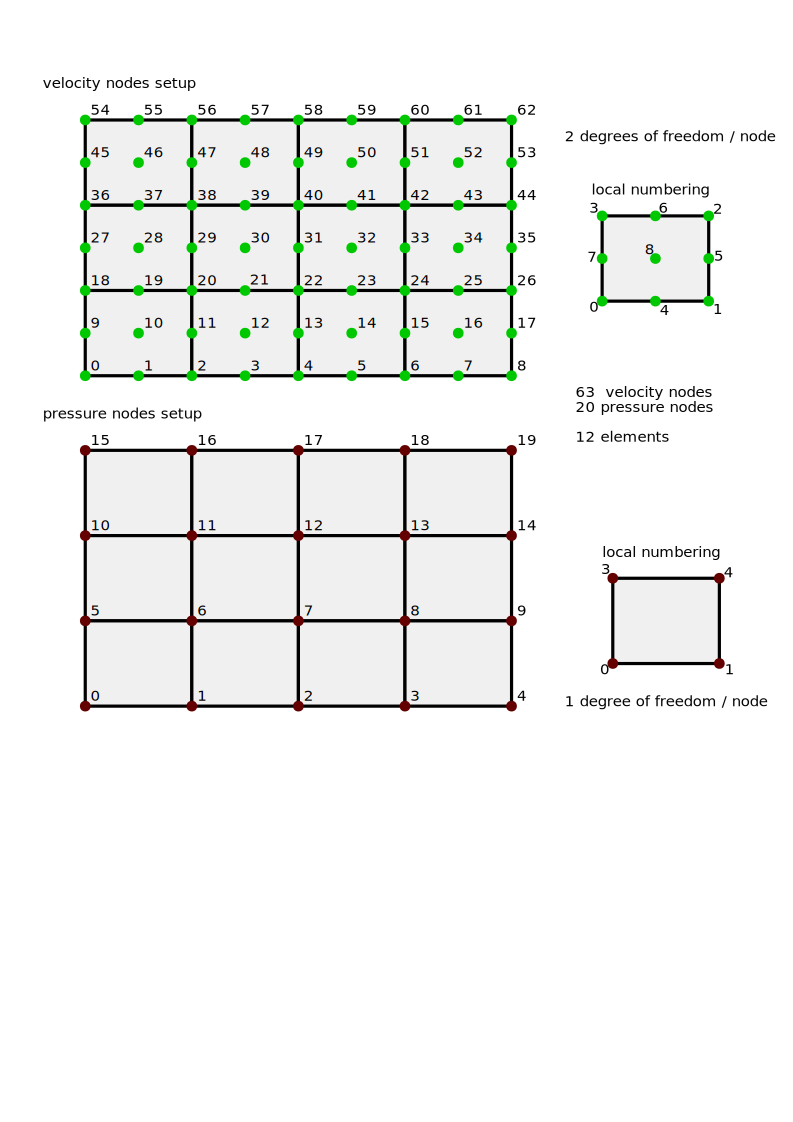
\includegraphics[width=10cm]{python_codes/fieldstone_18/images/q2q1setup}
\end{center}

%-----------------------------------------
\subsection*{Donea \& Huerta benchmark ({\tt bench=1})}
The details of the numerical setup are presented in Section \ref{MMM-mms1}.

\begin{center}
\includegraphics[width=7cm]{python_codes/fieldstone_18/results/mms/vel}
\includegraphics[width=7cm]{python_codes/fieldstone_18/results/mms/pressure}\\
{\captionfont Velocity and pressure fields for $32\times 32$ elements grid}
\end{center}

\begin{center}
\includegraphics[width=12cm]{python_codes/fieldstone_18/results/mms/errors}\\
{\captionfont Velocity and pressure error convergence for both nullspace removal 
techniques. The zero average pressure approach yields smaller errors.}
\end{center}

\newpage
%-----------------------------------------
\subsection*{Burman \& Hansbo manufactured solution ({\tt bench=4})}

The details of the numerical setup are presented in Section \ref{MMM-ss:mms_buha06}.
The velocity and pressure fields are given in the unit square by
\begin{eqnarray}
u(x,y) &=& 20xy^3 \nn\\
v(x,y) &=& 5x^4-5y^4 \nn\\
p(x,y) &=& 60x^2y -20y^3 -5
\end{eqnarray}
The analytical velocity is prescribed on all sides of the domain.

\begin{center}
\includegraphics[width=7cm]{python_codes/fieldstone_18/results/buha06/vel}
\includegraphics[width=7cm]{python_codes/fieldstone_18/results/buha06/p}\\
{\captionfont Velocity and pressure fields for $64\times 64$ elements grid}
\end{center}

\begin{center}
\includegraphics[width=8cm]{python_codes/fieldstone_18/results/buha06/errorsV}
\includegraphics[width=8cm]{python_codes/fieldstone_18/results/buha06/errorsP}\\
{\captionfont Velocity and pressure error convergence. Zero average.}
\end{center}

The conclusion is clear (and expected): there is no good reason 
to run such higher numbers of quadrature points.


\newpage
%----------------------------------------------------
\subsection*{Stokes sphere benchmark ({\tt bench=2})}

The setup is described in Section~\ref{MMM-ss:stokes_sphere2D}.
The domain is the unit square.
A sphere of radius 0.123456789 is placed in the middle of the domain. 
Its density is 1.01 while the density of the surrounding fluid is 1,
while its viscosity is 1000 times larger than the viscosity of the fluid.
Gravity is pointing downward with $|g|=1$.
There is no analytical solution to this problem.
Either no-slip or free-slip boundary conditions are prescribed on all 
sides.

\subsubsection*{Free-slip boundary conditions (FS)}

\begin{center}
\includegraphics[width=5.7cm]{python_codes/fieldstone_18/results/sphere/FS/vel}
\includegraphics[width=5.7cm]{python_codes/fieldstone_18/results/sphere/FS/press}
\includegraphics[width=5.7cm]{python_codes/fieldstone_18/results/sphere/FS/divv}\\
{\captionfont Velocity, pressure and velocity divergence fields for $48\times 48$ 
elements grid and $3^2$ quadrature points per element.}
\end{center}






\subsubsection*{No-slip boundary conditions (NS)}

\begin{center}
\includegraphics[width=5.7cm]{python_codes/fieldstone_18/results/sphere/NS/vel}
\includegraphics[width=5.7cm]{python_codes/fieldstone_18/results/sphere/NS/press}
\includegraphics[width=5.7cm]{python_codes/fieldstone_18/results/sphere/NS/divv}\\
{\captionfont Velocity, pressure and velocity divergence fields for $48\times 48$ 
elements grid and $3^2$ quadrature points per element.}
\end{center}




\newpage
%-----------------------------------------
\subsection*{Sinking block benchmark ({\tt bench=3})}

The setup is described in Section~\ref{MMM-ss:sinking_block} of part 1.
The domain is the unit square.
A block of density $\rho=1.01$ is placed in a fluid of density $\rho=1$.
The gravity is vertical and pointing downward with $|\vec{g}|=1$.
The function for $b_y$ is then:
\begin{lstlisting}
def by(x,y):
    [...]
    if abs(x-.5)<0.0625 and abs(y-0.5)<0.0625:
       val=-1.01
   else:
      val=-1.
\end{lstlisting}
The block is 1000 times more viscous than the fluid:
\begin{lstlisting}
def eta(x,y):
    [...]
    if bench==3:
       if abs(x-.5)<0.0625 and abs(y-0.5)<0.0625:
          val=1000
       else:
          val=1
\end{lstlisting}





\subsubsection*{Free slip boundary conditions (FS)}

\begin{center}
\includegraphics[width=7cm]{python_codes/fieldstone_18/results/block/FS/vel}
\includegraphics[width=7cm]{python_codes/fieldstone_18/results/block/FS/press}\\
{\captionfont Velocity and pressure fields for $48\times 48$ elements grid and $3^2$
quadrature points per element.}
\end{center}


\begin{center}
\includegraphics[width=5.7cm]{python_codes/fieldstone_18/results/block/vrms}
\includegraphics[width=5.7cm]{python_codes/fieldstone_18/results/block/max_vel}\\
\includegraphics[width=5.7cm]{python_codes/fieldstone_18/results/block/min_u}
\includegraphics[width=5.7cm]{python_codes/fieldstone_18/results/block/max_u}\\
\includegraphics[width=5.7cm]{python_codes/fieldstone_18/results/block/min_v}
\includegraphics[width=5.7cm]{python_codes/fieldstone_18/results/block/max_v}\\
\includegraphics[width=5.7cm]{python_codes/fieldstone_18/results/block/min_p}
\includegraphics[width=5.7cm]{python_codes/fieldstone_18/results/block/max_p}\\
\includegraphics[width=5.7cm]{python_codes/fieldstone_18/results/block/profile_u_FS}
\includegraphics[width=5.7cm]{python_codes/fieldstone_18/results/block/profile_v_FS}
\includegraphics[width=5.7cm]{python_codes/fieldstone_18/results/block/profile_p_FS}
\end{center}

%.....................................................
\subsubsection*{No slip boundary conditions (NS)}

\begin{center}
\includegraphics[width=5.7cm]{python_codes/fieldstone_18/results/block/NS/u}
\includegraphics[width=5.7cm]{python_codes/fieldstone_18/results/block/NS/v}
\includegraphics[width=5.7cm]{python_codes/fieldstone_18/results/block/NS/p}\\
{\captionfont Velocity and pressure fields for $32\times 32$ elements grid and $3^2$
quadrature points per element.}
\end{center}

Velocity and pressure are also measured on a vertical line going through
the middle of the domain/block (the lithostatic pressure is 
subtracted from the computed full pressure so that what is plotted is the 
dynamic pressure):
\begin{center}
\includegraphics[width=5.7cm]{python_codes/fieldstone_18/results/block/profile_u_NS}
\includegraphics[width=5.7cm]{python_codes/fieldstone_18/results/block/profile_v_NS}
\includegraphics[width=5.7cm]{python_codes/fieldstone_18/results/block/profile_p_NS}
\end{center}
As expected, the $x$ component of the velocity is zero because of symmetry.


\newpage
%----------------------------------------------------
\subsection*{Inclusion in pure shear ({\tt bench=5})}

(this setup was created for Philippe Yamato of Rennes University)

The inclusion is placed at the origin and has a radius 0.1, while the domain is the 
unit square. Viscosity inside the inclusion is 1 while the matrix viscosity is 1000.
Free slip is prescribed on the left and bottom boundary while 
$u=-1$ is prescribed on the right boundary and $v=+1$ on the top.

\begin{center}
\includegraphics[width=5.7cm]{python_codes/fieldstone_18/results/inclusion/eta}
\includegraphics[width=5.7cm]{python_codes/fieldstone_18/results/inclusion/vel}
\includegraphics[width=5.7cm]{python_codes/fieldstone_18/results/inclusion/press}\\
{\captionfont Resolution $256\times 256$.}
\end{center}

Note that viscosity is prescribed on quadrature levels, which in this case 
is likely to generate large errors/jumps around the inclusion surface.

\begin{verbatim}
For 256x256 mesh on my laptop:
setup: grid points: 0.128 s
setup: connectivity: 0.242 s
setup: boundary conditions: 0.151 s
build FE matrix: 284.284 s
assemble blocks: 0.003 s
solve time: 804.607 s
\end{verbatim}





\newpage
%%%%%%%%%%%%%%%%%%%%%%%%%%%%%%%%%%%%%%%%%%%%%%%%%%%%%%%%%%%%%%%%%%%%%%%%%%%%%%%
\section{{\tt fieldstone}: solvi benchmark}
\includegraphics[height=1.25cm]{images/pictograms/benchmark}
\includegraphics[height=1.25cm]{images/pictograms/FEM}

%%%%%%%%%%%%%%%%%%%%%%%%%%%%%%%%%%%%%%%%%%%%%%%%%%%%%%%%%%%%%%%%%%%%%%%%%%%%%%%%%%%%%%%%%%%%%%%%%%%

%\lstinputlisting[language=bash,basicstyle=\small]{python_codes/fieldstone_18/keywords.key}

\begin{center}
\inpython
{\small Code: \url{https://github.com/cedrict/fieldstone/tree/master/python_codes/fieldstone_18}}
\end{center}

\par\noindent\rule{\textwidth}{0.4pt}

Last revision: Feb. 7th, 2025.

\par\noindent\rule{\textwidth}{0.4pt}

%%%%%%%%%%%%%%%%%%%%%%%%%%%%%%%%%%%%%%%%%%%%%%%%%%%%%%%%%%%%%%%%%%%%%%%%%%%%%%%%%%%%%%%%%%%%%%%%%%%

The code relies on \QtwoQone elements.
Each element has $m_V=9$ vertices so in total $ndof_V\times m_V=18$ velocity dofs and 
$ndof_P*m_P=4$ pressure dofs. The total number of 
velocity dofs is therefore $NfemV=NV \times ndofV$ while the total number of
pressure dofs is $NfemP=NP\times ndofP$. The total number of dofs is then $Nfem=NfemV+NfemP$.

As a consequence, matrix $\K$ has size $NfemV,NfemV$ and matrix $\G$ has size $NfemV,NfemP$.
Vector $f$ is of size $NfemV$ and vector $h$ is of size $NfemP$.  

When needed the pressure nullspace is removed 
by imposing (Lagrange multiplier) that $\int_\Omega p \; dV=0$.

The following figure shows the layout of velocity and pressure nodes
for a $4\times 3$ element mesh:
\begin{center}
\includegraphics[width=10cm]{python_codes/fieldstone_18/images/q2q1setup}
\end{center}

%-----------------------------------------
\subsection*{Donea \& Huerta benchmark ({\tt bench=1})}
The details of the numerical setup are presented in Section \ref{MMM-mms1}.

\begin{center}
\includegraphics[width=7cm]{python_codes/fieldstone_18/results/mms/vel}
\includegraphics[width=7cm]{python_codes/fieldstone_18/results/mms/pressure}\\
{\captionfont Velocity and pressure fields for $32\times 32$ elements grid}
\end{center}

\begin{center}
\includegraphics[width=12cm]{python_codes/fieldstone_18/results/mms/errors}\\
{\captionfont Velocity and pressure error convergence for both nullspace removal 
techniques. The zero average pressure approach yields smaller errors.}
\end{center}

\newpage
%-----------------------------------------
\subsection*{Burman \& Hansbo manufactured solution ({\tt bench=4})}

The details of the numerical setup are presented in Section \ref{MMM-ss:mms_buha06}.
The velocity and pressure fields are given in the unit square by
\begin{eqnarray}
u(x,y) &=& 20xy^3 \nn\\
v(x,y) &=& 5x^4-5y^4 \nn\\
p(x,y) &=& 60x^2y -20y^3 -5
\end{eqnarray}
The analytical velocity is prescribed on all sides of the domain.

\begin{center}
\includegraphics[width=7cm]{python_codes/fieldstone_18/results/buha06/vel}
\includegraphics[width=7cm]{python_codes/fieldstone_18/results/buha06/p}\\
{\captionfont Velocity and pressure fields for $64\times 64$ elements grid}
\end{center}

\begin{center}
\includegraphics[width=8cm]{python_codes/fieldstone_18/results/buha06/errorsV}
\includegraphics[width=8cm]{python_codes/fieldstone_18/results/buha06/errorsP}\\
{\captionfont Velocity and pressure error convergence. Zero average.}
\end{center}

The conclusion is clear (and expected): there is no good reason 
to run such higher numbers of quadrature points.


\newpage
%----------------------------------------------------
\subsection*{Stokes sphere benchmark ({\tt bench=2})}

The setup is described in Section~\ref{MMM-ss:stokes_sphere2D}.
The domain is the unit square.
A sphere of radius 0.123456789 is placed in the middle of the domain. 
Its density is 1.01 while the density of the surrounding fluid is 1,
while its viscosity is 1000 times larger than the viscosity of the fluid.
Gravity is pointing downward with $|g|=1$.
There is no analytical solution to this problem.
Either no-slip or free-slip boundary conditions are prescribed on all 
sides.

\subsubsection*{Free-slip boundary conditions (FS)}

\begin{center}
\includegraphics[width=5.7cm]{python_codes/fieldstone_18/results/sphere/FS/vel}
\includegraphics[width=5.7cm]{python_codes/fieldstone_18/results/sphere/FS/press}
\includegraphics[width=5.7cm]{python_codes/fieldstone_18/results/sphere/FS/divv}\\
{\captionfont Velocity, pressure and velocity divergence fields for $48\times 48$ 
elements grid and $3^2$ quadrature points per element.}
\end{center}






\subsubsection*{No-slip boundary conditions (NS)}

\begin{center}
\includegraphics[width=5.7cm]{python_codes/fieldstone_18/results/sphere/NS/vel}
\includegraphics[width=5.7cm]{python_codes/fieldstone_18/results/sphere/NS/press}
\includegraphics[width=5.7cm]{python_codes/fieldstone_18/results/sphere/NS/divv}\\
{\captionfont Velocity, pressure and velocity divergence fields for $48\times 48$ 
elements grid and $3^2$ quadrature points per element.}
\end{center}




\newpage
%-----------------------------------------
\subsection*{Sinking block benchmark ({\tt bench=3})}

The setup is described in Section~\ref{MMM-ss:sinking_block} of part 1.
The domain is the unit square.
A block of density $\rho=1.01$ is placed in a fluid of density $\rho=1$.
The gravity is vertical and pointing downward with $|\vec{g}|=1$.
The function for $b_y$ is then:
\begin{lstlisting}
def by(x,y):
    [...]
    if abs(x-.5)<0.0625 and abs(y-0.5)<0.0625:
       val=-1.01
   else:
      val=-1.
\end{lstlisting}
The block is 1000 times more viscous than the fluid:
\begin{lstlisting}
def eta(x,y):
    [...]
    if bench==3:
       if abs(x-.5)<0.0625 and abs(y-0.5)<0.0625:
          val=1000
       else:
          val=1
\end{lstlisting}





\subsubsection*{Free slip boundary conditions (FS)}

\begin{center}
\includegraphics[width=7cm]{python_codes/fieldstone_18/results/block/FS/vel}
\includegraphics[width=7cm]{python_codes/fieldstone_18/results/block/FS/press}\\
{\captionfont Velocity and pressure fields for $48\times 48$ elements grid and $3^2$
quadrature points per element.}
\end{center}


\begin{center}
\includegraphics[width=5.7cm]{python_codes/fieldstone_18/results/block/vrms}
\includegraphics[width=5.7cm]{python_codes/fieldstone_18/results/block/max_vel}\\
\includegraphics[width=5.7cm]{python_codes/fieldstone_18/results/block/min_u}
\includegraphics[width=5.7cm]{python_codes/fieldstone_18/results/block/max_u}\\
\includegraphics[width=5.7cm]{python_codes/fieldstone_18/results/block/min_v}
\includegraphics[width=5.7cm]{python_codes/fieldstone_18/results/block/max_v}\\
\includegraphics[width=5.7cm]{python_codes/fieldstone_18/results/block/min_p}
\includegraphics[width=5.7cm]{python_codes/fieldstone_18/results/block/max_p}\\
\includegraphics[width=5.7cm]{python_codes/fieldstone_18/results/block/profile_u_FS}
\includegraphics[width=5.7cm]{python_codes/fieldstone_18/results/block/profile_v_FS}
\includegraphics[width=5.7cm]{python_codes/fieldstone_18/results/block/profile_p_FS}
\end{center}

%.....................................................
\subsubsection*{No slip boundary conditions (NS)}

\begin{center}
\includegraphics[width=5.7cm]{python_codes/fieldstone_18/results/block/NS/u}
\includegraphics[width=5.7cm]{python_codes/fieldstone_18/results/block/NS/v}
\includegraphics[width=5.7cm]{python_codes/fieldstone_18/results/block/NS/p}\\
{\captionfont Velocity and pressure fields for $32\times 32$ elements grid and $3^2$
quadrature points per element.}
\end{center}

Velocity and pressure are also measured on a vertical line going through
the middle of the domain/block (the lithostatic pressure is 
subtracted from the computed full pressure so that what is plotted is the 
dynamic pressure):
\begin{center}
\includegraphics[width=5.7cm]{python_codes/fieldstone_18/results/block/profile_u_NS}
\includegraphics[width=5.7cm]{python_codes/fieldstone_18/results/block/profile_v_NS}
\includegraphics[width=5.7cm]{python_codes/fieldstone_18/results/block/profile_p_NS}
\end{center}
As expected, the $x$ component of the velocity is zero because of symmetry.


\newpage
%----------------------------------------------------
\subsection*{Inclusion in pure shear ({\tt bench=5})}

(this setup was created for Philippe Yamato of Rennes University)

The inclusion is placed at the origin and has a radius 0.1, while the domain is the 
unit square. Viscosity inside the inclusion is 1 while the matrix viscosity is 1000.
Free slip is prescribed on the left and bottom boundary while 
$u=-1$ is prescribed on the right boundary and $v=+1$ on the top.

\begin{center}
\includegraphics[width=5.7cm]{python_codes/fieldstone_18/results/inclusion/eta}
\includegraphics[width=5.7cm]{python_codes/fieldstone_18/results/inclusion/vel}
\includegraphics[width=5.7cm]{python_codes/fieldstone_18/results/inclusion/press}\\
{\captionfont Resolution $256\times 256$.}
\end{center}

Note that viscosity is prescribed on quadrature levels, which in this case 
is likely to generate large errors/jumps around the inclusion surface.

\begin{verbatim}
For 256x256 mesh on my laptop:
setup: grid points: 0.128 s
setup: connectivity: 0.242 s
setup: boundary conditions: 0.151 s
build FE matrix: 284.284 s
assemble blocks: 0.003 s
solve time: 804.607 s
\end{verbatim}





\newpage
%%%%%%%%%%%%%%%%%%%%%%%%%%%%%%%%%%%%%%%%%%%%%%%%%%%%%%%%%%%%%%%%%%%%%%%%%%%%%%%
\section{{\tt fieldstone}: the indentor benchmark}

The punch benchmark is one of the few boundary value problems involving plastic solids for which there exists an exact solution. 
Such solutions are usually either for highly simplified geometries (spherical or axial symmetry, for instance) or simplified material models (such as rigid plastic solids) \cite{kacha04}.

In this experiment, a rigid punch indents a rigid plastic half space; the slip line field theory gives 
exact solutions as shown in Fig. \ref{fig_punch}a. 
The plane strain formulation of the equations and the detailed solution to the problem were derived in the Appendix of \cite{thfb08} and are also presented in \cite{gepd98}.

The two dimensional punch problem has been extensively studied numerically for the past 40 years 
\cite{zihl75,zihp95,chpe01,chan99,huhy99,yuti06,bufs08,raab07} and has been used to draw a parallel with the tectonics of eastern China in the context of the 
India-Eurasia collision \cite{tamo76,mota77}.
It is also worth noting that it has been carried out in one form or another in series of 
analogue modelling articles 
concerning the same region, with a rigid indenter colliding with a rheologically stratified lithosphere \cite{peta88,daco88,jodc90}.

 
Numerically, the one-time step punch experiment is performed on a two-dimensional
domain of purely plastic von Mises material. 
Given that the von Mises rheology yield criterion does not depend on pressure, the density of the material and/or the gravity vector is set to zero. Sides are set to free slip boundary conditions, the bottom to no slip, while a vertical velocity $(0,-v_p)$ is prescribed at the top boundary for nodes whose $x$ coordinate is within $[L_x/2-\delta/2,L_x/2+\delta/2]$. 

The following parameters are used: $L_x=1$, $L_y=0.5$, $\mu_{min}=10^{-3}$, 
$\mu_{max}=10^3$, $v_p=1$, $\delta=0.123456789$ 
and the yield value of the material is set to $k=1$. 

The analytical solution predicts that the angle of the shear bands stemming from the sides of the punch 
is $\pi/4$, that the pressure right under the punch is $1+\pi$, 
and that the velocity of the rigid blocks on each side of the punch is $v_p/\sqrt{2}$ 
(this is simply explained by invoking conservation of mass).

\includegraphics[width=16cm]{python_codes/fieldstone_indentor/solution.pdf}

ToDo: smooth punch

\fbox{
\parbox{10cm}{{\bf features}
\begin{itemize}
\item $Q_1\times P_0$ element \index{$Q_1 \times P_0$}
\item incompressible flow \index{incompressible flow}
\item penalty formulation \index{penalty formulation}
\item Dirichlet boundary conditions (no-slip)
\item isothermal \index{isothermal}
\item non-isoviscous \index{non-isoviscous}
\item nonlinear rheology \index{nonlinear rheology}
\end{itemize}
}}



\newpage
%%%%%%%%%%%%%%%%%%%%%%%%%%%%%%%%%%%%%%%%%%%%%%%%%%%%%%%%%%%%%%%%%%%%%%%%%%%%%%%
\section{{\tt fieldstone}: the annulus benchmark}
\includegraphics[height=1.25cm]{images/pictograms/benchmark}
\includegraphics[height=1.25cm]{images/pictograms/FEM}

%%%%%%%%%%%%%%%%%%%%%%%%%%%%%%%%%%%%%%%%%%%%%%%%%%%%%%%%%%%%%%%%%%%%%%%%%%%%%%%%%%%%%%%%%%%%%%%%%%%

%\lstinputlisting[language=bash,basicstyle=\small]{python_codes/fieldstone_18/keywords.key}

\begin{center}
\inpython
{\small Code: \url{https://github.com/cedrict/fieldstone/tree/master/python_codes/fieldstone_18}}
\end{center}

\par\noindent\rule{\textwidth}{0.4pt}

Last revision: Feb. 7th, 2025.

\par\noindent\rule{\textwidth}{0.4pt}

%%%%%%%%%%%%%%%%%%%%%%%%%%%%%%%%%%%%%%%%%%%%%%%%%%%%%%%%%%%%%%%%%%%%%%%%%%%%%%%%%%%%%%%%%%%%%%%%%%%

The code relies on \QtwoQone elements.
Each element has $m_V=9$ vertices so in total $ndof_V\times m_V=18$ velocity dofs and 
$ndof_P*m_P=4$ pressure dofs. The total number of 
velocity dofs is therefore $NfemV=NV \times ndofV$ while the total number of
pressure dofs is $NfemP=NP\times ndofP$. The total number of dofs is then $Nfem=NfemV+NfemP$.

As a consequence, matrix $\K$ has size $NfemV,NfemV$ and matrix $\G$ has size $NfemV,NfemP$.
Vector $f$ is of size $NfemV$ and vector $h$ is of size $NfemP$.  

When needed the pressure nullspace is removed 
by imposing (Lagrange multiplier) that $\int_\Omega p \; dV=0$.

The following figure shows the layout of velocity and pressure nodes
for a $4\times 3$ element mesh:
\begin{center}
\includegraphics[width=10cm]{python_codes/fieldstone_18/images/q2q1setup}
\end{center}

%-----------------------------------------
\subsection*{Donea \& Huerta benchmark ({\tt bench=1})}
The details of the numerical setup are presented in Section \ref{MMM-mms1}.

\begin{center}
\includegraphics[width=7cm]{python_codes/fieldstone_18/results/mms/vel}
\includegraphics[width=7cm]{python_codes/fieldstone_18/results/mms/pressure}\\
{\captionfont Velocity and pressure fields for $32\times 32$ elements grid}
\end{center}

\begin{center}
\includegraphics[width=12cm]{python_codes/fieldstone_18/results/mms/errors}\\
{\captionfont Velocity and pressure error convergence for both nullspace removal 
techniques. The zero average pressure approach yields smaller errors.}
\end{center}

\newpage
%-----------------------------------------
\subsection*{Burman \& Hansbo manufactured solution ({\tt bench=4})}

The details of the numerical setup are presented in Section \ref{MMM-ss:mms_buha06}.
The velocity and pressure fields are given in the unit square by
\begin{eqnarray}
u(x,y) &=& 20xy^3 \nn\\
v(x,y) &=& 5x^4-5y^4 \nn\\
p(x,y) &=& 60x^2y -20y^3 -5
\end{eqnarray}
The analytical velocity is prescribed on all sides of the domain.

\begin{center}
\includegraphics[width=7cm]{python_codes/fieldstone_18/results/buha06/vel}
\includegraphics[width=7cm]{python_codes/fieldstone_18/results/buha06/p}\\
{\captionfont Velocity and pressure fields for $64\times 64$ elements grid}
\end{center}

\begin{center}
\includegraphics[width=8cm]{python_codes/fieldstone_18/results/buha06/errorsV}
\includegraphics[width=8cm]{python_codes/fieldstone_18/results/buha06/errorsP}\\
{\captionfont Velocity and pressure error convergence. Zero average.}
\end{center}

The conclusion is clear (and expected): there is no good reason 
to run such higher numbers of quadrature points.


\newpage
%----------------------------------------------------
\subsection*{Stokes sphere benchmark ({\tt bench=2})}

The setup is described in Section~\ref{MMM-ss:stokes_sphere2D}.
The domain is the unit square.
A sphere of radius 0.123456789 is placed in the middle of the domain. 
Its density is 1.01 while the density of the surrounding fluid is 1,
while its viscosity is 1000 times larger than the viscosity of the fluid.
Gravity is pointing downward with $|g|=1$.
There is no analytical solution to this problem.
Either no-slip or free-slip boundary conditions are prescribed on all 
sides.

\subsubsection*{Free-slip boundary conditions (FS)}

\begin{center}
\includegraphics[width=5.7cm]{python_codes/fieldstone_18/results/sphere/FS/vel}
\includegraphics[width=5.7cm]{python_codes/fieldstone_18/results/sphere/FS/press}
\includegraphics[width=5.7cm]{python_codes/fieldstone_18/results/sphere/FS/divv}\\
{\captionfont Velocity, pressure and velocity divergence fields for $48\times 48$ 
elements grid and $3^2$ quadrature points per element.}
\end{center}






\subsubsection*{No-slip boundary conditions (NS)}

\begin{center}
\includegraphics[width=5.7cm]{python_codes/fieldstone_18/results/sphere/NS/vel}
\includegraphics[width=5.7cm]{python_codes/fieldstone_18/results/sphere/NS/press}
\includegraphics[width=5.7cm]{python_codes/fieldstone_18/results/sphere/NS/divv}\\
{\captionfont Velocity, pressure and velocity divergence fields for $48\times 48$ 
elements grid and $3^2$ quadrature points per element.}
\end{center}




\newpage
%-----------------------------------------
\subsection*{Sinking block benchmark ({\tt bench=3})}

The setup is described in Section~\ref{MMM-ss:sinking_block} of part 1.
The domain is the unit square.
A block of density $\rho=1.01$ is placed in a fluid of density $\rho=1$.
The gravity is vertical and pointing downward with $|\vec{g}|=1$.
The function for $b_y$ is then:
\begin{lstlisting}
def by(x,y):
    [...]
    if abs(x-.5)<0.0625 and abs(y-0.5)<0.0625:
       val=-1.01
   else:
      val=-1.
\end{lstlisting}
The block is 1000 times more viscous than the fluid:
\begin{lstlisting}
def eta(x,y):
    [...]
    if bench==3:
       if abs(x-.5)<0.0625 and abs(y-0.5)<0.0625:
          val=1000
       else:
          val=1
\end{lstlisting}





\subsubsection*{Free slip boundary conditions (FS)}

\begin{center}
\includegraphics[width=7cm]{python_codes/fieldstone_18/results/block/FS/vel}
\includegraphics[width=7cm]{python_codes/fieldstone_18/results/block/FS/press}\\
{\captionfont Velocity and pressure fields for $48\times 48$ elements grid and $3^2$
quadrature points per element.}
\end{center}


\begin{center}
\includegraphics[width=5.7cm]{python_codes/fieldstone_18/results/block/vrms}
\includegraphics[width=5.7cm]{python_codes/fieldstone_18/results/block/max_vel}\\
\includegraphics[width=5.7cm]{python_codes/fieldstone_18/results/block/min_u}
\includegraphics[width=5.7cm]{python_codes/fieldstone_18/results/block/max_u}\\
\includegraphics[width=5.7cm]{python_codes/fieldstone_18/results/block/min_v}
\includegraphics[width=5.7cm]{python_codes/fieldstone_18/results/block/max_v}\\
\includegraphics[width=5.7cm]{python_codes/fieldstone_18/results/block/min_p}
\includegraphics[width=5.7cm]{python_codes/fieldstone_18/results/block/max_p}\\
\includegraphics[width=5.7cm]{python_codes/fieldstone_18/results/block/profile_u_FS}
\includegraphics[width=5.7cm]{python_codes/fieldstone_18/results/block/profile_v_FS}
\includegraphics[width=5.7cm]{python_codes/fieldstone_18/results/block/profile_p_FS}
\end{center}

%.....................................................
\subsubsection*{No slip boundary conditions (NS)}

\begin{center}
\includegraphics[width=5.7cm]{python_codes/fieldstone_18/results/block/NS/u}
\includegraphics[width=5.7cm]{python_codes/fieldstone_18/results/block/NS/v}
\includegraphics[width=5.7cm]{python_codes/fieldstone_18/results/block/NS/p}\\
{\captionfont Velocity and pressure fields for $32\times 32$ elements grid and $3^2$
quadrature points per element.}
\end{center}

Velocity and pressure are also measured on a vertical line going through
the middle of the domain/block (the lithostatic pressure is 
subtracted from the computed full pressure so that what is plotted is the 
dynamic pressure):
\begin{center}
\includegraphics[width=5.7cm]{python_codes/fieldstone_18/results/block/profile_u_NS}
\includegraphics[width=5.7cm]{python_codes/fieldstone_18/results/block/profile_v_NS}
\includegraphics[width=5.7cm]{python_codes/fieldstone_18/results/block/profile_p_NS}
\end{center}
As expected, the $x$ component of the velocity is zero because of symmetry.


\newpage
%----------------------------------------------------
\subsection*{Inclusion in pure shear ({\tt bench=5})}

(this setup was created for Philippe Yamato of Rennes University)

The inclusion is placed at the origin and has a radius 0.1, while the domain is the 
unit square. Viscosity inside the inclusion is 1 while the matrix viscosity is 1000.
Free slip is prescribed on the left and bottom boundary while 
$u=-1$ is prescribed on the right boundary and $v=+1$ on the top.

\begin{center}
\includegraphics[width=5.7cm]{python_codes/fieldstone_18/results/inclusion/eta}
\includegraphics[width=5.7cm]{python_codes/fieldstone_18/results/inclusion/vel}
\includegraphics[width=5.7cm]{python_codes/fieldstone_18/results/inclusion/press}\\
{\captionfont Resolution $256\times 256$.}
\end{center}

Note that viscosity is prescribed on quadrature levels, which in this case 
is likely to generate large errors/jumps around the inclusion surface.

\begin{verbatim}
For 256x256 mesh on my laptop:
setup: grid points: 0.128 s
setup: connectivity: 0.242 s
setup: boundary conditions: 0.151 s
build FE matrix: 284.284 s
assemble blocks: 0.003 s
solve time: 804.607 s
\end{verbatim}






\newpage
%%%%%%%%%%%%%%%%%%%%%%%%%%%%%%%%%%%%%%%%%%%%%%%%%%%%%%%%%%%%%%%%%%%%%%%%%%%%%%%
\section{{\tt fieldstone}: stokes sphere (3D) - penalty\label{f5}}

\fbox{
\parbox{10cm}{{\bf features}
\begin{itemize}
\item $Q_1\times P_0$ element
\item incompressible flow
\item penalty formulation
\item Dirichlet boundary conditions (free-slip)
\item direct solver
\item isothermal
\item non-isoviscous
\item 3D
\item elemental b.c. 
\item buoyancy driven
\end{itemize}
}}


\begin{center}
\includegraphics[width=5cm]{python_codes/fieldstone_stokes_sphere_3D/grid}
\includegraphics[width=5cm]{python_codes/fieldstone_stokes_sphere_3D/vel}
\includegraphics[width=5cm]{python_codes/fieldstone_stokes_sphere_3D/press}\\
\includegraphics[width=5cm]{python_codes/fieldstone_stokes_sphere_3D/press2}
\includegraphics[width=5cm]{python_codes/fieldstone_stokes_sphere_3D/visc}
\includegraphics[width=5cm]{python_codes/fieldstone_stokes_sphere_3D/dens}\\
{\small resolution is 24x24x24}
\end{center}



\newpage
%%%%%%%%%%%%%%%%%%%%%%%%%%%%%%%%%%%%%%%%%%%%%%%%%%%%%%%%%%%%%%%%%%%%%%%%%%%%%%%
\section{{\tt fieldstone}: stokes sphere (3D) - mixed formulation\label{f5}}
\includegraphics[height=1.25cm]{images/pictograms/benchmark}
\includegraphics[height=1.25cm]{images/pictograms/FEM}

%%%%%%%%%%%%%%%%%%%%%%%%%%%%%%%%%%%%%%%%%%%%%%%%%%%%%%%%%%%%%%%%%%%%%%%%%%%%%%%%%%%%%%%%%%%%%%%%%%%

%\lstinputlisting[language=bash,basicstyle=\small]{python_codes/fieldstone_18/keywords.key}

\begin{center}
\inpython
{\small Code: \url{https://github.com/cedrict/fieldstone/tree/master/python_codes/fieldstone_18}}
\end{center}

\par\noindent\rule{\textwidth}{0.4pt}

Last revision: Feb. 7th, 2025.

\par\noindent\rule{\textwidth}{0.4pt}

%%%%%%%%%%%%%%%%%%%%%%%%%%%%%%%%%%%%%%%%%%%%%%%%%%%%%%%%%%%%%%%%%%%%%%%%%%%%%%%%%%%%%%%%%%%%%%%%%%%

The code relies on \QtwoQone elements.
Each element has $m_V=9$ vertices so in total $ndof_V\times m_V=18$ velocity dofs and 
$ndof_P*m_P=4$ pressure dofs. The total number of 
velocity dofs is therefore $NfemV=NV \times ndofV$ while the total number of
pressure dofs is $NfemP=NP\times ndofP$. The total number of dofs is then $Nfem=NfemV+NfemP$.

As a consequence, matrix $\K$ has size $NfemV,NfemV$ and matrix $\G$ has size $NfemV,NfemP$.
Vector $f$ is of size $NfemV$ and vector $h$ is of size $NfemP$.  

When needed the pressure nullspace is removed 
by imposing (Lagrange multiplier) that $\int_\Omega p \; dV=0$.

The following figure shows the layout of velocity and pressure nodes
for a $4\times 3$ element mesh:
\begin{center}
\includegraphics[width=10cm]{python_codes/fieldstone_18/images/q2q1setup}
\end{center}

%-----------------------------------------
\subsection*{Donea \& Huerta benchmark ({\tt bench=1})}
The details of the numerical setup are presented in Section \ref{MMM-mms1}.

\begin{center}
\includegraphics[width=7cm]{python_codes/fieldstone_18/results/mms/vel}
\includegraphics[width=7cm]{python_codes/fieldstone_18/results/mms/pressure}\\
{\captionfont Velocity and pressure fields for $32\times 32$ elements grid}
\end{center}

\begin{center}
\includegraphics[width=12cm]{python_codes/fieldstone_18/results/mms/errors}\\
{\captionfont Velocity and pressure error convergence for both nullspace removal 
techniques. The zero average pressure approach yields smaller errors.}
\end{center}

\newpage
%-----------------------------------------
\subsection*{Burman \& Hansbo manufactured solution ({\tt bench=4})}

The details of the numerical setup are presented in Section \ref{MMM-ss:mms_buha06}.
The velocity and pressure fields are given in the unit square by
\begin{eqnarray}
u(x,y) &=& 20xy^3 \nn\\
v(x,y) &=& 5x^4-5y^4 \nn\\
p(x,y) &=& 60x^2y -20y^3 -5
\end{eqnarray}
The analytical velocity is prescribed on all sides of the domain.

\begin{center}
\includegraphics[width=7cm]{python_codes/fieldstone_18/results/buha06/vel}
\includegraphics[width=7cm]{python_codes/fieldstone_18/results/buha06/p}\\
{\captionfont Velocity and pressure fields for $64\times 64$ elements grid}
\end{center}

\begin{center}
\includegraphics[width=8cm]{python_codes/fieldstone_18/results/buha06/errorsV}
\includegraphics[width=8cm]{python_codes/fieldstone_18/results/buha06/errorsP}\\
{\captionfont Velocity and pressure error convergence. Zero average.}
\end{center}

The conclusion is clear (and expected): there is no good reason 
to run such higher numbers of quadrature points.


\newpage
%----------------------------------------------------
\subsection*{Stokes sphere benchmark ({\tt bench=2})}

The setup is described in Section~\ref{MMM-ss:stokes_sphere2D}.
The domain is the unit square.
A sphere of radius 0.123456789 is placed in the middle of the domain. 
Its density is 1.01 while the density of the surrounding fluid is 1,
while its viscosity is 1000 times larger than the viscosity of the fluid.
Gravity is pointing downward with $|g|=1$.
There is no analytical solution to this problem.
Either no-slip or free-slip boundary conditions are prescribed on all 
sides.

\subsubsection*{Free-slip boundary conditions (FS)}

\begin{center}
\includegraphics[width=5.7cm]{python_codes/fieldstone_18/results/sphere/FS/vel}
\includegraphics[width=5.7cm]{python_codes/fieldstone_18/results/sphere/FS/press}
\includegraphics[width=5.7cm]{python_codes/fieldstone_18/results/sphere/FS/divv}\\
{\captionfont Velocity, pressure and velocity divergence fields for $48\times 48$ 
elements grid and $3^2$ quadrature points per element.}
\end{center}






\subsubsection*{No-slip boundary conditions (NS)}

\begin{center}
\includegraphics[width=5.7cm]{python_codes/fieldstone_18/results/sphere/NS/vel}
\includegraphics[width=5.7cm]{python_codes/fieldstone_18/results/sphere/NS/press}
\includegraphics[width=5.7cm]{python_codes/fieldstone_18/results/sphere/NS/divv}\\
{\captionfont Velocity, pressure and velocity divergence fields for $48\times 48$ 
elements grid and $3^2$ quadrature points per element.}
\end{center}




\newpage
%-----------------------------------------
\subsection*{Sinking block benchmark ({\tt bench=3})}

The setup is described in Section~\ref{MMM-ss:sinking_block} of part 1.
The domain is the unit square.
A block of density $\rho=1.01$ is placed in a fluid of density $\rho=1$.
The gravity is vertical and pointing downward with $|\vec{g}|=1$.
The function for $b_y$ is then:
\begin{lstlisting}
def by(x,y):
    [...]
    if abs(x-.5)<0.0625 and abs(y-0.5)<0.0625:
       val=-1.01
   else:
      val=-1.
\end{lstlisting}
The block is 1000 times more viscous than the fluid:
\begin{lstlisting}
def eta(x,y):
    [...]
    if bench==3:
       if abs(x-.5)<0.0625 and abs(y-0.5)<0.0625:
          val=1000
       else:
          val=1
\end{lstlisting}





\subsubsection*{Free slip boundary conditions (FS)}

\begin{center}
\includegraphics[width=7cm]{python_codes/fieldstone_18/results/block/FS/vel}
\includegraphics[width=7cm]{python_codes/fieldstone_18/results/block/FS/press}\\
{\captionfont Velocity and pressure fields for $48\times 48$ elements grid and $3^2$
quadrature points per element.}
\end{center}


\begin{center}
\includegraphics[width=5.7cm]{python_codes/fieldstone_18/results/block/vrms}
\includegraphics[width=5.7cm]{python_codes/fieldstone_18/results/block/max_vel}\\
\includegraphics[width=5.7cm]{python_codes/fieldstone_18/results/block/min_u}
\includegraphics[width=5.7cm]{python_codes/fieldstone_18/results/block/max_u}\\
\includegraphics[width=5.7cm]{python_codes/fieldstone_18/results/block/min_v}
\includegraphics[width=5.7cm]{python_codes/fieldstone_18/results/block/max_v}\\
\includegraphics[width=5.7cm]{python_codes/fieldstone_18/results/block/min_p}
\includegraphics[width=5.7cm]{python_codes/fieldstone_18/results/block/max_p}\\
\includegraphics[width=5.7cm]{python_codes/fieldstone_18/results/block/profile_u_FS}
\includegraphics[width=5.7cm]{python_codes/fieldstone_18/results/block/profile_v_FS}
\includegraphics[width=5.7cm]{python_codes/fieldstone_18/results/block/profile_p_FS}
\end{center}

%.....................................................
\subsubsection*{No slip boundary conditions (NS)}

\begin{center}
\includegraphics[width=5.7cm]{python_codes/fieldstone_18/results/block/NS/u}
\includegraphics[width=5.7cm]{python_codes/fieldstone_18/results/block/NS/v}
\includegraphics[width=5.7cm]{python_codes/fieldstone_18/results/block/NS/p}\\
{\captionfont Velocity and pressure fields for $32\times 32$ elements grid and $3^2$
quadrature points per element.}
\end{center}

Velocity and pressure are also measured on a vertical line going through
the middle of the domain/block (the lithostatic pressure is 
subtracted from the computed full pressure so that what is plotted is the 
dynamic pressure):
\begin{center}
\includegraphics[width=5.7cm]{python_codes/fieldstone_18/results/block/profile_u_NS}
\includegraphics[width=5.7cm]{python_codes/fieldstone_18/results/block/profile_v_NS}
\includegraphics[width=5.7cm]{python_codes/fieldstone_18/results/block/profile_p_NS}
\end{center}
As expected, the $x$ component of the velocity is zero because of symmetry.


\newpage
%----------------------------------------------------
\subsection*{Inclusion in pure shear ({\tt bench=5})}

(this setup was created for Philippe Yamato of Rennes University)

The inclusion is placed at the origin and has a radius 0.1, while the domain is the 
unit square. Viscosity inside the inclusion is 1 while the matrix viscosity is 1000.
Free slip is prescribed on the left and bottom boundary while 
$u=-1$ is prescribed on the right boundary and $v=+1$ on the top.

\begin{center}
\includegraphics[width=5.7cm]{python_codes/fieldstone_18/results/inclusion/eta}
\includegraphics[width=5.7cm]{python_codes/fieldstone_18/results/inclusion/vel}
\includegraphics[width=5.7cm]{python_codes/fieldstone_18/results/inclusion/press}\\
{\captionfont Resolution $256\times 256$.}
\end{center}

Note that viscosity is prescribed on quadrature levels, which in this case 
is likely to generate large errors/jumps around the inclusion surface.

\begin{verbatim}
For 256x256 mesh on my laptop:
setup: grid points: 0.128 s
setup: connectivity: 0.242 s
setup: boundary conditions: 0.151 s
build FE matrix: 284.284 s
assemble blocks: 0.003 s
solve time: 804.607 s
\end{verbatim}





\newpage
%%%%%%%%%%%%%%%%%%%%%%%%%%%%%%%%%%%%%%%%%%%%%%%%%%%%%%%%%%%%%%%%%%%%%%%%%%%%%%%
\section{{\tt fieldstone}: consistent pressure recovery }


\[
p = -\lambda {\bm \nabla}\cdot {\bm v}
\]

$q_1$ is smoothed pressure obtained with the  center-to-node approach.

$q_2$ is recovered pressure obtained with \cite{zina82}.

All three fulfill the zero average condition: $\int p d\Omega = 0$.

\includegraphics[width=15cm]{python_codes/fieldstone_consistent_pressure_recovery/solution}

\includegraphics[width=8cm]{python_codes/fieldstone_consistent_pressure_recovery/errors}

In terms of pressure error, $q_2$ is better than $q_1$ which is better than elemental.

QUESTION: why are the averages exactly zero ?!

TODO: 
\begin{itemize}
\item add randomness to internal node positions.
\item look at elefant algorithms
\end{itemize}


\newpage
%%%%%%%%%%%%%%%%%%%%%%%%%%%%%%%%%%%%%%%%%%%%%%%%%%%%%%%%%%%%%%%%%%%%%%%%%%%%%%%
\section{{\tt fieldstone}: the Particle in Cell technique (1) - the effect of averaging}
\includegraphics[height=1.25cm]{images/pictograms/benchmark}
\includegraphics[height=1.25cm]{images/pictograms/FEM}

%%%%%%%%%%%%%%%%%%%%%%%%%%%%%%%%%%%%%%%%%%%%%%%%%%%%%%%%%%%%%%%%%%%%%%%%%%%%%%%%%%%%%%%%%%%%%%%%%%%

%\lstinputlisting[language=bash,basicstyle=\small]{python_codes/fieldstone_18/keywords.key}

\begin{center}
\inpython
{\small Code: \url{https://github.com/cedrict/fieldstone/tree/master/python_codes/fieldstone_18}}
\end{center}

\par\noindent\rule{\textwidth}{0.4pt}

Last revision: Feb. 7th, 2025.

\par\noindent\rule{\textwidth}{0.4pt}

%%%%%%%%%%%%%%%%%%%%%%%%%%%%%%%%%%%%%%%%%%%%%%%%%%%%%%%%%%%%%%%%%%%%%%%%%%%%%%%%%%%%%%%%%%%%%%%%%%%

The code relies on \QtwoQone elements.
Each element has $m_V=9$ vertices so in total $ndof_V\times m_V=18$ velocity dofs and 
$ndof_P*m_P=4$ pressure dofs. The total number of 
velocity dofs is therefore $NfemV=NV \times ndofV$ while the total number of
pressure dofs is $NfemP=NP\times ndofP$. The total number of dofs is then $Nfem=NfemV+NfemP$.

As a consequence, matrix $\K$ has size $NfemV,NfemV$ and matrix $\G$ has size $NfemV,NfemP$.
Vector $f$ is of size $NfemV$ and vector $h$ is of size $NfemP$.  

When needed the pressure nullspace is removed 
by imposing (Lagrange multiplier) that $\int_\Omega p \; dV=0$.

The following figure shows the layout of velocity and pressure nodes
for a $4\times 3$ element mesh:
\begin{center}
\includegraphics[width=10cm]{python_codes/fieldstone_18/images/q2q1setup}
\end{center}

%-----------------------------------------
\subsection*{Donea \& Huerta benchmark ({\tt bench=1})}
The details of the numerical setup are presented in Section \ref{MMM-mms1}.

\begin{center}
\includegraphics[width=7cm]{python_codes/fieldstone_18/results/mms/vel}
\includegraphics[width=7cm]{python_codes/fieldstone_18/results/mms/pressure}\\
{\captionfont Velocity and pressure fields for $32\times 32$ elements grid}
\end{center}

\begin{center}
\includegraphics[width=12cm]{python_codes/fieldstone_18/results/mms/errors}\\
{\captionfont Velocity and pressure error convergence for both nullspace removal 
techniques. The zero average pressure approach yields smaller errors.}
\end{center}

\newpage
%-----------------------------------------
\subsection*{Burman \& Hansbo manufactured solution ({\tt bench=4})}

The details of the numerical setup are presented in Section \ref{MMM-ss:mms_buha06}.
The velocity and pressure fields are given in the unit square by
\begin{eqnarray}
u(x,y) &=& 20xy^3 \nn\\
v(x,y) &=& 5x^4-5y^4 \nn\\
p(x,y) &=& 60x^2y -20y^3 -5
\end{eqnarray}
The analytical velocity is prescribed on all sides of the domain.

\begin{center}
\includegraphics[width=7cm]{python_codes/fieldstone_18/results/buha06/vel}
\includegraphics[width=7cm]{python_codes/fieldstone_18/results/buha06/p}\\
{\captionfont Velocity and pressure fields for $64\times 64$ elements grid}
\end{center}

\begin{center}
\includegraphics[width=8cm]{python_codes/fieldstone_18/results/buha06/errorsV}
\includegraphics[width=8cm]{python_codes/fieldstone_18/results/buha06/errorsP}\\
{\captionfont Velocity and pressure error convergence. Zero average.}
\end{center}

The conclusion is clear (and expected): there is no good reason 
to run such higher numbers of quadrature points.


\newpage
%----------------------------------------------------
\subsection*{Stokes sphere benchmark ({\tt bench=2})}

The setup is described in Section~\ref{MMM-ss:stokes_sphere2D}.
The domain is the unit square.
A sphere of radius 0.123456789 is placed in the middle of the domain. 
Its density is 1.01 while the density of the surrounding fluid is 1,
while its viscosity is 1000 times larger than the viscosity of the fluid.
Gravity is pointing downward with $|g|=1$.
There is no analytical solution to this problem.
Either no-slip or free-slip boundary conditions are prescribed on all 
sides.

\subsubsection*{Free-slip boundary conditions (FS)}

\begin{center}
\includegraphics[width=5.7cm]{python_codes/fieldstone_18/results/sphere/FS/vel}
\includegraphics[width=5.7cm]{python_codes/fieldstone_18/results/sphere/FS/press}
\includegraphics[width=5.7cm]{python_codes/fieldstone_18/results/sphere/FS/divv}\\
{\captionfont Velocity, pressure and velocity divergence fields for $48\times 48$ 
elements grid and $3^2$ quadrature points per element.}
\end{center}






\subsubsection*{No-slip boundary conditions (NS)}

\begin{center}
\includegraphics[width=5.7cm]{python_codes/fieldstone_18/results/sphere/NS/vel}
\includegraphics[width=5.7cm]{python_codes/fieldstone_18/results/sphere/NS/press}
\includegraphics[width=5.7cm]{python_codes/fieldstone_18/results/sphere/NS/divv}\\
{\captionfont Velocity, pressure and velocity divergence fields for $48\times 48$ 
elements grid and $3^2$ quadrature points per element.}
\end{center}




\newpage
%-----------------------------------------
\subsection*{Sinking block benchmark ({\tt bench=3})}

The setup is described in Section~\ref{MMM-ss:sinking_block} of part 1.
The domain is the unit square.
A block of density $\rho=1.01$ is placed in a fluid of density $\rho=1$.
The gravity is vertical and pointing downward with $|\vec{g}|=1$.
The function for $b_y$ is then:
\begin{lstlisting}
def by(x,y):
    [...]
    if abs(x-.5)<0.0625 and abs(y-0.5)<0.0625:
       val=-1.01
   else:
      val=-1.
\end{lstlisting}
The block is 1000 times more viscous than the fluid:
\begin{lstlisting}
def eta(x,y):
    [...]
    if bench==3:
       if abs(x-.5)<0.0625 and abs(y-0.5)<0.0625:
          val=1000
       else:
          val=1
\end{lstlisting}





\subsubsection*{Free slip boundary conditions (FS)}

\begin{center}
\includegraphics[width=7cm]{python_codes/fieldstone_18/results/block/FS/vel}
\includegraphics[width=7cm]{python_codes/fieldstone_18/results/block/FS/press}\\
{\captionfont Velocity and pressure fields for $48\times 48$ elements grid and $3^2$
quadrature points per element.}
\end{center}


\begin{center}
\includegraphics[width=5.7cm]{python_codes/fieldstone_18/results/block/vrms}
\includegraphics[width=5.7cm]{python_codes/fieldstone_18/results/block/max_vel}\\
\includegraphics[width=5.7cm]{python_codes/fieldstone_18/results/block/min_u}
\includegraphics[width=5.7cm]{python_codes/fieldstone_18/results/block/max_u}\\
\includegraphics[width=5.7cm]{python_codes/fieldstone_18/results/block/min_v}
\includegraphics[width=5.7cm]{python_codes/fieldstone_18/results/block/max_v}\\
\includegraphics[width=5.7cm]{python_codes/fieldstone_18/results/block/min_p}
\includegraphics[width=5.7cm]{python_codes/fieldstone_18/results/block/max_p}\\
\includegraphics[width=5.7cm]{python_codes/fieldstone_18/results/block/profile_u_FS}
\includegraphics[width=5.7cm]{python_codes/fieldstone_18/results/block/profile_v_FS}
\includegraphics[width=5.7cm]{python_codes/fieldstone_18/results/block/profile_p_FS}
\end{center}

%.....................................................
\subsubsection*{No slip boundary conditions (NS)}

\begin{center}
\includegraphics[width=5.7cm]{python_codes/fieldstone_18/results/block/NS/u}
\includegraphics[width=5.7cm]{python_codes/fieldstone_18/results/block/NS/v}
\includegraphics[width=5.7cm]{python_codes/fieldstone_18/results/block/NS/p}\\
{\captionfont Velocity and pressure fields for $32\times 32$ elements grid and $3^2$
quadrature points per element.}
\end{center}

Velocity and pressure are also measured on a vertical line going through
the middle of the domain/block (the lithostatic pressure is 
subtracted from the computed full pressure so that what is plotted is the 
dynamic pressure):
\begin{center}
\includegraphics[width=5.7cm]{python_codes/fieldstone_18/results/block/profile_u_NS}
\includegraphics[width=5.7cm]{python_codes/fieldstone_18/results/block/profile_v_NS}
\includegraphics[width=5.7cm]{python_codes/fieldstone_18/results/block/profile_p_NS}
\end{center}
As expected, the $x$ component of the velocity is zero because of symmetry.


\newpage
%----------------------------------------------------
\subsection*{Inclusion in pure shear ({\tt bench=5})}

(this setup was created for Philippe Yamato of Rennes University)

The inclusion is placed at the origin and has a radius 0.1, while the domain is the 
unit square. Viscosity inside the inclusion is 1 while the matrix viscosity is 1000.
Free slip is prescribed on the left and bottom boundary while 
$u=-1$ is prescribed on the right boundary and $v=+1$ on the top.

\begin{center}
\includegraphics[width=5.7cm]{python_codes/fieldstone_18/results/inclusion/eta}
\includegraphics[width=5.7cm]{python_codes/fieldstone_18/results/inclusion/vel}
\includegraphics[width=5.7cm]{python_codes/fieldstone_18/results/inclusion/press}\\
{\captionfont Resolution $256\times 256$.}
\end{center}

Note that viscosity is prescribed on quadrature levels, which in this case 
is likely to generate large errors/jumps around the inclusion surface.

\begin{verbatim}
For 256x256 mesh on my laptop:
setup: grid points: 0.128 s
setup: connectivity: 0.242 s
setup: boundary conditions: 0.151 s
build FE matrix: 284.284 s
assemble blocks: 0.003 s
solve time: 804.607 s
\end{verbatim}





\newpage
%%%%%%%%%%%%%%%%%%%%%%%%%%%%%%%%%%%%%%%%%%%%%%%%%%%%%%%%%%%%%%%%%%%%%%%%%%%%%%%
\section{{\tt fieldstone}: solving the full saddle point problem}
The details of the numerical setup are presented in Section \ref{f1}.

The main difference is that we no longer use the penalty formulation and therefore 
keep both velocity and pressure as unknowns. Therefore we end up having to solve 
the following system:
\[
\left(
\begin{array}{cc}
\K & \G \\ \G^T & 0 
\end{array}
\right)
\cdot
\left(
\begin{array}{c}
V \\ P
\end{array}
\right)
=
\left(
\begin{array}{c}
 f \\ h
\end{array}
\right)
\quad\quad
{\rm or,}
\quad\quad
\A \cdot X = rhs
\]
Each block $\K$, $\G$ and vector $f$, $h$ are built separately in the code and assembled into 
the matrix $\A$ and vector $rhs$ afterwards. $\A$ and $rhs$ are then passed to the solver. 
We will see later that there are alternatives to solve this approach which do not require to 
build the full Stokes matrix $\A$. 

Each element has $m=4$ vertices so in total $ndofV\times m=8$ velocity dofs and a single 
pressure dof, commonly situated in the center of the element. The total number of 
velocity dofs is therefore $NfemV=nnp \times ndofV$ while the total number of
pressure dofs is $NfemP=nel$. The total number of dofs is then $Nfem=NfemV+NfemP$.

As a consequence, matrix $\K$ has size $NfemV,NfemV$ and matrix $\G$ has size $NfemV,NfemP$.
Vector $f$ is of size $NfemV$ and vector $h$ is of size $NfemP$.  


\fbox{
\parbox{10cm}{{\bf features}
\begin{itemize}
\item $Q_1\times P_0$ element \index{$Q_1 \times P_0$}
\item incompressible flow \index{incompressible flow}
\item mixed formulation \index{mixed formulation}
\item Dirichlet boundary conditions (no-slip)
\item direct solver (?)
\item isothermal \index{isothermal}
\item isoviscous \index{isoviscous}
\item analytical solution \index{analytical solution}
\item pressure smoothing \index{pressure smoothing} 
\end{itemize}
}}

\includegraphics[width=16cm]{python_codes/fieldstone_saddlepoint/solution.pdf}

Unlike the results obtained with the penalty formualtion (see Section \ref{f1}),
the pressure showcases a very strong checkerboard pattern, similar to the one 
in \cite{dohu05}.

\begin{center}
\includegraphics[width=7cm]{python_codes/fieldstone_saddlepoint/doneahuerta}
\includegraphics[width=7cm]{python_codes/fieldstone_saddlepoint/mine}\\
Left: pressure solution as shown in \cite{dohu05}; Right: pressure solution obtained
with fieldstone.
\end{center}

Rather interestingly, the nodal pressure (obtained with a simple center-to-node algorithm)
fails to recover a correct pressure at the four corners.


\newpage
%%%%%%%%%%%%%%%%%%%%%%%%%%%%%%%%%%%%%%%%%%%%%%%%%%%%%%%%%%%%%%%%%%%%%%%%%%%%%%%
\section{{\tt fieldstone}: solving the full saddle point problem in 3D}
When using $Q_1 \times P_0$ elements, this benchmark fails 
 because of the Dirichlet b.c. on all 6 sides and all three components.
However, as we will see, it does work well with $Q_2 \times Q_1$ elements. \index{$Q_2 \times Q_1$}.

This benchmark begins by postulating a polynomial solution to the 3D Stokes equation \cite{dobo04}:
\begin{equation}
{\bm v}
=
\left(
\begin{array}{c}
x+x^2+xy+x^3y \\
y + xy + y^2 + x^2 y^2\\
-2z - 3xz - 3yz - 5x^2 yz
\end{array}
\right)
\label{eqbur}
\end{equation}
and
\begin{equation}
p = xyz + x^3 y^3z - 5/32
\end{equation}
While it is then trivial to verify that this velocity field is divergence-free,  
the corresponding body force of the Stokes equation can be computed by 
inserting this solution into the momentum equation with a given viscosity $\mu$
(constant or position/velocity/strain rate dependent). 
The domain is a unit cube and velocity boundary conditions 
simply use Eq. (\ref{eqbur}). 
Following \cite{busa13}, the viscosity
is given by the smoothly varying function
\begin{equation}
\mu = \exp(1 - \beta(x(1 - x) + y(1 - y) + z(1 - z)))
\end{equation}

One can easily show that the ratio of viscosities $\mu^\star$
in the system follows $\mu^\star=\exp(-3\beta/4)$ so that choosing $\beta=10$ yields
$\mu^\star\simeq 1808$ and $\beta=20$ yields $\mu^\star\simeq 3.269\times10^6$.


We start from the momentum conservation equation:
\[
-{\bm \nabla}p + {\bm \nabla}\cdot (2 \mu \dot{\bm \epsilon}) = {\bm f}
\]
The $x$-component of this equation writes
\begin{eqnarray}
f_x 
&=& -\frac{\partial p}{\partial x} 
+\frac{\partial}{\partial x} (2\mu \dot{\epsilon}_{xx})
+\frac{\partial}{\partial y} (2\mu \dot{\epsilon}_{xy})
+\frac{\partial}{\partial z} (2\mu \dot{\epsilon}_{xz}) \\
&=& 
-\frac{\partial p}{\partial x} 
+2\mu\frac{\partial}{\partial x} \dot{\epsilon}_{xx}
+2\mu\frac{\partial}{\partial y} \dot{\epsilon}_{xy}
+2\mu\frac{\partial}{\partial z} \dot{\epsilon}_{xz} 
+2\frac{\partial \mu}{\partial x} \dot{\epsilon}_{xx}
+2\frac{\partial \mu}{\partial y} \dot{\epsilon}_{xy}
+2\frac{\partial \mu}{\partial z} \dot{\epsilon}_{xz} 
\end{eqnarray}


Let us compute all the block separately:
\begin{eqnarray}
\dot{\epsilon}_{xx}&=& 1+2x+y+3x^2y  \nonumber\\
\dot{\epsilon}_{yy}&=& 1+x+2y+2x^2y \nonumber\\
\dot{\epsilon}_{zz}&=& -2-3x-3y-5x^2y \nonumber\\
2 \dot{\epsilon}_{xy}&=& (x+x^3)+(y+2xy^2) = x+y+2xy^2+x^3 \nonumber\\
2 \dot{\epsilon}_{xz}&=& (0)+(-3z-10xyz) = -3z -10xyz  \nonumber\\
2 \dot{\epsilon}_{yz}&=& (0) + (-3z-5x^2z) = -3z-5x^2z   \nonumber
\end{eqnarray}
In passing, one can verify that 
$
\dot{\epsilon}_{xx}
+\dot{\epsilon}_{yy}
+\dot{\epsilon}_{zz}=0
$.
We further have
\begin{eqnarray}
\frac{\partial}{\partial x} 2\dot{\epsilon}_{xx}&=& 2(2 +6xy) \nonumber\\ 
\frac{\partial}{\partial y} 2\dot{\epsilon}_{xy}&=&  1+4xy \nonumber\\
\frac{\partial}{\partial z} 2\dot{\epsilon}_{xz}&=& -3 -10xy   \nonumber\\ 
\frac{\partial}{\partial x} 2\dot{\epsilon}_{xy}&=& 1+2y^2+3x^2 \nonumber\\ 
\frac{\partial}{\partial y} 2\dot{\epsilon}_{yy}&=& 2( 2+2x^2 ) \nonumber\\ 
\frac{\partial}{\partial z} 2\dot{\epsilon}_{yz}&=& -3-5x^2   \nonumber\\
\frac{\partial}{\partial x} 2\dot{\epsilon}_{xz}&=& -10yz \nonumber\\ 
\frac{\partial}{\partial y} 2\dot{\epsilon}_{yz}&=& 0  \nonumber\\ 
\frac{\partial}{\partial z} 2\dot{\epsilon}_{zz}&=& 2( 0 ) \nonumber
\end{eqnarray}

\begin{eqnarray}
\frac{\partial p}{\partial x} &=& yz+3x^2y^3z\\
\frac{\partial p}{\partial y} &=& xz +3x^3y^2z \\
\frac{\partial p}{\partial z} &=& xy+x^3y^3
\end{eqnarray}

%The viscosity is chosen to be 
%\[
%\mu(x,y,z) = \exp \left[ 1-\beta ( x(1-x)+y(1-y)+z(1-z) )   \right]
%\]
\index{pressure normalisation}
\paragraph{Pressure normalisation} Here again, because Dirichlet boundary conditions are prescribed on all sides the 
pressure is known up to an arbitrary constant. This constant can be determined by (arbitrarily) choosing 
to normalised the pressure field as follows:
\begin{equation}
\int_\Omega p \; d\Omega = 0 \label{constr1}
\end{equation}
This is a single constraint associated to a single Lagrange multiplier $\lambda$ and the global Stokes system takes the form 
\[
\left(
\begin{array}{ccc}
\K & \G & 0 \\
\G^T & 0 & {\cal C}\\
0 & {\cal C}^T & 0
\end{array}
\right)
\left(
\begin{array}{c}
V \\ P \\ \lambda
\end{array}
\right)
\]
In this particular case the constraint matrix ${\cal C}$ is a vector and it only acts on the pressure degrees of freedom because
of Eq.(\ref{constr1}). Its exact expression is as follows:
\[
\int_\Omega p \; d\Omega = \sum_e \int_{\Omega_e}  p \; d\Omega 
=\sum_e \int_{\Omega_e}  \sum_{i} N^p_i p_i \; d\Omega  
=\sum_e \sum_i \left( \int_{\Omega_e}  N^p_i \; d\Omega \right)  p_i 
=\sum_e {\cal C}_e \cdot {\bm p}_e
\] 
where ${\bm p}_e$ is the list of pressure dofs of element $e$. The elemental constraint vector contains the 
corresponding pressure basis functions integrated over the element. These elemental constraints are then 
assembled into the vector ${\cal C}$.

%-----------------------------
\subsubsection{Constant viscosity}

Choosing $\beta=0$ yields a constant velocity $\mu(x,y,z) = \exp(1) \simeq 2.718$
(and greatly simplifies the right-hand side) so that 
\begin{eqnarray}
\frac{\partial }{\partial x} \mu(x,y,z) &=& 0 \\
\frac{\partial }{\partial y} \mu(x,y,z) &=& 0 \\
\frac{\partial }{\partial z} \mu(x,y,z) &=& 0
\end{eqnarray}
and 
\begin{eqnarray}
f_x 
&=& 
-\frac{\partial p}{\partial x} 
+2\mu\frac{\partial}{\partial x} \dot{\epsilon}_{xx}
+2\mu\frac{\partial}{\partial y} \dot{\epsilon}_{xy}
+2\mu\frac{\partial}{\partial z} \dot{\epsilon}_{xz} \nonumber\\
&=&
-(yz+3x^2y^3z)
+ 2(2 +6xy) + (1+4xy) + (-3 -10xy)   \nonumber\\
&=&
-(yz+3x^2y^3z)
+\mu(2+6xy ) \nonumber\\
f_y 
&=&  
-\frac{\partial p}{\partial y} 
+2\mu\frac{\partial}{\partial x} \dot{\epsilon}_{xy}
+2\mu\frac{\partial}{\partial y} \dot{\epsilon}_{yy}
+2\mu\frac{\partial}{\partial z} \dot{\epsilon}_{yz}  \nonumber\\
&=&
-(xz +3x^3y^2z)
+
\mu(1+2y^2+3x^2)
+\mu2( 2+2x^2 )  
+\mu(-3-5x^2) \nonumber\\
&=&
-(xz +3x^3y^2z)
+ \mu ( 2 + 2x^2 +  2y^2)
\nonumber\\ 
f_z 
&=&
-\frac{\partial p}{\partial z} 
+2\mu\frac{\partial}{\partial x} \dot{\epsilon}_{xz}
+2\mu\frac{\partial}{\partial y} \dot{\epsilon}_{yz}
+2\mu\frac{\partial}{\partial z} \dot{\epsilon}_{zz}  \nonumber\\
&=&
-(xy+x^3y^3) 
+ \mu (-10yz) + 0 + 0 \nonumber\\
&=&
-(xy+x^3y^3) 
+\mu (-10yz) \nonumber
\end{eqnarray}
Finally
\[
{\bm f} = 
-
\left(
\begin{array}{c}
yz+3x^2y^3z\\
xz +3x^3y^2z \\
xy+x^3y^3
\end{array}
\right)
+\mu
\left(
\begin{array}{c}
2+6xy  \\
2 + 2x^2 +  2y^2 \\
-10yz 
\end{array}
\right)
\]
Note that there seems to be a 
sign problem with Eq.(26) in \cite{busa13}.

\begin{center}
\includegraphics[width=8cm]{python_codes/fieldstone_burstedde/results_isoviscous/velocity}
\includegraphics[width=8cm]{python_codes/fieldstone_burstedde/results_isoviscous/pressure}\\
\includegraphics[width=12cm]{python_codes/fieldstone_burstedde/results_isoviscous/errors.pdf}
\end{center}


%-----------------------------
\subsubsection{Variable viscosity}
The spatial derivatives of the viscosity are then given by
\begin{eqnarray}
\frac{\partial }{\partial x} \mu(x,y,z) &=& -(1-2x)\beta \mu(x,y,z) \nonumber\\
\frac{\partial }{\partial y} \mu(x,y,z) &=& -(1-2y)\beta \mu(x,y,z) \nonumber\\
\frac{\partial }{\partial z} \mu(x,y,z) &=& -(1-2z)\beta \mu(x,y,z) \nonumber
\end{eqnarray}
and thr right-hand side by
\begin{eqnarray}
{\bm f} 
&=& 
-
\left(
\begin{array}{c}
yz+3x^2y^3z\\
xz +3x^3y^2z \\
xy+x^3y^3
\end{array}
\right)
+\mu
\left(
\begin{array}{c}
2+6xy  \\
2 + 2x^2 +  2y^2 \\
-10yz 
\end{array}
\right) \\
&&
-(1-2x)\beta \mu (x,y,z)
\left(
\begin{array}{c}
2\dot{\epsilon}_{xx} \\
2\dot{\epsilon}_{xy} \\
2\dot{\epsilon}_{xz} \\
\end{array}
\right)
-(1-2y)\beta \mu (x,y,z)
\left(
\begin{array}{c}
2\dot{\epsilon}_{xy} \\
2\dot{\epsilon}_{yy} \\
2\dot{\epsilon}_{yz} \\
\end{array}
\right)
-(1-2z)\beta \mu (x,y,z)
\left(
\begin{array}{c}
2\dot{\epsilon}_{xz} \\
2\dot{\epsilon}_{yz} \\
2\dot{\epsilon}_{zz} \\
\end{array}
\right) \nonumber\\
&=& 
-
\left(
\begin{array}{c}
yz+3x^2y^3z\\
xz +3x^3y^2z \\
xy+x^3y^3
\end{array}
\right)
+\mu
\left(
\begin{array}{c}
2+6xy  \\
2 + 2x^2 +  2y^2 \\
-10yz 
\end{array}
\right) \nonumber\\
&-&
(1-2x)\beta \mu 
\left(
\begin{array}{c}
2+4x+2y+6x^2y \\
x+y+2xy^2+x^3 \\
-3z -10xyz 
\end{array}
\right)
-(1-2y)\beta \mu 
\left(
\begin{array}{c}
x+y+2xy^2+x^3 \\
2+2x+4y+4x^2y \\
-3z-5x^2z \\
\end{array}
\right)
-(1-2z)\beta \mu
\left(
\begin{array}{c}
-3z -10xyz \\
-3z-5x^2z \\
-4-6x-6y-10x^2y
\end{array}
\right) \nonumber
\end{eqnarray}

Note that at $(x,y,z)=(0,0,0)$, $\mu=\exp(1)$, 
and at $(x,y,z)=(0.5,0.5,0.5)$, $\mu=\exp(1-3\beta/4)$
so that the maximum 
viscosity ratio is given by 
\[
\mu^\star = \frac{\exp(1-3\beta/4)}{\exp(1)} = \exp(-3\beta/4)
\]
By varying $\beta$ between 1 and 22 we can get up to 7 orders of magnitude viscosity difference.


























\fbox{
\parbox{10cm}{{\bf features}
\begin{itemize}
\item $Q_1\times P_0$ element
\item incompressible flow
\item saddle point system
\item Dirichlet boundary conditions (free-slip)
\item direct solver
\item isothermal
\item non-isoviscous
\item 3D
\item elemental b.c. 
\item analytical solution
\end{itemize}
}}


%\begin{center}
%\includegraphics[width=5cm]{python_codes/fieldstone_stokes_sphere_3D/grid}
%\includegraphics[width=5cm]{python_codes/fieldstone_stokes_sphere_3D/vel}
%\includegraphics[width=5cm]{python_codes/fieldstone_stokes_sphere_3D/press}\\
%\includegraphics[width=5cm]{python_codes/fieldstone_stokes_sphere_3D/press2}
%\includegraphics[width=5cm]{python_codes/fieldstone_stokes_sphere_3D/visc}
%\includegraphics[width=5cm]{python_codes/fieldstone_stokes_sphere_3D/dens}\\
%{\small resolution is 24x24x24}
%\end{center}



\newpage
%%%%%%%%%%%%%%%%%%%%%%%%%%%%%%%%%%%%%%%%%%%%%%%%%%%%%%%%%%%%%%%%%%%%%%%%%%%%%%%
\section{{\tt fieldstone}: solving the full saddle point problem with $Q_2\times Q_1$ elements}
\includegraphics[height=1.25cm]{images/pictograms/benchmark}
\includegraphics[height=1.25cm]{images/pictograms/FEM}

%%%%%%%%%%%%%%%%%%%%%%%%%%%%%%%%%%%%%%%%%%%%%%%%%%%%%%%%%%%%%%%%%%%%%%%%%%%%%%%%%%%%%%%%%%%%%%%%%%%

%\lstinputlisting[language=bash,basicstyle=\small]{python_codes/fieldstone_18/keywords.key}

\begin{center}
\inpython
{\small Code: \url{https://github.com/cedrict/fieldstone/tree/master/python_codes/fieldstone_18}}
\end{center}

\par\noindent\rule{\textwidth}{0.4pt}

Last revision: Feb. 7th, 2025.

\par\noindent\rule{\textwidth}{0.4pt}

%%%%%%%%%%%%%%%%%%%%%%%%%%%%%%%%%%%%%%%%%%%%%%%%%%%%%%%%%%%%%%%%%%%%%%%%%%%%%%%%%%%%%%%%%%%%%%%%%%%

The code relies on \QtwoQone elements.
Each element has $m_V=9$ vertices so in total $ndof_V\times m_V=18$ velocity dofs and 
$ndof_P*m_P=4$ pressure dofs. The total number of 
velocity dofs is therefore $NfemV=NV \times ndofV$ while the total number of
pressure dofs is $NfemP=NP\times ndofP$. The total number of dofs is then $Nfem=NfemV+NfemP$.

As a consequence, matrix $\K$ has size $NfemV,NfemV$ and matrix $\G$ has size $NfemV,NfemP$.
Vector $f$ is of size $NfemV$ and vector $h$ is of size $NfemP$.  

When needed the pressure nullspace is removed 
by imposing (Lagrange multiplier) that $\int_\Omega p \; dV=0$.

The following figure shows the layout of velocity and pressure nodes
for a $4\times 3$ element mesh:
\begin{center}
\includegraphics[width=10cm]{python_codes/fieldstone_18/images/q2q1setup}
\end{center}

%-----------------------------------------
\subsection*{Donea \& Huerta benchmark ({\tt bench=1})}
The details of the numerical setup are presented in Section \ref{MMM-mms1}.

\begin{center}
\includegraphics[width=7cm]{python_codes/fieldstone_18/results/mms/vel}
\includegraphics[width=7cm]{python_codes/fieldstone_18/results/mms/pressure}\\
{\captionfont Velocity and pressure fields for $32\times 32$ elements grid}
\end{center}

\begin{center}
\includegraphics[width=12cm]{python_codes/fieldstone_18/results/mms/errors}\\
{\captionfont Velocity and pressure error convergence for both nullspace removal 
techniques. The zero average pressure approach yields smaller errors.}
\end{center}

\newpage
%-----------------------------------------
\subsection*{Burman \& Hansbo manufactured solution ({\tt bench=4})}

The details of the numerical setup are presented in Section \ref{MMM-ss:mms_buha06}.
The velocity and pressure fields are given in the unit square by
\begin{eqnarray}
u(x,y) &=& 20xy^3 \nn\\
v(x,y) &=& 5x^4-5y^4 \nn\\
p(x,y) &=& 60x^2y -20y^3 -5
\end{eqnarray}
The analytical velocity is prescribed on all sides of the domain.

\begin{center}
\includegraphics[width=7cm]{python_codes/fieldstone_18/results/buha06/vel}
\includegraphics[width=7cm]{python_codes/fieldstone_18/results/buha06/p}\\
{\captionfont Velocity and pressure fields for $64\times 64$ elements grid}
\end{center}

\begin{center}
\includegraphics[width=8cm]{python_codes/fieldstone_18/results/buha06/errorsV}
\includegraphics[width=8cm]{python_codes/fieldstone_18/results/buha06/errorsP}\\
{\captionfont Velocity and pressure error convergence. Zero average.}
\end{center}

The conclusion is clear (and expected): there is no good reason 
to run such higher numbers of quadrature points.


\newpage
%----------------------------------------------------
\subsection*{Stokes sphere benchmark ({\tt bench=2})}

The setup is described in Section~\ref{MMM-ss:stokes_sphere2D}.
The domain is the unit square.
A sphere of radius 0.123456789 is placed in the middle of the domain. 
Its density is 1.01 while the density of the surrounding fluid is 1,
while its viscosity is 1000 times larger than the viscosity of the fluid.
Gravity is pointing downward with $|g|=1$.
There is no analytical solution to this problem.
Either no-slip or free-slip boundary conditions are prescribed on all 
sides.

\subsubsection*{Free-slip boundary conditions (FS)}

\begin{center}
\includegraphics[width=5.7cm]{python_codes/fieldstone_18/results/sphere/FS/vel}
\includegraphics[width=5.7cm]{python_codes/fieldstone_18/results/sphere/FS/press}
\includegraphics[width=5.7cm]{python_codes/fieldstone_18/results/sphere/FS/divv}\\
{\captionfont Velocity, pressure and velocity divergence fields for $48\times 48$ 
elements grid and $3^2$ quadrature points per element.}
\end{center}






\subsubsection*{No-slip boundary conditions (NS)}

\begin{center}
\includegraphics[width=5.7cm]{python_codes/fieldstone_18/results/sphere/NS/vel}
\includegraphics[width=5.7cm]{python_codes/fieldstone_18/results/sphere/NS/press}
\includegraphics[width=5.7cm]{python_codes/fieldstone_18/results/sphere/NS/divv}\\
{\captionfont Velocity, pressure and velocity divergence fields for $48\times 48$ 
elements grid and $3^2$ quadrature points per element.}
\end{center}




\newpage
%-----------------------------------------
\subsection*{Sinking block benchmark ({\tt bench=3})}

The setup is described in Section~\ref{MMM-ss:sinking_block} of part 1.
The domain is the unit square.
A block of density $\rho=1.01$ is placed in a fluid of density $\rho=1$.
The gravity is vertical and pointing downward with $|\vec{g}|=1$.
The function for $b_y$ is then:
\begin{lstlisting}
def by(x,y):
    [...]
    if abs(x-.5)<0.0625 and abs(y-0.5)<0.0625:
       val=-1.01
   else:
      val=-1.
\end{lstlisting}
The block is 1000 times more viscous than the fluid:
\begin{lstlisting}
def eta(x,y):
    [...]
    if bench==3:
       if abs(x-.5)<0.0625 and abs(y-0.5)<0.0625:
          val=1000
       else:
          val=1
\end{lstlisting}





\subsubsection*{Free slip boundary conditions (FS)}

\begin{center}
\includegraphics[width=7cm]{python_codes/fieldstone_18/results/block/FS/vel}
\includegraphics[width=7cm]{python_codes/fieldstone_18/results/block/FS/press}\\
{\captionfont Velocity and pressure fields for $48\times 48$ elements grid and $3^2$
quadrature points per element.}
\end{center}


\begin{center}
\includegraphics[width=5.7cm]{python_codes/fieldstone_18/results/block/vrms}
\includegraphics[width=5.7cm]{python_codes/fieldstone_18/results/block/max_vel}\\
\includegraphics[width=5.7cm]{python_codes/fieldstone_18/results/block/min_u}
\includegraphics[width=5.7cm]{python_codes/fieldstone_18/results/block/max_u}\\
\includegraphics[width=5.7cm]{python_codes/fieldstone_18/results/block/min_v}
\includegraphics[width=5.7cm]{python_codes/fieldstone_18/results/block/max_v}\\
\includegraphics[width=5.7cm]{python_codes/fieldstone_18/results/block/min_p}
\includegraphics[width=5.7cm]{python_codes/fieldstone_18/results/block/max_p}\\
\includegraphics[width=5.7cm]{python_codes/fieldstone_18/results/block/profile_u_FS}
\includegraphics[width=5.7cm]{python_codes/fieldstone_18/results/block/profile_v_FS}
\includegraphics[width=5.7cm]{python_codes/fieldstone_18/results/block/profile_p_FS}
\end{center}

%.....................................................
\subsubsection*{No slip boundary conditions (NS)}

\begin{center}
\includegraphics[width=5.7cm]{python_codes/fieldstone_18/results/block/NS/u}
\includegraphics[width=5.7cm]{python_codes/fieldstone_18/results/block/NS/v}
\includegraphics[width=5.7cm]{python_codes/fieldstone_18/results/block/NS/p}\\
{\captionfont Velocity and pressure fields for $32\times 32$ elements grid and $3^2$
quadrature points per element.}
\end{center}

Velocity and pressure are also measured on a vertical line going through
the middle of the domain/block (the lithostatic pressure is 
subtracted from the computed full pressure so that what is plotted is the 
dynamic pressure):
\begin{center}
\includegraphics[width=5.7cm]{python_codes/fieldstone_18/results/block/profile_u_NS}
\includegraphics[width=5.7cm]{python_codes/fieldstone_18/results/block/profile_v_NS}
\includegraphics[width=5.7cm]{python_codes/fieldstone_18/results/block/profile_p_NS}
\end{center}
As expected, the $x$ component of the velocity is zero because of symmetry.


\newpage
%----------------------------------------------------
\subsection*{Inclusion in pure shear ({\tt bench=5})}

(this setup was created for Philippe Yamato of Rennes University)

The inclusion is placed at the origin and has a radius 0.1, while the domain is the 
unit square. Viscosity inside the inclusion is 1 while the matrix viscosity is 1000.
Free slip is prescribed on the left and bottom boundary while 
$u=-1$ is prescribed on the right boundary and $v=+1$ on the top.

\begin{center}
\includegraphics[width=5.7cm]{python_codes/fieldstone_18/results/inclusion/eta}
\includegraphics[width=5.7cm]{python_codes/fieldstone_18/results/inclusion/vel}
\includegraphics[width=5.7cm]{python_codes/fieldstone_18/results/inclusion/press}\\
{\captionfont Resolution $256\times 256$.}
\end{center}

Note that viscosity is prescribed on quadrature levels, which in this case 
is likely to generate large errors/jumps around the inclusion surface.

\begin{verbatim}
For 256x256 mesh on my laptop:
setup: grid points: 0.128 s
setup: connectivity: 0.242 s
setup: boundary conditions: 0.151 s
build FE matrix: 284.284 s
assemble blocks: 0.003 s
solve time: 804.607 s
\end{verbatim}





\newpage
%%%%%%%%%%%%%%%%%%%%%%%%%%%%%%%%%%%%%%%%%%%%%%%%%%%%%%%%%%%%%%%%%%%%%%%%%%%%%%%
\section{{\tt fieldstone}: solving the full saddle point problem with $Q_3\times Q_2$ elements}
\includegraphics[height=1.25cm]{images/pictograms/benchmark}
\includegraphics[height=1.25cm]{images/pictograms/FEM}

%%%%%%%%%%%%%%%%%%%%%%%%%%%%%%%%%%%%%%%%%%%%%%%%%%%%%%%%%%%%%%%%%%%%%%%%%%%%%%%%%%%%%%%%%%%%%%%%%%%

%\lstinputlisting[language=bash,basicstyle=\small]{python_codes/fieldstone_18/keywords.key}

\begin{center}
\inpython
{\small Code: \url{https://github.com/cedrict/fieldstone/tree/master/python_codes/fieldstone_18}}
\end{center}

\par\noindent\rule{\textwidth}{0.4pt}

Last revision: Feb. 7th, 2025.

\par\noindent\rule{\textwidth}{0.4pt}

%%%%%%%%%%%%%%%%%%%%%%%%%%%%%%%%%%%%%%%%%%%%%%%%%%%%%%%%%%%%%%%%%%%%%%%%%%%%%%%%%%%%%%%%%%%%%%%%%%%

The code relies on \QtwoQone elements.
Each element has $m_V=9$ vertices so in total $ndof_V\times m_V=18$ velocity dofs and 
$ndof_P*m_P=4$ pressure dofs. The total number of 
velocity dofs is therefore $NfemV=NV \times ndofV$ while the total number of
pressure dofs is $NfemP=NP\times ndofP$. The total number of dofs is then $Nfem=NfemV+NfemP$.

As a consequence, matrix $\K$ has size $NfemV,NfemV$ and matrix $\G$ has size $NfemV,NfemP$.
Vector $f$ is of size $NfemV$ and vector $h$ is of size $NfemP$.  

When needed the pressure nullspace is removed 
by imposing (Lagrange multiplier) that $\int_\Omega p \; dV=0$.

The following figure shows the layout of velocity and pressure nodes
for a $4\times 3$ element mesh:
\begin{center}
\includegraphics[width=10cm]{python_codes/fieldstone_18/images/q2q1setup}
\end{center}

%-----------------------------------------
\subsection*{Donea \& Huerta benchmark ({\tt bench=1})}
The details of the numerical setup are presented in Section \ref{MMM-mms1}.

\begin{center}
\includegraphics[width=7cm]{python_codes/fieldstone_18/results/mms/vel}
\includegraphics[width=7cm]{python_codes/fieldstone_18/results/mms/pressure}\\
{\captionfont Velocity and pressure fields for $32\times 32$ elements grid}
\end{center}

\begin{center}
\includegraphics[width=12cm]{python_codes/fieldstone_18/results/mms/errors}\\
{\captionfont Velocity and pressure error convergence for both nullspace removal 
techniques. The zero average pressure approach yields smaller errors.}
\end{center}

\newpage
%-----------------------------------------
\subsection*{Burman \& Hansbo manufactured solution ({\tt bench=4})}

The details of the numerical setup are presented in Section \ref{MMM-ss:mms_buha06}.
The velocity and pressure fields are given in the unit square by
\begin{eqnarray}
u(x,y) &=& 20xy^3 \nn\\
v(x,y) &=& 5x^4-5y^4 \nn\\
p(x,y) &=& 60x^2y -20y^3 -5
\end{eqnarray}
The analytical velocity is prescribed on all sides of the domain.

\begin{center}
\includegraphics[width=7cm]{python_codes/fieldstone_18/results/buha06/vel}
\includegraphics[width=7cm]{python_codes/fieldstone_18/results/buha06/p}\\
{\captionfont Velocity and pressure fields for $64\times 64$ elements grid}
\end{center}

\begin{center}
\includegraphics[width=8cm]{python_codes/fieldstone_18/results/buha06/errorsV}
\includegraphics[width=8cm]{python_codes/fieldstone_18/results/buha06/errorsP}\\
{\captionfont Velocity and pressure error convergence. Zero average.}
\end{center}

The conclusion is clear (and expected): there is no good reason 
to run such higher numbers of quadrature points.


\newpage
%----------------------------------------------------
\subsection*{Stokes sphere benchmark ({\tt bench=2})}

The setup is described in Section~\ref{MMM-ss:stokes_sphere2D}.
The domain is the unit square.
A sphere of radius 0.123456789 is placed in the middle of the domain. 
Its density is 1.01 while the density of the surrounding fluid is 1,
while its viscosity is 1000 times larger than the viscosity of the fluid.
Gravity is pointing downward with $|g|=1$.
There is no analytical solution to this problem.
Either no-slip or free-slip boundary conditions are prescribed on all 
sides.

\subsubsection*{Free-slip boundary conditions (FS)}

\begin{center}
\includegraphics[width=5.7cm]{python_codes/fieldstone_18/results/sphere/FS/vel}
\includegraphics[width=5.7cm]{python_codes/fieldstone_18/results/sphere/FS/press}
\includegraphics[width=5.7cm]{python_codes/fieldstone_18/results/sphere/FS/divv}\\
{\captionfont Velocity, pressure and velocity divergence fields for $48\times 48$ 
elements grid and $3^2$ quadrature points per element.}
\end{center}






\subsubsection*{No-slip boundary conditions (NS)}

\begin{center}
\includegraphics[width=5.7cm]{python_codes/fieldstone_18/results/sphere/NS/vel}
\includegraphics[width=5.7cm]{python_codes/fieldstone_18/results/sphere/NS/press}
\includegraphics[width=5.7cm]{python_codes/fieldstone_18/results/sphere/NS/divv}\\
{\captionfont Velocity, pressure and velocity divergence fields for $48\times 48$ 
elements grid and $3^2$ quadrature points per element.}
\end{center}




\newpage
%-----------------------------------------
\subsection*{Sinking block benchmark ({\tt bench=3})}

The setup is described in Section~\ref{MMM-ss:sinking_block} of part 1.
The domain is the unit square.
A block of density $\rho=1.01$ is placed in a fluid of density $\rho=1$.
The gravity is vertical and pointing downward with $|\vec{g}|=1$.
The function for $b_y$ is then:
\begin{lstlisting}
def by(x,y):
    [...]
    if abs(x-.5)<0.0625 and abs(y-0.5)<0.0625:
       val=-1.01
   else:
      val=-1.
\end{lstlisting}
The block is 1000 times more viscous than the fluid:
\begin{lstlisting}
def eta(x,y):
    [...]
    if bench==3:
       if abs(x-.5)<0.0625 and abs(y-0.5)<0.0625:
          val=1000
       else:
          val=1
\end{lstlisting}





\subsubsection*{Free slip boundary conditions (FS)}

\begin{center}
\includegraphics[width=7cm]{python_codes/fieldstone_18/results/block/FS/vel}
\includegraphics[width=7cm]{python_codes/fieldstone_18/results/block/FS/press}\\
{\captionfont Velocity and pressure fields for $48\times 48$ elements grid and $3^2$
quadrature points per element.}
\end{center}


\begin{center}
\includegraphics[width=5.7cm]{python_codes/fieldstone_18/results/block/vrms}
\includegraphics[width=5.7cm]{python_codes/fieldstone_18/results/block/max_vel}\\
\includegraphics[width=5.7cm]{python_codes/fieldstone_18/results/block/min_u}
\includegraphics[width=5.7cm]{python_codes/fieldstone_18/results/block/max_u}\\
\includegraphics[width=5.7cm]{python_codes/fieldstone_18/results/block/min_v}
\includegraphics[width=5.7cm]{python_codes/fieldstone_18/results/block/max_v}\\
\includegraphics[width=5.7cm]{python_codes/fieldstone_18/results/block/min_p}
\includegraphics[width=5.7cm]{python_codes/fieldstone_18/results/block/max_p}\\
\includegraphics[width=5.7cm]{python_codes/fieldstone_18/results/block/profile_u_FS}
\includegraphics[width=5.7cm]{python_codes/fieldstone_18/results/block/profile_v_FS}
\includegraphics[width=5.7cm]{python_codes/fieldstone_18/results/block/profile_p_FS}
\end{center}

%.....................................................
\subsubsection*{No slip boundary conditions (NS)}

\begin{center}
\includegraphics[width=5.7cm]{python_codes/fieldstone_18/results/block/NS/u}
\includegraphics[width=5.7cm]{python_codes/fieldstone_18/results/block/NS/v}
\includegraphics[width=5.7cm]{python_codes/fieldstone_18/results/block/NS/p}\\
{\captionfont Velocity and pressure fields for $32\times 32$ elements grid and $3^2$
quadrature points per element.}
\end{center}

Velocity and pressure are also measured on a vertical line going through
the middle of the domain/block (the lithostatic pressure is 
subtracted from the computed full pressure so that what is plotted is the 
dynamic pressure):
\begin{center}
\includegraphics[width=5.7cm]{python_codes/fieldstone_18/results/block/profile_u_NS}
\includegraphics[width=5.7cm]{python_codes/fieldstone_18/results/block/profile_v_NS}
\includegraphics[width=5.7cm]{python_codes/fieldstone_18/results/block/profile_p_NS}
\end{center}
As expected, the $x$ component of the velocity is zero because of symmetry.


\newpage
%----------------------------------------------------
\subsection*{Inclusion in pure shear ({\tt bench=5})}

(this setup was created for Philippe Yamato of Rennes University)

The inclusion is placed at the origin and has a radius 0.1, while the domain is the 
unit square. Viscosity inside the inclusion is 1 while the matrix viscosity is 1000.
Free slip is prescribed on the left and bottom boundary while 
$u=-1$ is prescribed on the right boundary and $v=+1$ on the top.

\begin{center}
\includegraphics[width=5.7cm]{python_codes/fieldstone_18/results/inclusion/eta}
\includegraphics[width=5.7cm]{python_codes/fieldstone_18/results/inclusion/vel}
\includegraphics[width=5.7cm]{python_codes/fieldstone_18/results/inclusion/press}\\
{\captionfont Resolution $256\times 256$.}
\end{center}

Note that viscosity is prescribed on quadrature levels, which in this case 
is likely to generate large errors/jumps around the inclusion surface.

\begin{verbatim}
For 256x256 mesh on my laptop:
setup: grid points: 0.128 s
setup: connectivity: 0.242 s
setup: boundary conditions: 0.151 s
build FE matrix: 284.284 s
assemble blocks: 0.003 s
solve time: 804.607 s
\end{verbatim}





\newpage
%%%%%%%%%%%%%%%%%%%%%%%%%%%%%%%%%%%%%%%%%%%%%%%%%%%%%%%%%%%%%%%%%%%%%%%%%%%%%%%
\section{{\tt fieldstone}: the Busse benchmark}
\includegraphics[height=1.25cm]{images/pictograms/benchmark}
\includegraphics[height=1.25cm]{images/pictograms/FEM}

%%%%%%%%%%%%%%%%%%%%%%%%%%%%%%%%%%%%%%%%%%%%%%%%%%%%%%%%%%%%%%%%%%%%%%%%%%%%%%%%%%%%%%%%%%%%%%%%%%%

%\lstinputlisting[language=bash,basicstyle=\small]{python_codes/fieldstone_18/keywords.key}

\begin{center}
\inpython
{\small Code: \url{https://github.com/cedrict/fieldstone/tree/master/python_codes/fieldstone_18}}
\end{center}

\par\noindent\rule{\textwidth}{0.4pt}

Last revision: Feb. 7th, 2025.

\par\noindent\rule{\textwidth}{0.4pt}

%%%%%%%%%%%%%%%%%%%%%%%%%%%%%%%%%%%%%%%%%%%%%%%%%%%%%%%%%%%%%%%%%%%%%%%%%%%%%%%%%%%%%%%%%%%%%%%%%%%

The code relies on \QtwoQone elements.
Each element has $m_V=9$ vertices so in total $ndof_V\times m_V=18$ velocity dofs and 
$ndof_P*m_P=4$ pressure dofs. The total number of 
velocity dofs is therefore $NfemV=NV \times ndofV$ while the total number of
pressure dofs is $NfemP=NP\times ndofP$. The total number of dofs is then $Nfem=NfemV+NfemP$.

As a consequence, matrix $\K$ has size $NfemV,NfemV$ and matrix $\G$ has size $NfemV,NfemP$.
Vector $f$ is of size $NfemV$ and vector $h$ is of size $NfemP$.  

When needed the pressure nullspace is removed 
by imposing (Lagrange multiplier) that $\int_\Omega p \; dV=0$.

The following figure shows the layout of velocity and pressure nodes
for a $4\times 3$ element mesh:
\begin{center}
\includegraphics[width=10cm]{python_codes/fieldstone_18/images/q2q1setup}
\end{center}

%-----------------------------------------
\subsection*{Donea \& Huerta benchmark ({\tt bench=1})}
The details of the numerical setup are presented in Section \ref{MMM-mms1}.

\begin{center}
\includegraphics[width=7cm]{python_codes/fieldstone_18/results/mms/vel}
\includegraphics[width=7cm]{python_codes/fieldstone_18/results/mms/pressure}\\
{\captionfont Velocity and pressure fields for $32\times 32$ elements grid}
\end{center}

\begin{center}
\includegraphics[width=12cm]{python_codes/fieldstone_18/results/mms/errors}\\
{\captionfont Velocity and pressure error convergence for both nullspace removal 
techniques. The zero average pressure approach yields smaller errors.}
\end{center}

\newpage
%-----------------------------------------
\subsection*{Burman \& Hansbo manufactured solution ({\tt bench=4})}

The details of the numerical setup are presented in Section \ref{MMM-ss:mms_buha06}.
The velocity and pressure fields are given in the unit square by
\begin{eqnarray}
u(x,y) &=& 20xy^3 \nn\\
v(x,y) &=& 5x^4-5y^4 \nn\\
p(x,y) &=& 60x^2y -20y^3 -5
\end{eqnarray}
The analytical velocity is prescribed on all sides of the domain.

\begin{center}
\includegraphics[width=7cm]{python_codes/fieldstone_18/results/buha06/vel}
\includegraphics[width=7cm]{python_codes/fieldstone_18/results/buha06/p}\\
{\captionfont Velocity and pressure fields for $64\times 64$ elements grid}
\end{center}

\begin{center}
\includegraphics[width=8cm]{python_codes/fieldstone_18/results/buha06/errorsV}
\includegraphics[width=8cm]{python_codes/fieldstone_18/results/buha06/errorsP}\\
{\captionfont Velocity and pressure error convergence. Zero average.}
\end{center}

The conclusion is clear (and expected): there is no good reason 
to run such higher numbers of quadrature points.


\newpage
%----------------------------------------------------
\subsection*{Stokes sphere benchmark ({\tt bench=2})}

The setup is described in Section~\ref{MMM-ss:stokes_sphere2D}.
The domain is the unit square.
A sphere of radius 0.123456789 is placed in the middle of the domain. 
Its density is 1.01 while the density of the surrounding fluid is 1,
while its viscosity is 1000 times larger than the viscosity of the fluid.
Gravity is pointing downward with $|g|=1$.
There is no analytical solution to this problem.
Either no-slip or free-slip boundary conditions are prescribed on all 
sides.

\subsubsection*{Free-slip boundary conditions (FS)}

\begin{center}
\includegraphics[width=5.7cm]{python_codes/fieldstone_18/results/sphere/FS/vel}
\includegraphics[width=5.7cm]{python_codes/fieldstone_18/results/sphere/FS/press}
\includegraphics[width=5.7cm]{python_codes/fieldstone_18/results/sphere/FS/divv}\\
{\captionfont Velocity, pressure and velocity divergence fields for $48\times 48$ 
elements grid and $3^2$ quadrature points per element.}
\end{center}






\subsubsection*{No-slip boundary conditions (NS)}

\begin{center}
\includegraphics[width=5.7cm]{python_codes/fieldstone_18/results/sphere/NS/vel}
\includegraphics[width=5.7cm]{python_codes/fieldstone_18/results/sphere/NS/press}
\includegraphics[width=5.7cm]{python_codes/fieldstone_18/results/sphere/NS/divv}\\
{\captionfont Velocity, pressure and velocity divergence fields for $48\times 48$ 
elements grid and $3^2$ quadrature points per element.}
\end{center}




\newpage
%-----------------------------------------
\subsection*{Sinking block benchmark ({\tt bench=3})}

The setup is described in Section~\ref{MMM-ss:sinking_block} of part 1.
The domain is the unit square.
A block of density $\rho=1.01$ is placed in a fluid of density $\rho=1$.
The gravity is vertical and pointing downward with $|\vec{g}|=1$.
The function for $b_y$ is then:
\begin{lstlisting}
def by(x,y):
    [...]
    if abs(x-.5)<0.0625 and abs(y-0.5)<0.0625:
       val=-1.01
   else:
      val=-1.
\end{lstlisting}
The block is 1000 times more viscous than the fluid:
\begin{lstlisting}
def eta(x,y):
    [...]
    if bench==3:
       if abs(x-.5)<0.0625 and abs(y-0.5)<0.0625:
          val=1000
       else:
          val=1
\end{lstlisting}





\subsubsection*{Free slip boundary conditions (FS)}

\begin{center}
\includegraphics[width=7cm]{python_codes/fieldstone_18/results/block/FS/vel}
\includegraphics[width=7cm]{python_codes/fieldstone_18/results/block/FS/press}\\
{\captionfont Velocity and pressure fields for $48\times 48$ elements grid and $3^2$
quadrature points per element.}
\end{center}


\begin{center}
\includegraphics[width=5.7cm]{python_codes/fieldstone_18/results/block/vrms}
\includegraphics[width=5.7cm]{python_codes/fieldstone_18/results/block/max_vel}\\
\includegraphics[width=5.7cm]{python_codes/fieldstone_18/results/block/min_u}
\includegraphics[width=5.7cm]{python_codes/fieldstone_18/results/block/max_u}\\
\includegraphics[width=5.7cm]{python_codes/fieldstone_18/results/block/min_v}
\includegraphics[width=5.7cm]{python_codes/fieldstone_18/results/block/max_v}\\
\includegraphics[width=5.7cm]{python_codes/fieldstone_18/results/block/min_p}
\includegraphics[width=5.7cm]{python_codes/fieldstone_18/results/block/max_p}\\
\includegraphics[width=5.7cm]{python_codes/fieldstone_18/results/block/profile_u_FS}
\includegraphics[width=5.7cm]{python_codes/fieldstone_18/results/block/profile_v_FS}
\includegraphics[width=5.7cm]{python_codes/fieldstone_18/results/block/profile_p_FS}
\end{center}

%.....................................................
\subsubsection*{No slip boundary conditions (NS)}

\begin{center}
\includegraphics[width=5.7cm]{python_codes/fieldstone_18/results/block/NS/u}
\includegraphics[width=5.7cm]{python_codes/fieldstone_18/results/block/NS/v}
\includegraphics[width=5.7cm]{python_codes/fieldstone_18/results/block/NS/p}\\
{\captionfont Velocity and pressure fields for $32\times 32$ elements grid and $3^2$
quadrature points per element.}
\end{center}

Velocity and pressure are also measured on a vertical line going through
the middle of the domain/block (the lithostatic pressure is 
subtracted from the computed full pressure so that what is plotted is the 
dynamic pressure):
\begin{center}
\includegraphics[width=5.7cm]{python_codes/fieldstone_18/results/block/profile_u_NS}
\includegraphics[width=5.7cm]{python_codes/fieldstone_18/results/block/profile_v_NS}
\includegraphics[width=5.7cm]{python_codes/fieldstone_18/results/block/profile_p_NS}
\end{center}
As expected, the $x$ component of the velocity is zero because of symmetry.


\newpage
%----------------------------------------------------
\subsection*{Inclusion in pure shear ({\tt bench=5})}

(this setup was created for Philippe Yamato of Rennes University)

The inclusion is placed at the origin and has a radius 0.1, while the domain is the 
unit square. Viscosity inside the inclusion is 1 while the matrix viscosity is 1000.
Free slip is prescribed on the left and bottom boundary while 
$u=-1$ is prescribed on the right boundary and $v=+1$ on the top.

\begin{center}
\includegraphics[width=5.7cm]{python_codes/fieldstone_18/results/inclusion/eta}
\includegraphics[width=5.7cm]{python_codes/fieldstone_18/results/inclusion/vel}
\includegraphics[width=5.7cm]{python_codes/fieldstone_18/results/inclusion/press}\\
{\captionfont Resolution $256\times 256$.}
\end{center}

Note that viscosity is prescribed on quadrature levels, which in this case 
is likely to generate large errors/jumps around the inclusion surface.

\begin{verbatim}
For 256x256 mesh on my laptop:
setup: grid points: 0.128 s
setup: connectivity: 0.242 s
setup: boundary conditions: 0.151 s
build FE matrix: 284.284 s
assemble blocks: 0.003 s
solve time: 804.607 s
\end{verbatim}






\newpage
%%%%%%%%%%%%%%%%%%%%%%%%%%%%%%%%%%%%%%%%%%%%%%%%%%%%%%%%%%%%%%%%%%%%%%%%%%%%%%%
\section{{\tt fieldstone}: The non-conforming $Q_1 \times P_0$ element} \label{ncq1p0} 


\fbox{
\parbox{10cm}{{\bf features}
\begin{itemize}
\item Non-conforming $Q_1\times P_0$ element \index{nonconforming $Q_1 \times P_0$}
\item incompressible flow \index{incompressible flow}
\item mixed formulation \index{mixed formulation}
\item isothermal \index{isothermal}
\item non-isoviscous \index{non-isoviscous}
\item analytical solution \index{analytical solution}
\item pressure smoothing \index{pressure smoothing} 
\end{itemize}
}}

try Q1 mapping instead of isoparametric.

\includegraphics[width=16cm]{python_codes/fieldstone_saddlepoint/solution.pdf}



\newpage
%%%%%%%%%%%%%%%%%%%%%%%%%%%%%%%%%%%%%%%%%%%%%%%%%%%%%%%%%%%%%%%%%%%%%%%%%%%%%%%
\section{{\tt fieldstone}: The stabilised $Q_1 \times Q_1$ element} 
\includegraphics[height=1.25cm]{images/pictograms/benchmark}
\includegraphics[height=1.25cm]{images/pictograms/FEM}

%%%%%%%%%%%%%%%%%%%%%%%%%%%%%%%%%%%%%%%%%%%%%%%%%%%%%%%%%%%%%%%%%%%%%%%%%%%%%%%%%%%%%%%%%%%%%%%%%%%

%\lstinputlisting[language=bash,basicstyle=\small]{python_codes/fieldstone_18/keywords.key}

\begin{center}
\inpython
{\small Code: \url{https://github.com/cedrict/fieldstone/tree/master/python_codes/fieldstone_18}}
\end{center}

\par\noindent\rule{\textwidth}{0.4pt}

Last revision: Feb. 7th, 2025.

\par\noindent\rule{\textwidth}{0.4pt}

%%%%%%%%%%%%%%%%%%%%%%%%%%%%%%%%%%%%%%%%%%%%%%%%%%%%%%%%%%%%%%%%%%%%%%%%%%%%%%%%%%%%%%%%%%%%%%%%%%%

The code relies on \QtwoQone elements.
Each element has $m_V=9$ vertices so in total $ndof_V\times m_V=18$ velocity dofs and 
$ndof_P*m_P=4$ pressure dofs. The total number of 
velocity dofs is therefore $NfemV=NV \times ndofV$ while the total number of
pressure dofs is $NfemP=NP\times ndofP$. The total number of dofs is then $Nfem=NfemV+NfemP$.

As a consequence, matrix $\K$ has size $NfemV,NfemV$ and matrix $\G$ has size $NfemV,NfemP$.
Vector $f$ is of size $NfemV$ and vector $h$ is of size $NfemP$.  

When needed the pressure nullspace is removed 
by imposing (Lagrange multiplier) that $\int_\Omega p \; dV=0$.

The following figure shows the layout of velocity and pressure nodes
for a $4\times 3$ element mesh:
\begin{center}
\includegraphics[width=10cm]{python_codes/fieldstone_18/images/q2q1setup}
\end{center}

%-----------------------------------------
\subsection*{Donea \& Huerta benchmark ({\tt bench=1})}
The details of the numerical setup are presented in Section \ref{MMM-mms1}.

\begin{center}
\includegraphics[width=7cm]{python_codes/fieldstone_18/results/mms/vel}
\includegraphics[width=7cm]{python_codes/fieldstone_18/results/mms/pressure}\\
{\captionfont Velocity and pressure fields for $32\times 32$ elements grid}
\end{center}

\begin{center}
\includegraphics[width=12cm]{python_codes/fieldstone_18/results/mms/errors}\\
{\captionfont Velocity and pressure error convergence for both nullspace removal 
techniques. The zero average pressure approach yields smaller errors.}
\end{center}

\newpage
%-----------------------------------------
\subsection*{Burman \& Hansbo manufactured solution ({\tt bench=4})}

The details of the numerical setup are presented in Section \ref{MMM-ss:mms_buha06}.
The velocity and pressure fields are given in the unit square by
\begin{eqnarray}
u(x,y) &=& 20xy^3 \nn\\
v(x,y) &=& 5x^4-5y^4 \nn\\
p(x,y) &=& 60x^2y -20y^3 -5
\end{eqnarray}
The analytical velocity is prescribed on all sides of the domain.

\begin{center}
\includegraphics[width=7cm]{python_codes/fieldstone_18/results/buha06/vel}
\includegraphics[width=7cm]{python_codes/fieldstone_18/results/buha06/p}\\
{\captionfont Velocity and pressure fields for $64\times 64$ elements grid}
\end{center}

\begin{center}
\includegraphics[width=8cm]{python_codes/fieldstone_18/results/buha06/errorsV}
\includegraphics[width=8cm]{python_codes/fieldstone_18/results/buha06/errorsP}\\
{\captionfont Velocity and pressure error convergence. Zero average.}
\end{center}

The conclusion is clear (and expected): there is no good reason 
to run such higher numbers of quadrature points.


\newpage
%----------------------------------------------------
\subsection*{Stokes sphere benchmark ({\tt bench=2})}

The setup is described in Section~\ref{MMM-ss:stokes_sphere2D}.
The domain is the unit square.
A sphere of radius 0.123456789 is placed in the middle of the domain. 
Its density is 1.01 while the density of the surrounding fluid is 1,
while its viscosity is 1000 times larger than the viscosity of the fluid.
Gravity is pointing downward with $|g|=1$.
There is no analytical solution to this problem.
Either no-slip or free-slip boundary conditions are prescribed on all 
sides.

\subsubsection*{Free-slip boundary conditions (FS)}

\begin{center}
\includegraphics[width=5.7cm]{python_codes/fieldstone_18/results/sphere/FS/vel}
\includegraphics[width=5.7cm]{python_codes/fieldstone_18/results/sphere/FS/press}
\includegraphics[width=5.7cm]{python_codes/fieldstone_18/results/sphere/FS/divv}\\
{\captionfont Velocity, pressure and velocity divergence fields for $48\times 48$ 
elements grid and $3^2$ quadrature points per element.}
\end{center}






\subsubsection*{No-slip boundary conditions (NS)}

\begin{center}
\includegraphics[width=5.7cm]{python_codes/fieldstone_18/results/sphere/NS/vel}
\includegraphics[width=5.7cm]{python_codes/fieldstone_18/results/sphere/NS/press}
\includegraphics[width=5.7cm]{python_codes/fieldstone_18/results/sphere/NS/divv}\\
{\captionfont Velocity, pressure and velocity divergence fields for $48\times 48$ 
elements grid and $3^2$ quadrature points per element.}
\end{center}




\newpage
%-----------------------------------------
\subsection*{Sinking block benchmark ({\tt bench=3})}

The setup is described in Section~\ref{MMM-ss:sinking_block} of part 1.
The domain is the unit square.
A block of density $\rho=1.01$ is placed in a fluid of density $\rho=1$.
The gravity is vertical and pointing downward with $|\vec{g}|=1$.
The function for $b_y$ is then:
\begin{lstlisting}
def by(x,y):
    [...]
    if abs(x-.5)<0.0625 and abs(y-0.5)<0.0625:
       val=-1.01
   else:
      val=-1.
\end{lstlisting}
The block is 1000 times more viscous than the fluid:
\begin{lstlisting}
def eta(x,y):
    [...]
    if bench==3:
       if abs(x-.5)<0.0625 and abs(y-0.5)<0.0625:
          val=1000
       else:
          val=1
\end{lstlisting}





\subsubsection*{Free slip boundary conditions (FS)}

\begin{center}
\includegraphics[width=7cm]{python_codes/fieldstone_18/results/block/FS/vel}
\includegraphics[width=7cm]{python_codes/fieldstone_18/results/block/FS/press}\\
{\captionfont Velocity and pressure fields for $48\times 48$ elements grid and $3^2$
quadrature points per element.}
\end{center}


\begin{center}
\includegraphics[width=5.7cm]{python_codes/fieldstone_18/results/block/vrms}
\includegraphics[width=5.7cm]{python_codes/fieldstone_18/results/block/max_vel}\\
\includegraphics[width=5.7cm]{python_codes/fieldstone_18/results/block/min_u}
\includegraphics[width=5.7cm]{python_codes/fieldstone_18/results/block/max_u}\\
\includegraphics[width=5.7cm]{python_codes/fieldstone_18/results/block/min_v}
\includegraphics[width=5.7cm]{python_codes/fieldstone_18/results/block/max_v}\\
\includegraphics[width=5.7cm]{python_codes/fieldstone_18/results/block/min_p}
\includegraphics[width=5.7cm]{python_codes/fieldstone_18/results/block/max_p}\\
\includegraphics[width=5.7cm]{python_codes/fieldstone_18/results/block/profile_u_FS}
\includegraphics[width=5.7cm]{python_codes/fieldstone_18/results/block/profile_v_FS}
\includegraphics[width=5.7cm]{python_codes/fieldstone_18/results/block/profile_p_FS}
\end{center}

%.....................................................
\subsubsection*{No slip boundary conditions (NS)}

\begin{center}
\includegraphics[width=5.7cm]{python_codes/fieldstone_18/results/block/NS/u}
\includegraphics[width=5.7cm]{python_codes/fieldstone_18/results/block/NS/v}
\includegraphics[width=5.7cm]{python_codes/fieldstone_18/results/block/NS/p}\\
{\captionfont Velocity and pressure fields for $32\times 32$ elements grid and $3^2$
quadrature points per element.}
\end{center}

Velocity and pressure are also measured on a vertical line going through
the middle of the domain/block (the lithostatic pressure is 
subtracted from the computed full pressure so that what is plotted is the 
dynamic pressure):
\begin{center}
\includegraphics[width=5.7cm]{python_codes/fieldstone_18/results/block/profile_u_NS}
\includegraphics[width=5.7cm]{python_codes/fieldstone_18/results/block/profile_v_NS}
\includegraphics[width=5.7cm]{python_codes/fieldstone_18/results/block/profile_p_NS}
\end{center}
As expected, the $x$ component of the velocity is zero because of symmetry.


\newpage
%----------------------------------------------------
\subsection*{Inclusion in pure shear ({\tt bench=5})}

(this setup was created for Philippe Yamato of Rennes University)

The inclusion is placed at the origin and has a radius 0.1, while the domain is the 
unit square. Viscosity inside the inclusion is 1 while the matrix viscosity is 1000.
Free slip is prescribed on the left and bottom boundary while 
$u=-1$ is prescribed on the right boundary and $v=+1$ on the top.

\begin{center}
\includegraphics[width=5.7cm]{python_codes/fieldstone_18/results/inclusion/eta}
\includegraphics[width=5.7cm]{python_codes/fieldstone_18/results/inclusion/vel}
\includegraphics[width=5.7cm]{python_codes/fieldstone_18/results/inclusion/press}\\
{\captionfont Resolution $256\times 256$.}
\end{center}

Note that viscosity is prescribed on quadrature levels, which in this case 
is likely to generate large errors/jumps around the inclusion surface.

\begin{verbatim}
For 256x256 mesh on my laptop:
setup: grid points: 0.128 s
setup: connectivity: 0.242 s
setup: boundary conditions: 0.151 s
build FE matrix: 284.284 s
assemble blocks: 0.003 s
solve time: 804.607 s
\end{verbatim}





\newpage
%%%%%%%%%%%%%%%%%%%%%%%%%%%%%%%%%%%%%%%%%%%%%%%%%%%%%%%%%%%%%%%%%%%%%%%%%%%%%%%
\section{{\tt fieldstone}: compressible flow (1)}
\includegraphics[height=1.25cm]{images/pictograms/benchmark}
\includegraphics[height=1.25cm]{images/pictograms/FEM}

%%%%%%%%%%%%%%%%%%%%%%%%%%%%%%%%%%%%%%%%%%%%%%%%%%%%%%%%%%%%%%%%%%%%%%%%%%%%%%%%%%%%%%%%%%%%%%%%%%%

%\lstinputlisting[language=bash,basicstyle=\small]{python_codes/fieldstone_18/keywords.key}

\begin{center}
\inpython
{\small Code: \url{https://github.com/cedrict/fieldstone/tree/master/python_codes/fieldstone_18}}
\end{center}

\par\noindent\rule{\textwidth}{0.4pt}

Last revision: Feb. 7th, 2025.

\par\noindent\rule{\textwidth}{0.4pt}

%%%%%%%%%%%%%%%%%%%%%%%%%%%%%%%%%%%%%%%%%%%%%%%%%%%%%%%%%%%%%%%%%%%%%%%%%%%%%%%%%%%%%%%%%%%%%%%%%%%

The code relies on \QtwoQone elements.
Each element has $m_V=9$ vertices so in total $ndof_V\times m_V=18$ velocity dofs and 
$ndof_P*m_P=4$ pressure dofs. The total number of 
velocity dofs is therefore $NfemV=NV \times ndofV$ while the total number of
pressure dofs is $NfemP=NP\times ndofP$. The total number of dofs is then $Nfem=NfemV+NfemP$.

As a consequence, matrix $\K$ has size $NfemV,NfemV$ and matrix $\G$ has size $NfemV,NfemP$.
Vector $f$ is of size $NfemV$ and vector $h$ is of size $NfemP$.  

When needed the pressure nullspace is removed 
by imposing (Lagrange multiplier) that $\int_\Omega p \; dV=0$.

The following figure shows the layout of velocity and pressure nodes
for a $4\times 3$ element mesh:
\begin{center}
\includegraphics[width=10cm]{python_codes/fieldstone_18/images/q2q1setup}
\end{center}

%-----------------------------------------
\subsection*{Donea \& Huerta benchmark ({\tt bench=1})}
The details of the numerical setup are presented in Section \ref{MMM-mms1}.

\begin{center}
\includegraphics[width=7cm]{python_codes/fieldstone_18/results/mms/vel}
\includegraphics[width=7cm]{python_codes/fieldstone_18/results/mms/pressure}\\
{\captionfont Velocity and pressure fields for $32\times 32$ elements grid}
\end{center}

\begin{center}
\includegraphics[width=12cm]{python_codes/fieldstone_18/results/mms/errors}\\
{\captionfont Velocity and pressure error convergence for both nullspace removal 
techniques. The zero average pressure approach yields smaller errors.}
\end{center}

\newpage
%-----------------------------------------
\subsection*{Burman \& Hansbo manufactured solution ({\tt bench=4})}

The details of the numerical setup are presented in Section \ref{MMM-ss:mms_buha06}.
The velocity and pressure fields are given in the unit square by
\begin{eqnarray}
u(x,y) &=& 20xy^3 \nn\\
v(x,y) &=& 5x^4-5y^4 \nn\\
p(x,y) &=& 60x^2y -20y^3 -5
\end{eqnarray}
The analytical velocity is prescribed on all sides of the domain.

\begin{center}
\includegraphics[width=7cm]{python_codes/fieldstone_18/results/buha06/vel}
\includegraphics[width=7cm]{python_codes/fieldstone_18/results/buha06/p}\\
{\captionfont Velocity and pressure fields for $64\times 64$ elements grid}
\end{center}

\begin{center}
\includegraphics[width=8cm]{python_codes/fieldstone_18/results/buha06/errorsV}
\includegraphics[width=8cm]{python_codes/fieldstone_18/results/buha06/errorsP}\\
{\captionfont Velocity and pressure error convergence. Zero average.}
\end{center}

The conclusion is clear (and expected): there is no good reason 
to run such higher numbers of quadrature points.


\newpage
%----------------------------------------------------
\subsection*{Stokes sphere benchmark ({\tt bench=2})}

The setup is described in Section~\ref{MMM-ss:stokes_sphere2D}.
The domain is the unit square.
A sphere of radius 0.123456789 is placed in the middle of the domain. 
Its density is 1.01 while the density of the surrounding fluid is 1,
while its viscosity is 1000 times larger than the viscosity of the fluid.
Gravity is pointing downward with $|g|=1$.
There is no analytical solution to this problem.
Either no-slip or free-slip boundary conditions are prescribed on all 
sides.

\subsubsection*{Free-slip boundary conditions (FS)}

\begin{center}
\includegraphics[width=5.7cm]{python_codes/fieldstone_18/results/sphere/FS/vel}
\includegraphics[width=5.7cm]{python_codes/fieldstone_18/results/sphere/FS/press}
\includegraphics[width=5.7cm]{python_codes/fieldstone_18/results/sphere/FS/divv}\\
{\captionfont Velocity, pressure and velocity divergence fields for $48\times 48$ 
elements grid and $3^2$ quadrature points per element.}
\end{center}






\subsubsection*{No-slip boundary conditions (NS)}

\begin{center}
\includegraphics[width=5.7cm]{python_codes/fieldstone_18/results/sphere/NS/vel}
\includegraphics[width=5.7cm]{python_codes/fieldstone_18/results/sphere/NS/press}
\includegraphics[width=5.7cm]{python_codes/fieldstone_18/results/sphere/NS/divv}\\
{\captionfont Velocity, pressure and velocity divergence fields for $48\times 48$ 
elements grid and $3^2$ quadrature points per element.}
\end{center}




\newpage
%-----------------------------------------
\subsection*{Sinking block benchmark ({\tt bench=3})}

The setup is described in Section~\ref{MMM-ss:sinking_block} of part 1.
The domain is the unit square.
A block of density $\rho=1.01$ is placed in a fluid of density $\rho=1$.
The gravity is vertical and pointing downward with $|\vec{g}|=1$.
The function for $b_y$ is then:
\begin{lstlisting}
def by(x,y):
    [...]
    if abs(x-.5)<0.0625 and abs(y-0.5)<0.0625:
       val=-1.01
   else:
      val=-1.
\end{lstlisting}
The block is 1000 times more viscous than the fluid:
\begin{lstlisting}
def eta(x,y):
    [...]
    if bench==3:
       if abs(x-.5)<0.0625 and abs(y-0.5)<0.0625:
          val=1000
       else:
          val=1
\end{lstlisting}





\subsubsection*{Free slip boundary conditions (FS)}

\begin{center}
\includegraphics[width=7cm]{python_codes/fieldstone_18/results/block/FS/vel}
\includegraphics[width=7cm]{python_codes/fieldstone_18/results/block/FS/press}\\
{\captionfont Velocity and pressure fields for $48\times 48$ elements grid and $3^2$
quadrature points per element.}
\end{center}


\begin{center}
\includegraphics[width=5.7cm]{python_codes/fieldstone_18/results/block/vrms}
\includegraphics[width=5.7cm]{python_codes/fieldstone_18/results/block/max_vel}\\
\includegraphics[width=5.7cm]{python_codes/fieldstone_18/results/block/min_u}
\includegraphics[width=5.7cm]{python_codes/fieldstone_18/results/block/max_u}\\
\includegraphics[width=5.7cm]{python_codes/fieldstone_18/results/block/min_v}
\includegraphics[width=5.7cm]{python_codes/fieldstone_18/results/block/max_v}\\
\includegraphics[width=5.7cm]{python_codes/fieldstone_18/results/block/min_p}
\includegraphics[width=5.7cm]{python_codes/fieldstone_18/results/block/max_p}\\
\includegraphics[width=5.7cm]{python_codes/fieldstone_18/results/block/profile_u_FS}
\includegraphics[width=5.7cm]{python_codes/fieldstone_18/results/block/profile_v_FS}
\includegraphics[width=5.7cm]{python_codes/fieldstone_18/results/block/profile_p_FS}
\end{center}

%.....................................................
\subsubsection*{No slip boundary conditions (NS)}

\begin{center}
\includegraphics[width=5.7cm]{python_codes/fieldstone_18/results/block/NS/u}
\includegraphics[width=5.7cm]{python_codes/fieldstone_18/results/block/NS/v}
\includegraphics[width=5.7cm]{python_codes/fieldstone_18/results/block/NS/p}\\
{\captionfont Velocity and pressure fields for $32\times 32$ elements grid and $3^2$
quadrature points per element.}
\end{center}

Velocity and pressure are also measured on a vertical line going through
the middle of the domain/block (the lithostatic pressure is 
subtracted from the computed full pressure so that what is plotted is the 
dynamic pressure):
\begin{center}
\includegraphics[width=5.7cm]{python_codes/fieldstone_18/results/block/profile_u_NS}
\includegraphics[width=5.7cm]{python_codes/fieldstone_18/results/block/profile_v_NS}
\includegraphics[width=5.7cm]{python_codes/fieldstone_18/results/block/profile_p_NS}
\end{center}
As expected, the $x$ component of the velocity is zero because of symmetry.


\newpage
%----------------------------------------------------
\subsection*{Inclusion in pure shear ({\tt bench=5})}

(this setup was created for Philippe Yamato of Rennes University)

The inclusion is placed at the origin and has a radius 0.1, while the domain is the 
unit square. Viscosity inside the inclusion is 1 while the matrix viscosity is 1000.
Free slip is prescribed on the left and bottom boundary while 
$u=-1$ is prescribed on the right boundary and $v=+1$ on the top.

\begin{center}
\includegraphics[width=5.7cm]{python_codes/fieldstone_18/results/inclusion/eta}
\includegraphics[width=5.7cm]{python_codes/fieldstone_18/results/inclusion/vel}
\includegraphics[width=5.7cm]{python_codes/fieldstone_18/results/inclusion/press}\\
{\captionfont Resolution $256\times 256$.}
\end{center}

Note that viscosity is prescribed on quadrature levels, which in this case 
is likely to generate large errors/jumps around the inclusion surface.

\begin{verbatim}
For 256x256 mesh on my laptop:
setup: grid points: 0.128 s
setup: connectivity: 0.242 s
setup: boundary conditions: 0.151 s
build FE matrix: 284.284 s
assemble blocks: 0.003 s
solve time: 804.607 s
\end{verbatim}





\newpage
%%%%%%%%%%%%%%%%%%%%%%%%%%%%%%%%%%%%%%%%%%%%%%%%%%%%%%%%%%%%%%%%%%%%%%%%%%%%%%%
\section{{\tt fieldstone}: compressible flow (2)}
Let us start with some thermodynamics. Every material has an equation of state.
The equilibrium thermodynamic state of any material can
be constrained if any two state variables are specified.
Examples of state variables include
the pressure $p$ and specific volume $\nu = 1/\rho$, as well as the temperature $T$.

After linearisation, the density depends on temperature and pressure as follows:
\[
\rho(T,p) = \rho_0 \left((1 - \alpha(T-T_0) + \beta_T p \right)
\]
where $\alpha$ is the coefficient of thermal expansion, also called 
thermal expansivity: \index{thermal expansion}
\[
\alpha=-\frac{1}{\rho}\left( \frac{\partial \rho}{\partial T} \right)_p
\]
$\alpha$ is the percentage increase in volume of a material per degree of temperature increase; the
subscript $p$ means that the pressure is held fixed.

$\beta_T$ is the isothermal compressibility of the fluid, which is given by \index{compressibility}
\[
\beta_T = \frac{1}{K} = \frac{1}{\rho}\left( \frac{\partial \rho}{\partial P} \right)_T
\]
with $K$ the bulk modulus. \index{bulk modulus}
%aspect manual
Values of $\beta_T=10^{-12}-10^{-11}$ Pa$^{-1}$ are reasonable for Earth's mantle, with values decreasing by about a
factor of 5 between the shallow lithosphere and core-mantle boundary.
This is the percentage increase in density per unit change in pressure at constant temperature.
Both the coefficient of thermal expansion and the isothermal compressibility can be obtained
from the equation of state.

The full set of equations we wish to solve is given by

\begin{eqnarray}
-\nabla \cdot \left[2\eta \dot{\bm \epsilon}^d({\bm v}) \right] + \nabla p &=& \rho_0 \left((1 - \alpha(T-T_0) + \beta_T p \right) {\bm g} \quad\quad \textrm{in $\Omega$}  \label{eq:stokes-1} \\
\nabla \cdot {\bm v} + \frac{1}{\rho} {\bm v} \cdot {\bm \nabla}\rho&=&0 \quad\quad  \textrm{in $\Omega$}   \label{eq:stokes-2} \\
\rho C_p \left(\frac{\partial T}{\partial t} + \bm v\cdot\nabla T\right) - \nabla\cdot k\nabla T   &=& 
  \rho H  +  2\eta \dot{\bm \epsilon}^d : \dot{\bm \epsilon}^d    +\alpha T \left( \frac{\partial p}{\partial t}+  \bm v \cdot \nabla p \right) 
\quad\quad   \textrm{in $\Omega$},
  \label{eq:temperature}
\end{eqnarray}

Note that this presupposes that the density is not zero anywhere in the domain.

We use a mixed formulation and therefore  
keep both velocity and pressure as unknowns. We end up having to solve 
the following system:
\[
\left(
\begin{array}{cc}
\K & \G+\W \\ \G^T+\Z & 0 
\end{array}
\right)
\cdot
\left(
\begin{array}{c}
{\cal V} \\ {\cal P}
\end{array}
\right)
=
\left(
\begin{array}{c}
 f \\ h
\end{array}
\right)
\quad\quad
{\rm or,}
\quad\quad
\A \cdot X = rhs
\]
Where $\K$ is the stiffness matrix, $\G$ is the discrete gradient operator, 
$\G^T$ is the discrete divergence operator, ${\cal V}$ the velocity vector, 
${\cal P}$ the pressure vector.
Note that the term $\Z{\cal V}$ derives from term ${\bm v} \cdot {\bm \nabla} \rho$ in the continuity equation. 

As perfectly explained in the step 32 of deal.ii\footnote{https://www.dealii.org/9.0.0/doxygen/deal.II/step\_32.html},
we need to scale the $\G$ term since it is many orders of magnitude smaller than $\K$, which introduces large inaccuracies in the solving process to the point that the solution is nonsensical. This scaling coefficient is $\eta/L$. After building the $\G$ block, it is then scaled as follows: $\G'=\frac{\eta}{L}\G$ so that we now solve 

\[
\left(
\begin{array}{cc}
\K & \G'+\W \\ \G'^T+\Z & 0 
\end{array}
\right)
\cdot
\left(
\begin{array}{c}
{\cal V} \\ {\cal P}'
\end{array}
\right)
=
\left(
\begin{array}{c}
 f \\ h
\end{array}
\right)
\]
After the solve phase, we recover the real pressure with ${\cal P}=\frac{\eta}{L}{\cal P}'$.

{\color{red} adapt notes since I should scale $\W$ and $\Z$ too}.
{\color{red} $h$ should be caled too !!!!!!!!!!!!!!!} 

Each block $\K$, $\G$ , $\Z$ and vectors $f$ and $h$ are built separately 
in the code and assembled into 
the matrix $\A$ and vector $rhs$ afterwards. $\A$ and $rhs$ are then passed to the solver. 
We will see later that there are alternatives to solve this approach which do not require to 
build the full Stokes matrix $\A$. 

{\sl Remark 1}: the terms $\Z {\cal V}$ and $\W {\cal P}$ are 
often put in the rhs (i.e. added to $h$) so that 
the matrix $\A$ retains the same structure as in the incompressible case. This is indeed 
how it is implemented in ASPECT, see also appendix A of \cite{lezh08}. This however requires more work since the rhs depends 
on the solution and some form of iterations is needed. 

{\sl Remark 2}: Very often the adiabatic heating term  
$\alpha T \left( \bm v \cdot \nabla p \right)$ is simplified as follows:
%aspect manual
If you assume the vertical component of the gradient of the dynamic pressure to be small compared to the
gradient of the total pressure (in other words, the gradient is dominated by the gradient of the hydrostatic
pressure), then $-\rho {\bm g} \simeq {\bm \nabla}p$ and then 
$\alpha T \left( \bm v \cdot \nabla p \right) \simeq  -\alpha\rho T {\bm v}\cdot{\bm g}$. We will however 
not be using this approximation in what follows.



We have already established that
\[
\vec{\tau} = {\bm C}_\eta {\bm B} V
\]




\newpage
The setup is as follows: the domain is $Lx=Ly=3000$km. Free slip boundary conditions are imposed on all four sides. 
The initial temperature is given by:
\[
T(x,y) = \left(  \frac{L_y-y}{Ly} - 0.01\cos(\frac{\pi x}{L_x}) \sin(\frac{\pi y}{Ly}) \right) \Delta T + T_0
\]
with $\Delta T=4000$K, $T_0=273.15$K. The temperature is set to $\Delta T + T_0$ at the bottom and $T_0$ at the top.
We also set $k=3$, $C_p=1250$, $|g|=10$, $\rho_0=3000$ and we keep the Rayleigh number $Ra$ and dissipation number $Di$ as input parameters:
\[
Ra=\frac{\alpha g \Delta T L^3 \rho_0^2 C_p}{\eta k}
\quad\quad
Di=\frac{\alpha g L}{C_p}
\]
From the second equation we get $\alpha=\frac{Di C_p}{g L}$, which we can insert in the first one:
\[
Ra=\frac{Di C_p^2 \Delta T L^2 \rho_0^2 }{\eta k}
\quad\quad
{\rm or,}
\quad\quad
\eta=
\frac{Di C_p^2 \Delta T L^2 \rho_0^2 }{Ra \; k  }
\]
For instance, for $Ra=10^4$ and $Di=0.75$, we obtain $\alpha\simeq 3\cdot 10^{-5}$ and $\eta\simeq 10^{25}$ 
which are quite reasonable values. 



{\color{red} WRITE ABOUT REF VALUES }






The following measurements are carried out:
\begin{itemize}
\item The root mean square velocity:
\[
v_{rms} = \sqrt{\frac{1}{V}\int_V v^2 dV   }
\]
\item The average temperature:
\[
<T>=\frac{1}{V}\int_V T dV
\]
\item The total mass:
\[
M=\int_V \rho dV
\]
\item The Nusselt number:
\[
Nu=-\frac{1}{Lx}\frac{1}{\Delta T} \int_0^{L_x} \frac{\partial T(x,y=L_y)}{\partial y} dx
\]
\item The kinetic energy:
\[
E_K=\int_V \frac{1}{2}\rho v^2 dV
\]
\item The work done against gravity
\[
<W>=-\int_V \rho g_y v_y dV
\]
\item The total viscous dissipation
\[
<\Phi>=\int \Phi dV =\frac{1}{V}\int 2 \eta \dot{\bm \varepsilon}:\dot{\bm \varepsilon} dV 
\]
\item The gravitational potential energy (GPE)
\[
E_G = \int_V \rho g_y (L_y-y) dV
\]
\item The internal thermal energy
\[
E_T = \int_V \rho C_p T dV
\]


\end{itemize}

\newpage

Following \cite{lezh08}, we multiply the momentum equation by ${\bm v}$ and integrate over the whole volume:
\[
\int_V {\bm v} \cdot \left[ -\nabla \cdot {\bm \tau}  + \nabla p \right] dV  = \int_V {\bm v} \cdot \rho {\bm g} dV
\]
or, 
\[
-\int_V {\bm v} \cdot \nabla \cdot {\bm \tau} dV +\int_V {\bm v} \cdot  \nabla p dV  = \int_V {\bm v} \cdot \rho {\bm g} dV
\]
Let us look at each block separately:
\[
-\int_V {\bm v} \cdot \nabla \cdot {\bm \tau} dV  
=-\int_S  {\bm \tau} \underbrace{{\bm v}\cdot {\bm n}}_{=0 \; (b.c.)} dS + \int_V {\bm \nabla}{\bm v} : {\bm \tau} dV 
= \int_V \dot{\bm \varepsilon} : {\bm \tau} dV 
= \int_V \Phi  dV 
\]
which is the volume integral of the shear heating. Then,
\[
\int_V {\bm v} \cdot  \nabla p dV  =
\int_S p \underbrace{{\bm v}\cdot {\bm n}}_{=0 \; (b.c.)} dS - \int_V {\bm \nabla}\cdot{\bm v} \; p dV  
\]
which is zero in the case of an incompressible flow. {\color{red} expand when compressible}.
And finally
\[
\int_V {\bm v} \cdot \rho {\bm g} dV = W
\]
which is the work against gravity. \index{work against gravity} 

Conclusion for an incompressible fluid: we should have
\[
\int_V \Phi  dV 
=
\int_V {\bm v} \cdot \rho {\bm g} dV 
\]

{\color{red} pressure disappears completely from there, so that whether full pressure or reduced
pressure is used it yields the same equation, which is impossible since the lith pressure is not 
altering the flow (i.e. not changing $\Phi$) but the responsible $\rho_0$ will offset the 
work against gravity.} This works in the code provided the work is computed with $\rho-rho_0$...

\newpage
Following the Reynold's transport theorem \cite{malvern},p210, we have for a property $A$ (per unit mass)
\[
\frac{d}{dt} \int_V A \rho dV = \int_V \frac{\partial }{\partial t} (A\rho) dV + \int_S A \rho {\bm v}\cdot {\bm n} dS
\]
Let us apply to this to $A=C_p T$:
\begin{eqnarray}
\frac{d}{dt} \int_V \rho C_p T dV 
&=& \int_V \frac{\partial }{\partial t} (\rho C_p T ) dV + \int_S A \rho \underbrace{{\bm v}\cdot {\bm n}}_{=0 \; (b.c.)} dS \\
&=& \int_V C_p T \frac{\partial \rho}{\partial t} dV + \int_V \rho C_p \frac{\partial T}{\partial t}  dV 
\end{eqnarray}


\begin{eqnarray}
\int_V \rho C_p \frac{\partial T}{\partial t}  dV
&=&  
+ \int_V \left[ -\rho C_p {\bm v}\cdot {\bm \nabla}T +{\bm \nabla}\cdot k {\bm \nabla} T + \rho H  + \Phi    +\alpha T \left( \frac{\partial p}{\partial t}+  \bm v \cdot {\bm \nabla} p \right) \right]  dV \\ 
&=& 
+ \int_V \left[ -\rho C_p {\bm v}\cdot {\bm \nabla}T 
+ \rho H  + \Phi    +\alpha T \left( \frac{\partial p}{\partial t}+  \bm v \cdot {\bm \nabla} p \right) \right]  dV 
+ \int_V {\bm \nabla}\cdot k {\bm \nabla} T dV \\ 
&=& 
+ \int_V \left[ -\rho C_p {\bm v}\cdot {\bm \nabla}T 
+ \rho H  + \Phi    +\alpha T \left( \frac{\partial p}{\partial t}+  \bm v \cdot {\bm \nabla} p \right) \right]  dV 
+ \int_S  k {\bm \nabla} T \cdot {\bm n}  dS \\ 
&=& 
+ \int_V \left[ -\rho C_p {\bm v}\cdot {\bm \nabla}T 
+ \rho H  + \Phi    +\alpha T \left( \frac{\partial p}{\partial t}+  \bm v \cdot {\bm \nabla} p \right) \right]  dV 
- \int_S  {\bm q} \cdot {\bm n}  dS 
\\
\\
 \int_V C_p T \frac{\partial \rho}{\partial t} dV
&=& 
- \int_V C_p T {\bm \nabla} \cdot (\rho {\bm v}) dV
=
-\int_V C_p T \rho \underbrace{{\bm v} \cdot {\bm n}}_{=0 \; (b.c.)} dS +  \int_V \rho C_p  {\bm \nabla}  T \cdot {\bm v} dV
\end{eqnarray}

Finally:

\begin{eqnarray}
\frac{d}{dt} \int_V \rho C_p T dV 
 &=& 
 \int_V \left[ 
 \rho H  + \Phi    +\alpha T \left( \frac{\partial p}{\partial t}+  \bm v \cdot {\bm \nabla} p \right) \right]  dV 
- \int_S  {\bm q} \cdot {\bm n}  dS \\ 
\end{eqnarray}



\newpage
\fbox{
\parbox{10cm}{{\bf features}
\begin{itemize}
\item $Q_1\times P_0$ element \index{$Q_1 \times P_0$}
\item compressible flow \index{compressible flow}
\item mixed formulation \index{mixed formulation}
\item Dirichlet boundary conditions (no-slip)
\item isoviscous \index{isoviscous}
\item analytical solution \index{analytical solution}
\item pressure smoothing \index{pressure smoothing} 
\end{itemize}
}}

Relevant literature: \cite{itki94,tagu07,lezh08,kilv10,lezh11,lizh13,hedg17}

%\includegraphics[width=16cm]{python_codes/fieldstone_saddlepoint/solution.pdf}






%\newpage
%\subsection{Using MUMPS}
%\subsection{With periodic boundary conditions}
%\subsection{Different Cmat}
%\subsection{Penalty Uzawa formulation}
%\subsection{Powell-Hestenes iterations a la MILAMIN}
%\subsection{With temperature and phase change}
%\subsection{Conformal refinement}
%\subsection{Newton vs Picard solver}
%\subsection{With markers}
%\subsection{Stress b.c.}
%\subsection{open boundary conditions}
%\subsection{melt generation}
%after Schmeling paper
%\subsection{Consistent pressure recovery}
%\subsection{Uzawa outer scheme}
%\subsection{PCG outer scheme}


\appendix

\newpage
%%%%%%%%%%%%%%%%%%%%%%%%%%%%%%%%%%%%%%%%%%%%%%%%%%%%%%%%%%%%%%%%%%%%%%%%%%%%%%%
\section{The main codes in computational geodynamics}

In what follows I make a quick inventory of the main codes of computational geodynamics, 
for crust, lithosphere and/or mantle modelling.

\subsection{ADELI}

\subsection{ASPECT}

\subsection{CITCOMS and CITCOMCU}

\subsection{DOUAR}

\subsection{GAIA}

\subsection{GALE}

\subsection{GTECTON}

\subsection{ELVIS}

\subsection{ELEFANT}

\subsection{ELLIPSIS}

\subsection{FANTOM}

\subsection{FLUIDITY}

\subsection{LAMEM}

\subsection{MILAMIN}

\subsection{PARAVOZ/FLAMAR}

\subsection{PTATIN}

\subsection{RHEA}

\subsection{SEPRAN}

\subsection{SOPALE}

\subsection{STAGYY}

\subsection{SULEC}
SULEC is a finite element code that solves the incompressible Navier-Stokes equations 
for slow creeping flows. The code is developed by Susan Ellis 
(GNS Sciences, NZ) and Susanne Buiter (NGU). 


\subsection{TERRA}

\subsection{UNDERWORLD 1\&2}




\newpage
%%%%%%%%%%%%%%%%%%%%%%%%%%%%%%%%%%%%%%%%%%%%%%%%%%%%%%%%%%%%%%%%%%%%%%%%%%%%%%%
%\section{fieldstone.py}
%\lstinputlisting{python_codes/fieldstone/fieldstone.py}

\newpage
%%%%%%%%%%%%%%%%%%%%%%%%%%%%%%%%%%%%%%%%%%%%%%%%%%%%%%%%%%%%%%%%%%%%%%%%%%%%%%%
%\section{fieldstone\_stokes\_sphere.py}
%\lstinputlisting{python_codes/fieldstone_stokes_sphere/fieldstone.py}

%%%%%%%%%%%%%%%%%%%%%%%%%%%%%%%%%%%%%%%%%%%%%%%%%%%%%%%%%%%%%%%%%%%%%%%%%%%%%%%
%\section{fieldstone\_convection\_box.py}
%\lstinputlisting{python_codes/fieldstone_convection_box/fieldstone_convection_box.py}

\newpage
%%%%%%%%%%%%%%%%%%%%%%%%%%%%%%%%%%%%%%%%%%%%%%%%%%%%%%%%%%%%%%%%%%%%%%%%%%%%%%%
%\section{fieldstone\_solcx.py}
%\lstinputlisting{python_codes/fieldstone_solcx/fieldstone.py}

\newpage
%%%%%%%%%%%%%%%%%%%%%%%%%%%%%%%%%%%%%%%%%%%%%%%%%%%%%%%%%%%%%%%%%%%%%%%%%%%%%%%
%\section{fieldstone\_indentor.py}
%\lstinputlisting{python_codes/fieldstone_indentor/fieldstone.py}

\newpage
%%%%%%%%%%%%%%%%%%%%%%%%%%%%%%%%%%%%%%%%%%%%%%%%%%%%%%%%%%%%%%%%%%%%%%%%%%%%%%%
%\section{fieldstone\_saddlepoint.py}
%\lstinputlisting{python_codes/fieldstone_saddlepoint/fieldstone.py}


%------------------------------------------------------------------------------
%------------------------------------------------------------------------------
\newpage
\bibliographystyle{plain}
\bibliography{../../writings/biblio_geosciences2}

\printindex

\end{document}


